% ******************************* PhD Thesis Template **************************
% Please have a look at the README.md file for info on how to use the template

% **************************** Formatting & Metadata ***************************

\documentclass[a4paper,12pt,print]{input_files/cls/thesis}
%\documentclass[a4paper,12pt,print]{input_files/cls/thesis2}
% See README.md for option details

% ******************************************************************************
% ****************************** Custom Margin *********************************

% Add spaces between paragraphs
\setlength{\parskip}{0.5em}
% Ragged bottom avoids extra whitespaces between paragraphs
\raggedbottom
% To remove the excess top spacing for enumeration, list and description
%\usepackage{enumitem}
%\setlist[enumerate,itemize,description]{topsep=0em}

% *****************************************************************************
% ******************* Fonts (like different typewriter fonts etc.)*************

% Add `customfont' in the document class option to use this section

% *****************************************************************************
% **************************** Custom Packages ********************************
% *****************************************************************************
% NB: Packages (without options) loaded in thesis class:
%  lscape, setspace, calc, ifthen, ifpdf, ifxetex, epstopdf, datetime,
%  everypage, textcomp, mathptmx, fourier, lmodern, amsmath, fontspec,
%  unicode-math, amsfonts, amssymb, url, breakurl, fancyhdr,
% NB: Packages (with [options]) loaded in thesis class:
%  tocbibind[nottoc], appendix[title,titletoc], color[usenames, dvipsnames],
%  lineno[switch,pagewise,mathlines], textpos[absolute], graphicx[pdftex,demo],
%  biblatex[various options depending on other settings],
%  natbib[various options depending on other settings],
%  geometry[various options depending on other settings],
%  inputenc[utf8], fontenc[T1], microtype[final],
%  hyperref[unicode=true, hidelinks], nomencl[intoc],
%\usepackage{fancyvrb}
%\usepackage{framed}
\usepackage{subcaption}
\usepackage{wrapfig}
\usepackage{setspace}
\usepackage{todonotes}
\usepackage{tcolorbox}
\usepackage{threeparttable}
\usepackage{booktabs}
\usepackage{xstring}
\usepackage{mfirstuc}
\usepackage{xspace}
\usepackage{afterpage}
\usepackage{placeins}
\usepackage{array}
\usepackage[docdef=true,nonumberlist]{glossaries-extra}
\usepackage{textgreek}
\usepackage{makeidx}
%\usepackage{subfiles}
% ************************* Algorithms and Pseudocode **************************

%\usepackage{algpseudocode}


% ********************Captions and Hyperreferencing / URL **********************

% Captions: This makes captions of figures use a boldfaced small font.
%\RequirePackage[small,bf]{caption}

\RequirePackage[labelsep=colon,tableposition=top,labelfont=bf,font=small]{caption}
\renewcommand{\figurename}{Figure} %to support older versions of captions.sty


% *************************** Graphics and figures *****************************
\hyphenation{circRNA}
\hyphenation{circRNAs}

%\usepackage{rotating}

% Uncomment the following two lines to force Latex to place the figure.
% Use [H] when including graphics. Note 'H' instead of 'h'
%\usepackage{float}
%\restylefloat{figure}

% Subcaption package is also available in the sty folder you can use that by
% uncommenting the following line
% This is for people stuck with older versions of texlive
%\usepackage{sty/caption/subcaption}
\usepackage{subcaption}

% ********************************** Tables ************************************
\usepackage{booktabs} % For professional looking tables
\usepackage{multirow}

%\usepackage{multicol}
%\usepackage{longtable}
%\usepackage{tabularx}


% *********************************** SI Units *********************************
\usepackage{siunitx} % use this package module for SI units


% ******************************* Line Spacing *********************************

% Choose linespacing as appropriate. Default is one-half line spacing as per the
% University guidelines

% \doublespacing
% \onehalfspacing
% \singlespacing


% ************************ Formatting / Footnote *******************************
\usepackage{listings}

% Don't break enumeration (etc.) across pages in an ugly manner (default 10000)
%\clubpenalty=500
%\widowpenalty=500

%\usepackage[perpage]{footmisc} %Range of footnote options


% *****************************************************************************
% *************************** Bibliography  and References ********************

\usepackage{cleveref} %Referencing without need to explicitly state fig /table
\RequirePackage[backend=biber, citestyle=numeric-comp, style=nature, intitle=true, sorting=none, natbib=true, maxnames=3, minnames=1, url=false, giveninits=true, sortcites=true, date=year, doi=false,isbn=false]{biblatex}

\bibliography{input_files/References.bib}

% ******************************************************************************
% ************************* User Defined Commands ******************************
% ******************************************************************************

% *********** To change the name of Table of Contents / LOF and LOT ************

%\renewcommand{\contentsname}{My Table of Contents}
%\renewcommand{\listfigurename}{My List of Figures}
%\renewcommand{\listtablename}{My List of Tables}

\usepackage{calc}
\makeatletter
\newcommand{\tocfill}{\cleaders\hbox{$\m@th \mkern\@dotsep mu . \mkern\@dotsep mu$}\hfill}
\makeatother
\newcommand{\abbrlabel}[1]{\makebox[8cm][l]{#1\ \tocfill}}
\newenvironment{abbreviations}{\begin{list}{}{\renewcommand{\makelabel}{\abbrlabel}%
        \setlength{\labelwidth}{8cm}\setlength{\leftmargin}{\labelwidth+\labelsep}%
                                              \setlength{\itemsep}{0pt}}}{\end{list}}

% ********************** TOC depth and numbering depth *************************

\setcounter{secnumdepth}{3}
\setcounter{tocdepth}{2}


% ******************************** Units **********************************

%% CUSTOM UNIT COMMAND %%
\newcommand{\cu}[2]{\SI[detect-weight]{#2}{#1}} % custom unit

%% TIME %%
\newcommand{\secs}{\cu{\second}} % Seconds
\newcommand{\mins}{\cu{\minute}} % Minutes
\newcommand{\hr}{\cu{\hour}} % Hours

%% VOLUME %%
\DeclareSIUnit\vols{vol} % volumes (relative to some reference)
\newcommand{\vol}{\cu{\vols}} % volumes
\newcommand{\ml}{\cu{\milli\litre}} % millilitres
\newcommand{\ul}{\cu{\micro\litre}} % microlitres
\newcommand{\lt}{\cu{\liter}} % litres

%% MASS %%
\let\ng\undefined
\newcommand{\ng}{\cu{\nano\gram}} % nanograms
\newcommand{\ug}{\cu{\micro\gram}} % micrograms
\newcommand{\mg}{\cu{\milli\gram}} % milligrams
\newcommand{\gr}{\cu{\gram}} % grams
\DeclareSIUnit\Unit{U} % enzyme units
\newcommand{\units}{\cu{\Unit}} % units of enzyme

%% CONCENTRATION %%
% Molar
\DeclareSIUnit\Molar{M} % Molar, = 1 mole per litre
\newcommand{\mol}{\cu{\Molar}} % molar
\newcommand{\mmol}{\cu{\milli\Molar}} % millimolar
\newcommand{\umol}{\cu{\micro\Molar}} % micromolar
\newcommand{\nmol}{\cu{\nano\Molar}} % nanomolar
% Mass per volume (e.g. for nucleic acids)
\newcommand{\ngul}{\cu{\nano\gram\per\micro\litre}} % ng/ul
\newcommand{\ngml}{\cu{\nano\gram\per\milli\litre}} % ng/ml
\newcommand{\ugml}{\cu{\micro\gram\per\milli\litre}} % ug/ml
\newcommand{\mgml}{\cu{\milli\gram\per\milli\litre}} % mg/ml
\newcommand{\gl}{\cu{\gram\per\liter}} % g/L
% Units per volume (for enzymes)
\newcommand{\unitsul}{\cu{\Unit\per\micro\litre}} % units/ul, for enzymes
% Percentages
\newcommand{\pc}{\cu{\percent}} % percent concentration (e.g. ethanol)
% Multiples
\DeclareSIUnit\X{\times} % x concentration, e.g. for buffers
\let\x\undefined
\newcommand{\x}{\cu{\X}}

%% TEMPERATURE %%
\newcommand{\degC}[1]{\SI[detect-weight]{#1}{\degreeCelsius}} % degrees celcius
\newcommand{\degrees}[1]{\SI[detect-weight]{#1}{\degree}}

%% PH %%
\DeclareSIUnit{\pH}{pH~}
\newcommand{\ph}[1]{\SI[detect-weight]{#1}[\pH]{}} % pH (as pre-unit)

%% CENTRIFUGE SPEED %%
\DeclareSIUnit{\G}{\mathit{g}} % x standard gravity
\DeclareSIUnit{\RPM}{rpm} % revolutions per minute
\newcommand{\g}[1]{\IfStrEq{#1}{top speed}{top speed}{\SI[detect-weight]{#1}{\G}}}
\newcommand{\rpm}{\cu{\RPM}}

%% BIOLOGICAL SEQUENCE LENGTH %%

\DeclareSIUnit{\B}{b} % Base (for kb etc)
\DeclareSIUnit{\BP}{bp} % Base pairs
\DeclareSIUnit{\NT}{nt} % Nucleotides
\newcommand{\bp}{\cu{\BP}}
\newcommand{\kb}{\cu{\kilo\B}}
\newcommand{\mb}{\cu{\mega\B}}
\newcommand{\nt}{\cu{\NT}}

%% LENGTH %%
\newcommand{\nm}{\cu{\nano\metre}}
\newcommand{\um}{\cu{\micro\metre}}
\newcommand{\mm}{\cu{\milli\metre}}


% ******************************** Autoref settings **********************************
%\renewcommand*{\sectionautorefname}{Section}
%\renewcommand*{\subsectionautorefname}{Section}
%\renewcommand*{\chapterautorefname}{Chapter}
%\newcommand*{\appendixautorefname}{Appendix}
%\newcommand*{\Appendixautorefname}{Appendix}

% ******************************** Misc. commands **********************************

\newcommand{\cm}[1]{C$_\mu$#1}
\newcommand{\cd}[1]{C$_\delta$#1}
\newcommand{\cz}[1]{C$_\zeta$#1}

\newcommand{\question}[1]{\subsection{#1}}
%\newcommand{\question}[1]{\textit{\Large #1}\\}
\newcommand{\q}[1]{\question{#1}}

\renewcommand\thesubfigure{\Alph{subfigure}}
\renewcommand\thesubtable{\Alph{subtable}}

\definecolor{codegreen}{rgb}{0,0.6,0}
\definecolor{codegray}{rgb}{0.5,0.5,0.5}
\definecolor{codepurple}{rgb}{0.58,0,0.82}
\definecolor{backcolour}{rgb}{0.95,0.95,0.92}

\lstset{
    backgroundcolor=\color{backcolour},   
    commentstyle=\color{codegreen},
	basicstyle=\ttfamily,
	columns=fixed,
	%frame=single,
    breaklines=true,
    breakatwhitespace=true,
    postbreak=\mbox{\textcolor{red}{$\hookrightarrow$}\space},
    language=bash,
    keepspaces=true,
    showstringspaces=false,
    aboveskip=0.3em,
    belowskip=0.3em,
    upquote=true,
    }

% Quick formatting commands
\newcommand{\gene}[1]{\textit{#1}}
\newcommand{\igh}[1]{\gene{IGH{#1}}}

% Species names (with and without genus abbreviation)
\newcommand{\species}[2]{\textit{\capitalisewords{#1} #2}\xspace}
\newcommand{\nfu}{\species{Nothobranchius}{furzeri}}
\newcommand{\Nfu}{\species{N.}{furzeri}}
\newcommand{\xma}{\species{Xiphophorus}{maculatus}}
\newcommand{\Xma}{\species{X.}{maculatus}}


% Program/package names and code snippets
\newcommand{\program}[1]{#1}
%\newcommand{\program}[2][bash]{\lstinline[language=#1]{#2}} %[]
\newcommand{\snippet}[2][bash]{\lstinline[language=#1]{#2}} %[]

% IGH locus components
\let\dh\undefined
\newcommand{\vh}{VH\xspace}
\newcommand{\dh}{DH\xspace}
\newcommand{\jh}{JH\xspace}
\newcommand{\ch}{CH\xspace}

% File formats
%\newcommand{\fmt}[1]{\texttt{\MakeUppercase{#1}}}
\newcommand{\fmt}[1]{\MakeUppercase{#1}}
\newcommand{\format}[1]{\fmt{#1}}

% Sequence
\newcommand{\sequence}[1]{\texttt{\MakeUppercase{#1}}}

% Ig-Seq
\newcommand{\igseq}{IgSeq\xspace}
\newcommand{\Igseq}{immunoglobulin sequencing\xspace}
\newcommand{\IGSEQ}{Immunoglobulin sequencing\xspace}
\newcommand{\naive}{na\"{i}ve\xspace}
\newcommand{\Naive}{Na\"{i}ve\xspace}


%% Start of subappendices environment
%\AtBeginEnvironment{subappendices}{%
%\chapter*{Appendices}
%\addcontentsline{toc}{chapter}{Appendices}
%\counterwithin{figure}{section}
%\counterwithin{table}{section}
%}
%
%% End of subappendices environment
%\AtEndEnvironment{subappendices}{%
%\counterwithout{figure}{section}
%\counterwithout{table}{section}
%}

\makeatletter
\newcommand\notsotiny{\@setfontsize\notsotiny\@viipt\@viiipt}
\newcommand\evenlesstiny{\@setfontsize\notsotiny\@viiipt\@ixpt}
\makeatother

\newcommand{\subsubsubsection}[1]{\noindent\textit{#1}\noindent}

\newcommand{\etc}{\textit{et cetera}\xspace}

\renewcommand{\floatpagefraction}{.85}%
\renewcommand{\topfraction}{.85}%
\renewcommand{\bottomfraction}{.50}%

% Embed text values in thesis
\newcommand{\embed}[1]{\input{#1}\unskip}

\newcommand{\Caption}[2]{\caption[#1]{\textbf{#1:} #2}}


% Generate glossary
\makeglossaries
 %Contains packages and user-defined commands and settings
%
%% ************************ Thesis Information & Meta-data **********************
%
\input{input_files/tex/A2_thesis-info} % Thesis title and author information, other metadata

% ***************************** Chapter Mode ***********************************
% The chapter mode allows user to only print particular chapters with references
% Title, Contents, Frontmatter are disabled by default
% Useful option to review a particular chapter or to send it to supervisior.
% To use choose `chapter' option in the document class

\ifdefineChapter
\include{input_files/tex/C1_Introduction}
\fi

\begin{document}
\maketitle

%% ******************************** Front Matter ********************************
%% Dedication, abstracts, acknowledgements etc. - do this last.

\frontmatter
% ******************************* Thesis Dedication ********************************
{
\cleardoublepage
\setsinglecolumn
\vspace*{0.2\textheight}
\thispagestyle{empty}
\begin{flushright}\doublespacing\textit{
    {\LARGE Cre\'{e}r, c'est recombiner.}\\
    -- Fran\c{c}ois Jacob \citep{hsu2015pathogen}}
\end{flushright}
}

% ************************** Thesis Abstract *****************************
{
\cleardoublepage
\setsinglecolumn
\chapter*{\centering \LARGE Kurzzusammenfassung}
\thispagestyle{empty}
Alternde Menschen zeigen einen stetigen R\"uckgang der adaptiven Immunfunktion, mit wichtigen Auswirkungen auf Gesundheit und Lebensdauer. Systemische Ver\"anderungen, die in der Struktur und Diversit\"at des Antik\"orperrepertoires mit dem Alter beobachtet werden, spielen eine wichtige Rolle in diesem immunoseneszenten Ph\"anotypen; die relativ lange Lebensdauer der meisten Wirbeltier-Modellorganismen macht eine gr\"undliche Untersuchung des alternden Immunrepertoires jedoch schwierig. Als nat\"urlich kurzlebiges Wirbeltier bietet der T\"urkise Prachtgrundk\"arpfling (\textit{Nothobranchius furzeri}) eine aufregende neue Gelegenheit, die Alterung des adaptiven Immunsystems im Allgemeinen und des Antik\"orperrepertoires im Besonderen zu untersuchen.

In dieser Arbeit habe ich eine Kombination aus bestehenden genomischen Assemblierungen und neu generierten Sequenzierungsdaten verwendet, um den Immunoglobulin-H-Ketten-Locus des T\"urkisen Prachtgrundk\"arpflings zusammenzusetzen, zu charakterisieren und mit Loci eng verwandter Arten zu vergleichen. Dies zeigt eine dynamische Locus-Entwicklung mit sich wiederholenden Duplizierungen und Verlusten des spezialisierten mukosalen Isotypen \textit{IGHZ}. Diese Ergebnisse unterst\"utzen eine hohe Evolutionsrate der Immunoglobulin-H-Ketten-Loci in den Teleostei und bilden eine solide Grundlage f\"ur die Forschung der vergleichenden evolution\"aren Immunologie in Zahnk\"arpflingen.

Nachdem ich die Immunoglobulin-H-Ketten-Locus-Sequenz in \textit{N. furzeri} charakterisiert hatte, nutzte ich sie, um Immunoglobulin-Sequenzierung gezielt f\"ur diese Spezies zu etablieren, welche eine quantitative Analyse des Antik\"orperrepertoires erm\"oglicht. Die Anwendung dieses Protokolls auf Ganzk\"orper-Fischproben ergab komplexe und individualisierte Antik\"orperrepertoires, die in der intraindividuellen Diversit\"at mit dem Alter rasch abnehmen und in der interindividuellen Variabilit\"at zunehmen. Dies zeigt, dass die Antik\"orperrepertoires von T\"urkisen Prachtgrundk\"arpflingen, entsprechend ihrer kurzen Lebensdauer schnelle Alterungsprozesse aufweisen. Dieser altersbedingte Diversit\"atsverlust war besonders stark in Darmproben - ein Ph\"anomen, das mit der konstanten ausgepr\"agten Antigenexposition an Schleimhautoberfl\"achen zusammenh\"angen kann und bisher nicht in einem Wirbeltier-Modell untersucht wurde. Zusammenfassend etablieren diese Ergebnisse den T\"urkisen Prachtgrundk\"arpfling als neuartiges Modell f\"ur die Erforschung von Immunoseneszenz in Wirbeltieren und bilden die Grundlage f\"ur zuk\"unftige Analysen von und Interventionsstudien an adaptiver Immunalterung.
}

\include{input_files/tex/B3_abstract-en}
\include{input_files/tex/B4_acknowledgements}
\include{input_files/tex/B5_abbreviations}

%% *********************** Adding TOC and List of Figures ***********************
%%%
\renewcommand{\baselinestretch}{0.9}%
\tableofcontents%
\renewcommand{\baselinestretch}{1.0}%
%%
\listoffigures
%%
\listoftables
%%
\setlength{\glslistdottedwidth}{4cm}
\setglossarystyle{listdotted}
\printglossary[title={List of abbreviations},nonumberlist=true,nogroupskip=true]

%% ******************************** Main Matter *********************************
\mainmatter\onehalfspacing
%
\include{input_files/tex/C1_Introduction}
\include{input_files/tex/C2_Methods}
\chapter{\igh{} locus structure and evolution in the Cyprinodontiformes}  
\label{chap:locus}
\onehalfspacing

\pagebreak

\section{Introduction}

The native structure of the immunoglobulin heavy chain (\igh{}) locus determines the state space of antibody heavy-chain diversity in a species, including the range of \vh, \dh and \jh segment choices available in VDJ recombination \parencite{jung2006vdjr}, the relationship between VDJ recombination and isotype choice \parencite{fillatreau2013astonishing}, and the ability of processes such as gene conversion \parencite{wysocki1989conversion} and class-switch recombination \parencite{magor2015affinity,patel2018aid} to affect the diversity and functionality of the antibody repertoire. The diversity produced by VDJ recombination, junctional diversity and secondary diversification processes (\Cref{sec:intro_immunity_primary,sec:intro_affinity_maturation}) in this locus are responsible for the majority of variation in antigen-specificity within a B-cell population, while the choice of isotype among the available \igh{} constant regions determines the antibody's effector function and relationship with the rest of the immune system \parencite{schroeder2010immunoglobulins}. Understanding the native structure of the \igh{} locus is therefore essential for understanding how the adaptive immune system functions in a given vertebrate species, while comparing loci between species enables the evolutionary history of adaptive immunity across lineages to be analysed, providing crucial insight into the complex history of this essential biological system. Last but not least, by providing thorough documentation of the \igh{} gene segments present in a species, characterising the \igh{} locus in a species is an essential forerunner to quantitative analysis of adaptive immunity using immunoglobulin sequencing.

Previous work has characterised \igh{} locus structure in a number of teleost species, including zebrafish \parencite{danilova2005zebrafish}, medaka \parencite{magadan2011medaka}, stickleback \parencite{bao2010stickleback,gambondeza2011stickleback}, rainbow trout \parencite{hansen2005trout}, fugu \parencite{savan2005fugu}, and Atlantic salmon \parencite{yasuike2010salmon} (\Cref{sec:intro_teleost_loci}). These characterisations have revealed remarkable diversity in the size, structure and functionality of teleost \igh{} loci. However, the number of loci characterised is very small compared to the total evolutionary diversity of teleost fish, and is mainly confined to major aquaculture species (trout, catfish, salmon) or research models (zebrafish, stickleback, medaka) \parencite{fillatreau2013astonishing,bengten2015fishantibodies}, with characterised species often quite distantly related to one another within the teleost clade. This relatively sparse sampling of teleost \igh{} loci has left wide swathes of teleost diversity without any characterised \igh{} loci, and has prevented higher-resolution analysis of locus structural evolution across closely related species.

In this chapter, therefore, I present complete characterisations of the \igh{} loci of two important model organisms from the Cyprinodontiformes, a diverse clade of primarily freshwater teleost fishes with no previously-characterised \igh{} loci. \nfu, the turquoise killifish (\Cref{sec:intro_killifish}), has recently emerged as an important model system for ageing research \parencite{harel2015platform,valenzano2015genome}, and is also of evolutionary and ecological interest due to its short lifespan, extreme natural environment, and unusual life history \parencite{cellerino2016bush}. The southern platyfish \xma, meanwhile, is an important model organism in evolutionary ecology and population genetics \parencite{schartl2013platyfish}. Comparing the \igh{} loci of these two closely-related species (\Cref{sec:nfu-locus,sec:xma-locus}) reveals dramatic and unexpected differences in immune structure, which when combined with information from previously-published loci from related species suggest unexpected patterns of locus evolution within this group of teleost fishes. Most strikingly, the specialised mucosal antibody isotype \igh{Z} appears to have been convergently lost in multiple closely-related lineages. 

To further investigate the history of \igh{Z} and other surprising features of \igh{} locus evolution in the Cyprinodontiformes, I performed a partial reconstruction and analysis of the \igh{} loci from ten further cyprinodontiform species (\Cref{fig:species-tree-large-taxa}), as well as from a new and improved genome assembly of medaka (\textit{Oryzias latipes}), with a focus on the constant-region exons present in each species (\Cref{sec:locus_comparative}). Phylogenetic analysis confirms the repeated independent loss of \igh{Z} in this lineage and provides evidence for multiple, independent \igh{Z} subclasses present ancestrally in the clade. Taken together, this analysis significantly extends our knowledge of constant-region diversity in teleost fish, and establishes the cyprinodontiforms, and especially the African killifishes, as a highly promising group of model systems for comparative evolutionary immunology.

\begin{figure}
	\centering
	\includegraphics[width=0.9\textwidth]{output_files/figures/pdf/locus-species-cladogram}
	\Caption{Cladogram of species included in the \igh{} locus analysis}{Boldface type indicates species for which new, complete \igh{} locus assemblies were generated for this study; other species were either previously-characterised reference species (\species{G.}{aculeatus}, \species{O.}{latipes}) or underwent constant-region characterisation only (all other species). Labelled vertical bars designate higher taxa of interest.}
	\label{fig:species-tree-large-taxa}
\end{figure}

\section{The \igh{} locus of \nfu}
\label{sec:nfu-locus}

\subsection{Assembling the \Nfu \igh{} locus}
\label{sec:nfu-locus-assembly}

In order to locate and characterise the \nfu \igh{} locus, I collated databases of \vh, \jh, and \ch exon sequences from the published locus sequences of three reference species (zebrafish \parencite{danilova2005zebrafish}, three-spined stickleback \parencite{bao2010stickleback,gambondeza2011stickleback}, and medaka \parencite{magadan2011medaka}, \Cref{sec:methods_comp_locus_reference}) and aligned them to the \nfu genome (NFZ V2.0 \parencite{willemsen2019popgen}) with \program{BLAST} \parencite{altschul1990blast,altschul1997blast}. Genome scaffolds with high-confidence alignments to at least two distinct segment types or covering at least 1\,\% of the scaffold's total length were retained for downstream analysis as potential locus candidates (\Cref{sec:methods_comp_locus_scaffolds}); in total, one chromosome (chr6) and 6 unincorporated scaffolds were identified in this way (\Cref{tab:nfu-locus-scaffolds}), with chromosome 6 bearing the majority of identified gene segments.

\begin{table}[bh]
\centering
\caption{\Nfu genome scaffolds containing putative \igh{} locus fragments}
\begin{threeparttable}
\begin{tabular}{cccccccc}\toprule
\textbf{Scaffold} & \textbf{Total length (kb)} & \textbf{V} & \textbf{J} & \textbf{\cm{}} & \textbf{\cd{}} & \textbf{\cz{}} & \textbf{Included in locus?}\\\midrule
chr6 & 6195.6 & 15 & 7 & 5 & 11 & 0 & Yes\\\midrule
scf10901 & 1.4 & 0 & 0 & 0 & 3 & 0 & Yes\\
scf21863 & 13.5 & 1 & 0 & 0 & 0 & 0 & No\\
scf35954 & 16.3 & 3 & 0 & 0 & 0 & 0 & No\\
scf36277 & 18.9 & 2 & 1 & 0 & 0 & 0 & No\\
scf37083 & 17.7 & 1 & 0 & 0 & 0 & 0 & No\\
scf9157 & 7.2 & 0 & 7 & 4 & 0 & 0 & Yes\\\bottomrule
\end{tabular}
\end{threeparttable}
\label{tab:nfu-locus-scaffolds}
\end{table}

\begin{table}[bh]
\centering
\caption{\Nfu BAC-library inserts containing putative \igh{} locus fragments}
\begin{threeparttable}
\begin{tabular}{cccccccc}\toprule
\textbf{BAC ID} & \textbf{Insert length (kb)} & \textbf{V} & \textbf{J} & \textbf{\cm{}} & \textbf{\cd{}} & \textbf{\cz{}} & \textbf{Included in locus?}\\\midrule
154G24 & 106.6 & 17 & 1 & 0 & 0  & 0 & No\\
162F04 & 119.4 & 5  & 1 & 0 & 0  & 0 & No\\
165M01 & 110.7 & 15 & 1 & 0 & 0  & 0 & Yes\\
206K13 & 106.7 & 17 & 1 & 0 & 0  & 0 & No\\
208A08 & 103.2 & 17 & 1 & 0 & 0  & 0 & Yes\\
209K12 & 133.0 & 1  & 8 & 4 & 20 & 0 & Yes\\
220O06 & 104.8 & 4  & 1 & 0 & 0  & 0 & No\\
223M21 & 99.3  & 17 & 1 & 0 & 0  & 0 & No\\
248A22 & 47.3  & 7  & 0 & 0 & 0  & 0 & No\\
276N03 & 127.9 & 7  & 0 & 0 & 0  & 0 & Yes\\
277J10 & 120.8 & 17 & 1 & 0 & 0  & 0 & Yes\\
\bottomrule\end{tabular}
\end{threeparttable}
\label{tab:nfu-locus-bacs}
\end{table}

In order to determine which of the putative locus scaffolds were in fact part of the \igh{} locus, integrate these into a contiguous locus sequence, and provide additional information on any missing gene segments, I supplemented the locus assembly with insert sequences from bacterial artificial chromosomes in the turquoise-killifish genomic BAC library \parencite{reichwald2015genome}. BAC candidates (whose ends had already been sequenced as part of the genome project) were identified as potentially containing part of the locus sequence (\Cref{sec:methods_comp_bacs_ident}) on the basis of their ends aligning to promising candidate scaffolds from a previous genome assembly (first round) or to the insert sequences of previously sequenced BAC inserts (second round). Once identified,  BAC candidates were isolated from culture by alkaline lysis (\Cref{sec:methods_molec_bacs}), sequenced on an Illumina MiSeq sequencing machine, and assembled and scaffolded with \program{SPAdes} and \program{SSPACE}, respectively (\Cref{sec:methods_comp_bacs_trim,sec:methods_comp_bacs_assembly}). Complete BAC insert assemblies were generated from these scaffolds by manual alignment to overlapping genome scaffolds and other BAC inserts, combined with PCR and Sanger sequencing of intervening sequences.

Having obtained complete insert sequences for promising BAC candidates, I screened them for \igh{} locus segments in the same manner described for genome scaffolds. Passing insert sequences (\Cref{tab:nfu-locus-bacs}) were aligned to and integrated with the identified candidate scaffolds to produce a contiguous locus assembly (\Cref{sec:methods_comp_locus_final}). To minimise the probability of losing relevant gene segments to assembly errors, I gave priority in the event of a sequence conflict between BACs and scaffolds first to any sequence containing a segment missing from the other; if neither the BAC assembly nor the genome scaffolds met this condition, I prioritised the genome scaffold over the BAC assembly. In total, 3 candidate scaffolds (including chromosome 6) and 5 BAC inserts were included in the final locus assembly, while 4 scaffolds and 6 BACs were excluded as likely representing isolated \igh{} orphon segments elsewhere in the genome. The regions of the final locus sequence contributed by different BACs and scaffolds are shown in \Cref{fig:nfu-locus-aln}.

\begin{figure}
\centering
\includegraphics[width=\textwidth]{output_files/figures/pdf/locus-nfu-aln}
\Caption{Assembling the \nfu \igh{} locus}{Schematic of genome scaffolds and BAC inserts contributing to the \Nfu \igh{} locus sequence, with their corresponding place within the locus sequence (bottom axis). Internal gaps with dotted lines indicate regions on chromosome 16 with no corresponding locus sequence, as a result of intercalation of BAC or scaffold sequences.}
\label{fig:nfu-locus-aln}
\end{figure}

\subsection{Overall locus structure}
\label{sec:nfu-locus-structure}
	
The turquoise-killifish genome contains a single \igh{} locus approximately 306 kilobases in length, located on chromosome 6 of the \Nfu genome (\Cref{fig:nfu-locus-map-a}). This locus comprises two complete subloci, \igh{1} (\kb{155}) and \igh{2} (\kb{118}), present in tandem and each occupying a classic {\vh-\dh-\jh-\ch} translocon configuration. This modified translocon structure, with multiple translocon subloci present in tandem, has been observed in a number of teleost \igh{} loci including catfish, medaka and stickleback (\Cref{sec:intro_teleost_loci}) \parencite{fillatreau2013astonishing}. Unusually, however, the smaller \igh{2} sublocus in \nfu \igh{} is present in antisense relative to the larger \igh{1}, with the two subloci beginning at opposite ends of the locus and extending in opposite sense towards the middle (\Cref{fig:nfu-locus-map-b}). Such a multi-orientation structure has been seen only rarely in previously-characterised teleost \igh{} loci; to my knowledge, it has only been previously observed in medaka \parencite{magadan2011medaka} and Atlantic salmon (\Cref{fig:intro-teleost-loci-complex}). As medaka is the closest relative of the turquoise killifish to have its locus characterised prior to the present study, it is interesting to see this unusual feature reproduced here, raising the question of whether this ideosyncracy is homologous between the two loci.
	
Compared to other closely-related loci, the turquoise-killifish locus is relatively sparse, with comparatively low functional complexity given its overall size. For example, whereas the stickleback locus fits four subloci, 49 \vh segments and 10 constant regions into c. \kb{200} \parencite{bao2010stickleback,gambondeza2011stickleback}, the turquoise-killifish locus, despite being roughly 50\,\% longer, contains only two subloci, four constant regions and 24 \vh segments (including pseudogenised \vh{}s). This difference is a consequence of the unusually large amount of nonfunctional sequence padding the turquoise-killifish locus, resulting in large gaps between variable segments and in some cases between constant-region exons (\Cref{fig:nfu-locus-map-b}); this high prevalence of repetitive DNA is consistent with the rest of the turquoise-killifish genome, which comprises more than 60\,\% repetitive sequence \parencite{willemsen2019popgen}, compared to just over 15\,\% in stickleback \parencite{yuan2018repeats}.
	
The two subloci in the turquoise-killifish locus are generally highly similar in their functional sequence, with a high degree of synteny between their functional regions (\Cref{fig:nfu-locus-synteny}). The greatest degree of divergence occurs in the \vh and \dh regions, with what appear to be repeated deletion events in \igh{2} resulting in a substantially lower number of \vh and \dh segments compared to \igh{1}; conversely, the \jh and constant regions are almost identical between two subloci. These patterns are discussed in more detail in \Cref{sec:nfu-locus-constant,sec:nfu-locus-variable}.
	
\begin{figure}
	\centering
	\includegraphics[width=\textwidth]{output_files/figures/pdf/locus-nfu-map}
			    \begin{subfigure}{0em}
        \phantomsubcaption{}
        \label{fig:nfu-locus-map-a}
    \end{subfigure}
    \begin{subfigure}{0em}
        \phantomsubcaption{}
        \label{fig:nfu-locus-map-b}
    \end{subfigure}
    \begin{subfigure}{0em}
        \phantomsubcaption{}
        \label{fig:nfu-locus-map-c}
        \end{subfigure}
	\Caption{The immunoglobulin heavy chain (\igh{}) locus in \nfu}{(A) Position of the \igh{} locus on chromosome 6 of the \Nfu genome. (B) Arrangement of \vh, \dh, \jh and constant-region gene segments on the \Nfu \igh{} locus. All segments follow the orientation of their parent sublocus, indicated in the uppermost track. (C) Detailed map of the constant regions of the \igh{1} sublocus, indicating the position and identity of the constant-region exons and the exon composition of expressed \igh{} isoforms in the turquoise killifish.}
	\label{fig:nfu-locus-map}
	\end{figure}
	
\begin{figure}
	\centering
	\includegraphics[width=0.9\textwidth]{output_files/figures/pdf/locus-nfu-dots}
	\Caption{Sequence homology between subloci in \Nfu \igh{}}{Synteny dot plot of sequential best matches between \igh{1} and \igh{2} subloci, with gene segment regions indicated by coloured rectangles along each axis.}
	\label{fig:nfu-locus-synteny}
\end{figure}
	
	\subsection{Constant regions}
	\label{sec:nfu-locus-constant}
	
	The isotype of an antibody determines its functional role within the immune system, including its possible effector functions and whether it can be secreted (\Cref{sec:intro_antibody_structure}) \parencite{schroeder2010immunoglobulins}. Three antibody isotypes have been identified to date in teleost fishes: \igh{M}, \igh{D} and \igh{Z} (a.k.a. \igh{T}, \igh{T/Z} or \igh{Z/T}) \parencite{fillatreau2013astonishing,bengten2015fishantibodies,magadan2015fishrepertoires}. Of these, \igh{M} and \igh{D} are highly primitive within the jawed vertebrates and found in most or all other vertebrate groups; within the teleosts, both appear to be universal \parencite{bengten2015fishantibodies}. Conversely, \igh{Z} is a teleost-specific isotype which is absent in other vertebrate taxa; within the teleosts, most characterised \igh{} loci possess \igh{Z}, but at least two (medaka and channel catfish) have been found to lack it \parencite{fillatreau2013astonishing,bengten2015fishantibodies}. In rainbow trout, \igh{Z} has been found to play a specialised mucosal role in the immune system analagous to that of \igh{A} in mammals \parencite{zhang2010igtgut,xu2013igtskin}, and it is widely assumed to play this specialised role throughout the teleosts; it is as yet unclear how mucosal immunity is effected in species lacking \igh{Z} (\Cref{sec:intro_antibody_structure}).

In order to investigate constant regions in the \nfu \igh{} locus, I identified putative exon sequences using \program{BLAST} alignments to the reference sequence databases described in \Cref{sec:nfu-locus-assembly}. Intron/exon bounderies were refined through alignment of published RNA-sequencing data from turquoise-killifish gut (\parencite{smith2017microbiota}, BioProject accession PRJNA379208, young and old untreated groups, \Cref{tab:rnaseq-sources}) using \program{STAR} (\Cref{sec:methods_comp_locus_segments} and \Cref{fig:nfu-locus-sashimi}). Strikingly, the \nfu \igh{} locus appears to completely lack any \igh{Z} constant region, with no \cz{} exons or \igh{Z} transmembrane exons being found on either \igh{1} or \igh{2}. Given the widespread prevalence and specialised mucosal role of \igh{Z} in teleosts, its surprising absence in turquoise killifish (\Cref{fig:nfu-locus-map-b}) immediately raises questions about the nature, kinetics and efficacy of mucosal adaptive immunity in this species. The similar absence of \igh{Z} in medaka, which again is the closest relative of \Nfu with a characterised locus, raises further questions about the evolutionary history of \igh{Z} in these species: does the shared absence of \igh{Z} in these species indicate a single ancestral deletion event, or parallel loss of this important isoform within both the Cyprinodontiformes (including the turquoise killifish) and the lineage leading to medaka? This latter question requires higher phylogenetic resolution to address effectively, and is investigated further in \Cref{sec:xma-locus} and \Cref{sec:locus_comparative}.
	
	While \igh{Z} is completely missing from the \Nfu \igh{} locus, \igh{M}, the most primitive and widely-found isotype in jawed vertebrates, is present in its expected location immediately downstream of the main \jh-region in both subloci. This constant region occupies the standard six-exon configuration, with four \cm{} exons and two transmembrane exons present in series on the chromosome (\Cref{fig:nfu-locus-map-b,fig:nfu-locus-map-c,fig:teleost-igm-exons-a}, \Cref{tab:nfu-ch-coords}). As with other species, both secreted and transmembrane isoforms of \igh{M} are present in the transcriptome, with secreted \igh{M} (\igh{M-S}) consisting of \cm{1-4} (\Cref{fig:nfu-locus-map-c,fig:nfu-locus-sashimi-a,fig:teleost-igm-exons-b}); however, the exon configuration of transmembrane \igh{M} (\igh{M-TM}) deviates from both that seen in mammals (in which exon TM1 is spliced to a cryptic splice site within \cm{4}) and most teleosts (in which the canonical splice site following \cm{3} is used and \cm{4} is excised) \parencite{fillatreau2013astonishing}. Rather, turquoise-killifish \igh{M-TM} resembles that of medaka, in which both \cm{3} and \cm{4} are excluded and the canonical splice site at the end of \cm{2} is spliced directly to TM1 (\Cref{fig:teleost-igm-exons-c,fig:teleost-igm-exons-d,fig:teleost-igm-exons-e}). This similarity to medaka again raises the possibility that this unusual feature may be a conserved feature of both lineages; however, the underlying mechanism giving rise to this difference in splicing behaviour is unknown.
	
		Unlike \igh{M}, the exon structure of \igh{D} is highly variable across the teleosts, ranging from roughly 7-17 \cd{} exons in addition to the transmembrane domains \parencite{fillatreau2013astonishing}. The core structure of \igh{D} comprises seven \cd{} exons (\cd{1-7}), but some subset of these exons may be missing or duplicated in any given species -- in medaka, for example, \cd{5} is missing in all subloci \parencite{magadan2011medaka}, while in many species (e.g. zebrafish, salmon, and channel catfish) \cd{2-4} are duplicated in two or more tandem blocks \parencite{fillatreau2013astonishing}. This latter configuration is also observed in turquoise killifish, in which the \igh{D} constant region immediately follows \igh{M} in both subloci and has a 

\cd{1}-(\cd{2}-\cd{3}-\cd{4})$_2$-\cd{5}-\cd{6}-\cd{7}-TM1-TM2 

	\noindent configuration, for a total of 12 exons per \igh{D} constant region (\Cref{fig:nfu-locus-map-b,fig:nfu-locus-map-c}, \Cref{tab:nfu-ch-coords}). All of these exons appear to be expressed in tandem, resulting in a much longer transcript than is observed for any isoform of \igh{M} (\Cref{fig:nfu-locus-map-c,fig:nfu-locus-sashimi-b}). As in other teleost species, \igh{D} in the turquoise killifish includes a chimeric \cm{1} exon at the 5' end of the constant-region transcript, for a total of 13 exons per \igh{D-TM} mRNA (\Cref{fig:nfu-locus-sashimi-b}).

	While the best-known form of \igh{D} in teleosts is transmembrane, secreted \igh{D} has been observed in at least two teleost species, with different mechanisms used in each case: in channel catfish, one dedicated sublocus has a dedicated \igh{D} secretory exon in place of the transmembrane exons \parencite{bengten2006catfish}, while in rainbow trout (and possibly some other species like Atlantic salmon and cod \parencite{ramirezgomez2012secretoryigd}) a run-on event at the end of \cd{7} results in the production of a secretory tail in a manner similar to secretory \igh{Z} \parencite{ramirezgomez2012secretoryigd}. However, neither a specialised secretory exon nor a \cd{7} secretory tail could be detected in turquoise killifish, suggesting that \igh{D} may only be expressed in transmembrane form in this species.
	
	In the case of both \igh{M} and \igh{D}, the constant regions are present in their expected configuration in each sublocus and are highly similar in sequence between the subloci, with an average of 98.4\,\% nucleotide sequence identity for corresponding \igh{M} exons and 99.3\,\% for corresponding \igh{D} exons (\Cref{fig:nfu-ch-aln} and \Cref{tab:nfu-ch-aln}) in pairwise Needleman-Wunsch alignments \parencite{needleman1970alignment}. This high level of similarity indicates either a very recent duplication event to produce the second sublocus or a high level of sequence conservation in both subloci, with the latter explanation suggesting that both subloci continue to be functional and active in the immune system.
	
	\begin{figure}
	\centering
		    \begin{subfigure}{0em}
        \phantomsubcaption{}
        \label{fig:teleost-igm-exons-a}
    \end{subfigure}
    \begin{subfigure}{0em}
        \phantomsubcaption{}
        \label{fig:teleost-igm-exons-b}
    \end{subfigure}
    \begin{subfigure}{0em}
        \phantomsubcaption{}
        \label{fig:teleost-igm-exons-c}
    \end{subfigure}
    \begin{subfigure}{0em}
        \phantomsubcaption{}
        \label{fig:teleost-igm-exons-d}
    \end{subfigure}
    \begin{subfigure}{0em}
        \phantomsubcaption{}
        \label{fig:teleost-igm-exons-e}
    \end{subfigure}
	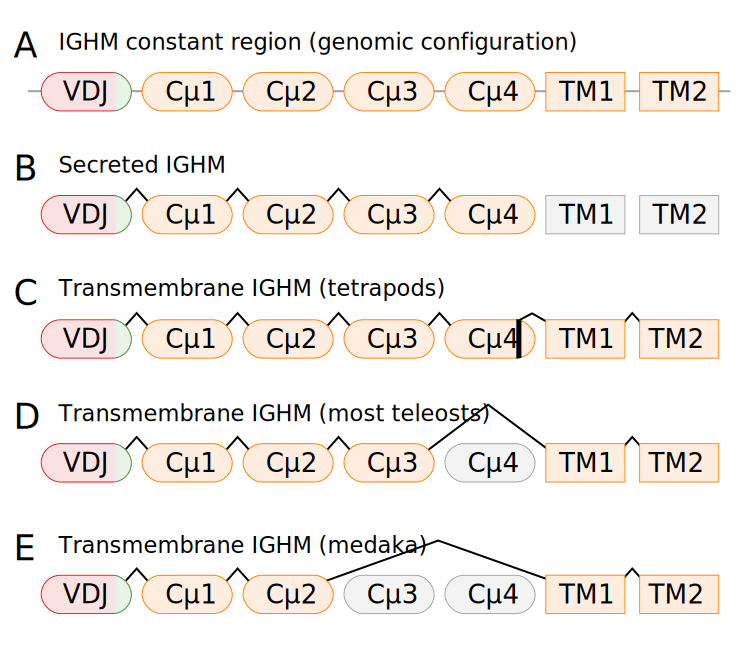
\includegraphics[width=0.8\textwidth]{output_files/figures/pdf/locus-teleost-igm-exons}
	\Caption{\igh{M} exon usage in bony vertebrates}{Schematic of \igh{M} splice patterns in different isoforms and taxonomic groups; (A) standard genomic (pre-splicing) configuration of \igh{M}, following VDJ recombination; (B) exon configuration of secreted \igh{M} (\igh{M-S}) in tetrapods and teleosts; (C) exon configuration of transmembrane \igh{M} (\igh{M-TM}) in tetrapods, demonstrating the use of a cryptic splice site in \cm{4}; (D) standard \igh{M-TM} exon configuration in teleosts, demonstrating the direct splicing of \cm{3} to TM1 and exclusion of \cm{4}; (E) unusual \igh{M-TM} exon configuration observed in medaka, in which both \cm{3} and \cm{4} are excluded. Adapted from Figure 3 of \parencite{fillatreau2013astonishing}.}
	\label{fig:teleost-igm-exons}
	\end{figure}
	
	\begin{figure}
	\centering
		\begin{subfigure}{0em}
        \phantomsubcaption{}
        \label{fig:nfu-locus-sashimi-a}
    \end{subfigure}
    \begin{subfigure}{0em}
        \phantomsubcaption{}
        \label{fig:nfu-locus-sashimi-b}
    \end{subfigure}
	\includegraphics[width=\textwidth]{output_files/figures/pdf/locus-nfu-sashimi}
	\Caption{Constant-region isoforms in \Nfu}{Coverage and Sashimi plots \parencite{katz2013sashimi} of \program{STAR}-aligned RNA-seq reads from \Nfu gut samples \parencite{smith2017microbiota}, demonstrating the splicing behaviour of \igh{1} constant-region isoforms and showing the read coverage of each exon and splice junction. (A) \igh{M} exon splicing, showing alternative splicing patterns of \igh{M-TM} and \igh{M-S}; (B) \igh{D} exon splicing, showing chimeric splicing of \cm{1} to \cd{1}.}
	\label{fig:nfu-locus-sashimi}
	\end{figure}
	
	\begin{figure}
	\centering
	\includegraphics[width = \textwidth]{output_files/figures/pdf/locus-nfu-ch-aln}
	\Caption{Cross-sublocus sequence similarity of constant-region exons in \Nfu \igh{}}{Heatmap of percentage sequence identity between amino-acid (left) and nucleotide (right) sequences of constant-region exons (excluding \igh{M-TM2} and \igh{D-TM2}) from the two subloci of \Nfu \igh{}, calculated using pairwise Needleman-Wunsch global alignments.}
	\label{fig:nfu-ch-aln}
	\end{figure}
	
	\begin{table}\centering
		\Caption{Cross-sublocus sequence similarity of constant-region exons in \Nfu}{Percentage sequence identities of pairwise Needleman-Wunsch global alignments between nucleotide (NT) or amino-acid (AA) sequences of corresponding exons from the two subloci of \Nfu \igh{}.}
	\input{output_files/tables/locus-nfu-ch-aln}
	\label{tab:nfu-ch-aln}
	\end{table}
	
\subsection{Variable regions}
\label{sec:nfu-locus-variable}
	
Variable-region gene segments in the turquoise-killifish \igh{} locus were identified with a variety of methods, depending on the type of gene segment being analysed (\Cref{sec:methods_comp_locus_segments}). \vh candidates were identified probabilistically using Hidden Markov Models constructed by \program{nhmmer} \parencite{wheeler2013nhmmer} from \program{PRANK} \parencite{loytynoja2014prank} multiple-sequence alignments of reference sequences, with the 3'-ends of each V-exon identified by the presence of a recombination-signal sequence (RSS) \parencite{schroeder2010immunoglobulins} and the 5'-ends refined using \program{IMGT-DomainGapAlign} \parencite{ehrenmann2011domaingapalign}. \jh candidates were also identified using \program{nhmmer}, with segment ends identified by the presence of an RSS (5') and a \sequence{GTA} splice-site motif (3') \parencite{magadan2011medaka}. Finally, \dh-segments, being too short and variable in sequence for HMM-based approaches to be effective, were identified by searching for pairs of flanking RSS sequences in opposite orientation, using fuzzy pattern-matching (with EMBOSS \program{FUZZNUC} \parencite{rice2000emboss}) to conserved RSS sequence motifs.
	 
In total, I identified 24 \vh-segments, 14 \dh-segments and 17 \jh-segments in the \Nfu locus (\Cref{tab:nfu-vh-coords,tab:nfu-dh-coords-seg,tab:nfu-jh-coords-seg}), of which the majority (17 \vh, 10 \dh and 8 \jh) were present in \igh{1}. Of the \vh segments identified, three contain premature stop codons, though none is out-of-frame; conversely, all the \dh and \jh segments identified appear to be in-frame and functional, with no premature stop codons. However, in all cases a minority of segments contain RSS sequences that deviate significantly from the expected consensus sequence (\Cref{tab:nfu-vh-coords,tab:nfu-dh-coords-rss5,tab:nfu-dh-coords-rss3,tab:nfu-jh-coords-rss}); it is unclear whether these sequences can recombine to successfully produce mature VDJ sequences \textit{in vivo}. In the case of the \vh segments, of the six sequences without clearly functional RSS sequences, three also contain premature stop codons, suggesting the changes to the RSS in these cases may arise from relaxed purifying selection on already-pseudogenised sequences.

Apart from these few exceptions, however, the recombination signal sequences (RSS) marking the ends of the \vh, \dh and \jh gene segments in the \Nfu locus otherwise strongly resemble those of other characterised teleosts, which in turn resemble those of non-teleost loci (\Cref{fig:nfu-rss-seqlogo-all,fig:nfu-rss-seqlogo-sep}). The overall heptamer and nonamer consensus sequences (\texttt{CACAGTG} for heptamers and \texttt{ACAAAAACC} for nonamers) closely matched those expected from the literature \parencite{schroeder2010immunoglobulins}, while in 88\,\% of cases the spacer region was within 1bp of the expected length (12bp for \dh-RSSs, 23bp for \vh- and \jh-RSSs); interestingly, the greatest number of \vh-RSSs had a 22bp (rather than 23bp) spacer, but this is unlikely to interfere with RSS functionality. Overall, the RSSs in the turquoise killifish appear to be supporting the normal operation of VDJ-recombination in this species.

Of the \vh, \dh and \jh segments identified, all but one of each type of segment is located within contiguous V-, D-, and J-regions within each sublocus, supporting a modified translocon configuration for turquoise-killifish \igh. The exceptions to this are \igh{1D01} and \igh{1J01}, which are embedded within the \igh{1} V-region, and a single \vh segment located in between the \igh{D} constant regions of the two subloci (\Cref{fig:nfu-locus-map-b}). The unusual location of \igh{1D01} and \igh{1J01} may represent the result of a transposition event within the \igh{} locus; however, their close colocalisation and 5' position within the \igh{1} sublocus, as well as the fact that neither has a close paralogue in \igh{2} (\Cref{fig:nfu-dj-alignment-b}), suggest that they may instead represent the remnant of a formerly present \igh{Z} constant region, as these typically have dedicated D/J segments independent of those serving \igh{M} (\Cref{sec:intro_teleost_loci}). Given its forward orientation, meanwhile, I assigned the orphaned \vh-segment to the \igh{1} sublocus as \igh{1V1-07}; however, if annotated correctly, it is unlikely to successfully recombine with segments in either sublocus due to its unusual location.
		
\begin{table}[hb]
	\centering
	\begin{threeparttable}
	\centering
	\caption{Number of functional \vh-segments and \vh-families in other teleost species}
	\label{tab:teleost-vh-counts}
	\begin{tabular}{ccccc}\toprule
	\multirow{2}{*}{	\textbf{Common Name}} & \multirow{2}{*}{\textbf{Species}} & \textbf{\# Functional} & \textbf{	\# \vh} & \multirow{2}{*}{\textbf{Source}} \\
	& & \textbf{\vh Segments} & \textbf{Families} & \\\midrule
	Zebrafish & \textit{Danio rerio} & 39 & 13\,\tnote{1} & \parencite{magadan2015fishrepertoires} \\
	Grass carp & \textit{Ctenopharyngodon idella} & 8 & 5\,\tnote{2} & \parencite{xiao2010grasscarp} \\
	Fugu & \textit{Takifugu rubripes} & 34 & 3 & \parencite{magadan2015fishrepertoires} \\
	Medaka & \textit{Oryzias latipes} & 35 & 6 & \parencite{fillatreau2013astonishing,magadan2011medaka} \\
	Stickleback & \textit{Gasterosteus aculeatus} & 49 & 4 & \parencite{magadan2015fishrepertoires} \\
	Turquoise killifish & \textit{Nothobranchius furzeri} & 21\,\tnote{3} & 6 & -- \\
	\bottomrule\end{tabular}
	\begin{tablenotes}
	\item[1] \vh families in zebrafish were identified based on 70\,\% (rather than 80\,\%) sequence identity.
	\item[2] It is not clear what clustering method or threshold was used to identify \vh families in grass carp.
	\item[3] Excluding \vh segments with nonsense or frameshift mutations, but not those with uncertain or missing RSS sequences.
	\end{tablenotes}
	\end{threeparttable}
\end{table}
	
\vh sequences within an \igh{} locus are conventionally grouped into families on the basis of nucleotide sequence identity, with a typical identity cutoff of 80\,\% \parencite{magadan2015fishrepertoires}. In order to group the \Nfu \vh genes into families, I performed pairwise Needleman-Wunsch global alignments on each pair of \vh sequences to obtain pairwise identity scores, followed by single-linkage clustering on the resulting identity matrix (\Cref{sec:methods_comp_locus_segments}). Cutting the dendrogram at 80\,\% sequence identity revealed a total of six \vh families, of which four contained more than one \vh segment (\Cref{fig:nfu-vh-families}); this number of \vh families in the \Nfu locus is roughly in line with those found in related species (\Cref{tab:teleost-vh-counts}). Of these, V1 and V2 make up the bulk (42\,\% and 29\,\% respectively) of the \vh segments in the locus. V2 and V4 are highly similar, and all the members of V4 are pseudogenised by premature stop codons; it may therefore be more appropriate to regard V4 as a pseudogenised subfamily of V2 than as a \vh family in its own right.

The total number of functional \vh segments in the turquoise-killifish locus is unusually small in comparison to the total numbers observed in many other teleost species (\Cref{tab:teleost-vh-counts}); however, the number of segments per sublocus is in line with the numbers seen in closely-related species (2 to 12 in medaka \parencite{magadan2011medaka}, 6 to 18 in stickleback \parencite{gambondeza2011stickleback,bao2010stickleback}), with the overall difference mainly arising from a difference in the number of subloci per locus. A similar pattern is observed with \jh segments, with similar numbers of segments per sublocus in turquoise killifish and closely-related species, especially medaka. It therefore appears that the per-sublocus segment diversity available to the turquoise killifish is similar to that of previously characterised species, with any difference in total available diversity at this level arising from differences in the number of functional subloci rather than the size of the V/D/J-regions \textit{per se}.

As can be seen from \Cref{fig:nfu-locus-synteny}, much of the V-, D- and especially J-region sequence in the \Nfu locus is syntenic between the two \igh{} subloci, with downstream portions of the \igh{2} V-region corresponding to downstream parts of the \igh{1} region. Of the seven \vh segments in \igh{2}, six have a corresponding segment on \igh{1} with which they share at least 97\,\% sequence identity (\Cref{fig:nfu-vh-families}), and these partner segments are largely (though not entirely) colinear in their ordering between the two subloci. A similar pattern can be observed for the D- and (especially) the J-regions: of the four \dh segments detectable in \igh{2}, three (\igh{2D02} to \igh{2D04}) are identical with another block of adjacent \dh segments in \igh{1} (\igh{1D05} to \igh{1D07}), while the \jh-regions exhibit almost complete sequence identity between the eight \jh segments of the main \jh region in \igh{1} and the eight \jh segments in \igh{2} (\Cref{fig:nfu-dj-alignment}).
		
Nevertheless, as is clear from \Cref{fig:nfu-locus-synteny}, there are large portions the \igh{1} variable region, including the first 25 kilobases of the V-region, for which no corresponding sequence exists in \igh{2}, and there are many \vh and \dh segments in \igh{1} (and a much smaller number in \igh{2}) for which no close homologue exists in the other sublocus. Taken together, these data are consistent with a model in which \igh{2} was produced via duplication and inversion of all or part of \igh{1}, followed by subsequent deletion events in the redundant, and structurally volatile, \igh{2} \vh and \dh regions. However, it is not clear at present how to distinguish between this model and an alternative one of expansion in \igh{1}, or how to explain why the \jh region is so much more conserved between subloci than either the \vh or \dh regions.

	
	\begin{figure}
	\centering
	\begin{subfigure}{0em}
	\phantomsubcaption{}
    \label{fig:nfu-vh-families-a}
    \end{subfigure}
    \begin{subfigure}{0em}
    \phantomsubcaption{}
    \label{fig:nfu-vh-families-b}
    \end{subfigure}
	\includegraphics[width=0.8\textwidth]{output_files/figures/pdf/locus-nfu-vh-families}
	\Caption{\vh families in the \Nfu \igh{} locus}{(A) Dendrogram of sequence similarity of \vh segments in the \Nfu \igh{} locus, arranged by single-linkage clustering on nucleotide sequence identity. The red line indicates the 80\,\% cutoff point for family assignment. (B) Heatmap of family relationships among \Nfu \vh segments, with shaded squares indicating families and red dots indicating pairwise nucleotide sequence identity of at least 80\,\%. In both subfigures, \vh families containing multiple segments are uniquely coloured, single-segment families are in grey, and segments from the \igh{2} sublocus are displayed in boldface.}
	\label{fig:nfu-vh-families}
	\end{figure}

\begin{figure}
\centering
	\centering
	\begin{subfigure}{0em}
	\phantomsubcaption{}
    \label{fig:nfu-dj-alignment-a}
    \end{subfigure}
    \begin{subfigure}{0em}
    \phantomsubcaption{}
    \label{fig:nfu-dj-alignment-b}
    \end{subfigure}
\includegraphics[width=0.6\textwidth]{output_files/figures/pdf/locus-nfu-dj-aln}
\Caption{Cross-sublocus sequence similarity of \dh and \jh gene segments in \Nfu \igh{}}{Heatmap of percentage nucleotide sequence identities of Needleman-Wunsch global alignments between (A) \dh and (B) \jh gene segments in \igh{1} vs \igh{2}, revealing syntenic runs of highly similar sequences across both subloci.}
\label{fig:nfu-dj-alignment}
\end{figure}	
	
	\begin{figure}
	\centering
	\includegraphics[width=\textwidth]{output_files/figures/pdf/locus-nfu-rss-seqlogo-all}
	\Caption{Recombination signal sequences in \Nfu \igh{}}{(A) Sequence composition of conserved heptamer sequences across all \Nfu heavy-chain RSSs; (B) length distribution of unconserved spacer sequences in \Nfu heavy-chain RSSs; (C) sequence composition of conserved heptamer sequences across all \Nfu heavy-chain RSSs.}
	\label{fig:nfu-rss-seqlogo-all}
	\end{figure}
	
\FloatBarrier
\clearpage

\section{The \igh{} locus in \xma}
\label{sec:xma-locus}
	
	The turquoise-killifish \igh{} locus shares many features with other characterised teleost loci, including a modified tandem-translocon configuration with intact \vh, \dh, \jh and constant regions (\Cref{fig:nfu-locus-map-b}), a four-exon secreted configuration of \igh{M} (\Cref{fig:nfu-locus-sashimi-a}), an expanded \igh{D} constant region with tandem \cd{}-exon block repeats (\Cref{fig:nfu-locus-sashimi-b,fig:nfu-locus-map-b},), a conserved RSS structure (\Cref{fig:nfu-rss-seqlogo-all}), and a chimeric \cm{1} in \igh{D} (\Cref{fig:nfu-locus-sashimi-b}). However, it also exhibits many ideosyncratic features that differ from those observed in most characterised teleost loci, including an unusually small number of \vh segments (\Cref{fig:nfu-vh-families} and \Cref{tab:teleost-vh-counts}), a four-exon \cm{1}-\cm{2}-TM1-TM2 configuration of transmembrane \igh{M} (\Cref{fig:nfu-locus-sashimi-a}), an inverted sublocus present in antisense (\Cref{fig:nfu-locus-map-b}), and a complete absence of \igh{Z}.
	
Many of these peculiarities, including the unusual \igh{M-TM} splicing pattern, inverted sublocus, and lack of \igh{Z}, are shared with the \igh{} locus of medaka (\textit{Oryzias latipes}), which is the closest relative of \textit{Nothobranchius furzeri} to have its immunoglobulin heavy chain locus characterised prior to this study \parencite{magadan2011medaka}. Given the close relationship between the two species, the shared unusual features of their \igh{} loci suggested a common origin of these traits  in the common ancestor of both species. If this hypothesis were correct, one would expect \igh{Z} to also be absent in any other descendents of this common ancestor, including other cyprinodontiform species.

To investigate this hypothesis further, I performed a complete characterisation of the \igh{} locus in the platyfish \textit{Xiphophorus maculatus}, another cyprinodontiform species that has seen widespread use as a model organism \parencite{schartl2013platyfish}. Surprisingly, the \Xma locus possessed none of the unusual features shared between the turquoise-killifish and medaka loci, strongly suggesting independent loss of \igh{Z} in \Nfu and medaka and implying a high level of volatility in \igh{} locus structure in this group of teleost fishes.

\subsection{Overall structure}
\label{sec:xma-locus-structure}
	
As was the case with the \Nfu \igh{} locus, I identified candidate genome scaffolds from the most recent \xma genome assembly (Genbank accession GCA\_002775205.2) by aligning them to \igh{} gene segments from zebrafish, stickleback and medaka, supplemented in this case with segments from the newly-characterised \Nfu locus itself. In contrast to the more fragmented results in \Nfu, this process identified a single sequence region on one chromosome of the \Xma locus, which I extracted and characterised as described for the assembled \Nfu locus (\Cref{sec:nfu-locus}) without the need for further sequencing or assembly.

The \Xma \igh{} locus so identified occupies roughly \kb{293} on chromosome 16 (scaffold NC\_036458.1; \Cref{fig:xma-locus-map-a}). Unlike in turquoise killifish and medaka, all identified gene segments share a common orientation; no evidence of a second sublocus in antisense could be identified. In stark contrast with both turquoise killifish and medaka, the single ``sublocus'' comprising \Xma \igh{} contains not one but two \igh{Z} constant regions, along with a hugely extended V-region extending over almost \kb{250} and containing more than 120 \vh-segments (\Cref{fig:xma-locus-map-b}). This enormous \vh-diversity exceeds that of almost all previously-characterised teleost \igh{} loci (\Cref{sec:intro_teleost_loci}), while the presence of multiple \igh{Z} constant regions without intervening \igh{M} or \igh{D} is also highly unusual \parencite{fillatreau2013astonishing}. 

Even cursory examination of the \Xma \igh{} locus is therefore sufficient to reveal a unique and highly interesting structure with many unexpected differences from both turquoise killifish and medaka (\Cref{fig:species-tree-small}, columns 1-5). In particular, since \Xma is more closely related to \Nfu than either is to medaka, the presence of \igh{Z} in the former strongly suggests at least two independent loss events in the lineage containing turquoise killifish and medaka, indicating an unexpected level of volatility in the evolution of this important isotype.
 
	\begin{figure}
	\centering
	\includegraphics[width=\textwidth]{output_files/figures/pdf/locus-xma-map}
	\Caption{The immunoglobulin heavy chain (\igh{}) locus in \xma}{(A) Position of the \igh{} locus on chromosome (group) 16 of the \Xma genome. (B) Arrangement of \vh, \dh, \jh and constant-region gene segments on the \Xma \igh{} locus. (C) Detailed map of the \igh{Z1}, \igh{Z2} and \igh{M/D} constant regions, indicating the position and identity of the constant-region exons and the exon composition of expressed \igh{} isoforms in \Xma. Note change of orientation between subfigures (A) and (B-C).}
	\begin{subfigure}{0em}
        \phantomsubcaption{}
        \label{fig:xma-locus-map-a}
    \end{subfigure}
    \begin{subfigure}{0em}
        \phantomsubcaption{}
        \label{fig:xma-locus-map-b}
    \end{subfigure}
    \begin{subfigure}{0em}
        \phantomsubcaption{}
        \label{fig:xma-locus-map-c}
    \end{subfigure}
	\label{fig:xma-locus-map}
\end{figure}

\begin{figure}
\centering
\includegraphics[width=\textwidth]{output_files/figures/pdf/locus-species-phenotypes}
\vspace{0.5em}
\Caption{Important \igh{} phenotypes in turquoise killifish, southern platyfish, and medaka}{Cladogram of the evolutionary relationship between southern platyfish (\xma), turquoise killifish (\nfu) and medaka (\species{Oryzias}{latipes}), with three-spined stickleback (\species{Gasterosteus}{aculeatus}) as an outgroup. The state of various \igh{} phenotypes of interest are annotated to the right of the tree; states deviating from the expected teleost configuration are in bold.}
\label{fig:species-tree-small}
\end{figure}
	
\subsection{Constant regions}
\label{sec:xma-locus-constant}
	
As discussed briefly in \Cref{sec:xma-locus-structure}, the \Xma \igh{} locus contains two distinct \igh{Z} constant regions: one in the usual position immediately preceding the \igh{M}-associated D- and J-regions, the other, unexpectedly, at the far 5'-extremity of the locus (\Cref{fig:xma-locus-map-b}). Both \igh{Z} constant regions occupy the expected configuration, with four \cz{} exons, two transmembrane exons, and a secretory tail (\Cref{fig:xma-locus-map-c}, \Cref{tab:xma-ch-coords}). However, in contrast to the duplicate constant regions in \Nfu, the two \igh{Z} constant regions in \Xma are quite distinct from each other in sequence, with an average of only \pc{64} nucleotide and \pc{48} amino-acid sequence identity between corresponding \cz{} exons (\Cref{fig:xma-cz-aln}, \Cref{tab:xma-cz-aln}). This unexpectedly high level of sequence divergence suggests a relatively ancient duplication event, and raises the possibility that the lineage giving rise to \Nfu may have lost not one, but two distinct \igh{Z} constant regions.
	
\begin{table}
	\centering
	\Caption{Sequence similarity between \igh{Z} constant-regions in \Xma}{Percentage sequence identities of pairwise Needleman-Wunsch global alignments between nucleotide (NT) or amino-acid (AA) sequences of corresponding \cz{} exons from the two \igh{Z} constant regions of \Xma \igh{}.}
	\input{output_files/tables/locus-xma-cz-aln}
	\label{tab:xma-cz-aln}
\end{table}

While the state of \igh{Z} constant regions differs markedly between \Xma and \Nfu, the configurations of the \igh{M} and \igh{D} constant regions of the two species are quite similar, with a {\cm{1}-\cm{2}-\cm{3}-\cm{4}-TM1-TM2} configuration for \igh{M} and a {\cd{1}-(\cd{2}-\cd{3}-\cd{4})$_2$-\cd{5}-\cd{6}-\cd{7}-TM1-TM2} configuration for \igh{D} (\Cref{fig:xma-locus-map-b,fig:xma-locus-map-c}, \Cref{tab:xma-ch-coords}). In the \Xma locus, these constant regions and \igh{Z2} adopt the standard configuration seen in comparatively simple teleost \igh{} loci like those of zebrafish and fugu, with a {\vh-\dh-\jh-\textbf{CZ}-\dh-\jh-\textbf{CM}-\textbf{CD}} arrangement that allows the choice between \igh{Z} and \igh{M/D} usage to be made via the choice of \dh segment during VDJ-recombination. However, whether such a mechanism is also responsible for the choice between these constant regions and \igh{Z1}, which lies more than \kb{200} away and upstream of the great majority of \vh segments in the locus (\Cref{sec:xma-locus-variable}) is questionable.

In order to investigate the expressed isoforms present in \Xma, I aligned published RNA-sequencing reads from various platyfish tissues (BioProject accession PRJNA420092, all libraries, \Cref{tab:rnaseq-sources}) to the \igh{Z} and \igh{M/D} constant regions with \program{STAR}. The results indicate the expected six-exon transmembrane configuration in both \igh{Z1} and \igh{Z2}, as well as a secretory form of \igh{Z1} comprising \cz{1} to \cz{4} plus a \bp{23} secretory tail formed by a transcriptional run-on event from \cz{4} (\Cref{fig:xma-locus-sashimi-z1,fig:xma-locus-sashimi-z2}). However, while an in-frame secretory tail of similar length (\bp{20}) can be found in \igh{Z2}, it does not appear to be expressed in the read sets analysed here, suggesting that \igh{Z2} may only be expressed in transmembrane form in the individuals sampled (\Cref{fig:xma-locus-sashimi-z2}).

Meanwhile, the results for \igh{D} (\Cref{fig:xma-locus-sashimi-d}) indicate a similar configuration to that observed in turquoise killifish, with a chimeric \cm{1} followed by 10 \cd{} exons and two transmembrane exons; as in \Nfu, neither a dedicated \igh{D} secretory exon nor a post-\cd{7} secretory tail was identified, suggesting that \igh{D} may be produced solely in transmembrane form in \Xma. Secretory \igh{M} (\igh{M-S}) was also found to occupy the same four-exon configuration seen in turquoise killifish and elsewhere. However, the configuration observed for transmembrane \igh{M} (\igh{M-TM}) did not correspond to the four-exon structure shared between turquoise killifish and medaka (\Cref{fig:xma-locus-sashimi-m,fig:nfu-locus-sashimi-a}); rather, \igh{M-TM} in \Xma occupies the five-exon configuration seen in most characterised teleosts (\Cref{fig:teleost-igm-exons-d}). This surprising difference indicates that two different splice configurations of \igh{M-TM} persist in the cyprinodontiform lineage, and raises the question of what, if any, functional difference arises from the presence or absence of \cm{3} in transmembrane \igh{M} in different species. However, it remains unclear whether this pattern of exon usage (\Cref{fig:species-tree-small}) is the result of independent changes in medaka and turquoise killifish or of a reversion in \Xma to the primitive teleost configuration.
	
\begin{figure}
	\includegraphics[width=\textwidth]{output_files/figures/pdf/locus-xma-sashimi}
	    \begin{subfigure}{0em}
        \phantomsubcaption{}
        \label{fig:xma-locus-sashimi-z1}
    \end{subfigure}
    \begin{subfigure}{0em}
        \phantomsubcaption{}
        \label{fig:xma-locus-sashimi-z2}
    \end{subfigure}
	\begin{subfigure}{0em}
        \phantomsubcaption{}
        \label{fig:xma-locus-sashimi-m}
    \end{subfigure}
    \begin{subfigure}{0em}
        \phantomsubcaption{}
        \label{fig:xma-locus-sashimi-d}
    \end{subfigure}
	\Caption{Constant-region isoforms in \Xma}{Coverage and Sashimi plots \parencite{katz2013sashimi} of STAR-aligned RNA-seq reads from \Xma samples, demonstrating the splicing behaviour of \igh{} constant-region isoforms and showing the read coverage of each exon and splice junction. (A) \igh{Z1} exon splicing, showing alternative use of the \cz{4}/TM1 splice junction and the post-\cz{4} secretory tail; (B) \igh{Z2} exon splicing, showing the apparent lack of expression of the \igh{Z2} secretory isoform; (C) \igh{M} exon splicing, showing alternative splicing patterns of \igh{M-TM} and \igh{M-S}; (D) \igh{D} exon splicing, showing chimeric splicing of \cm{1} to \cd{1}.}
	\label{fig:xma-locus-sashimi}
	\end{figure}

	
\subsection{Variable regions}
\label{sec:xma-locus-variable}

In total, I identified 125 \vh segments, 14 \dh segments and 15 \jh segments in the \Xma \igh{} locus (\Cref{fig:xma-locus-map-b}). Of these, exactly one \vh (\igh{V01-01}), \dh (\igh{DZ01}) and \jh (\igh{JZ01}) lie upstream of the \igh{Z1} constant region, indicating that the variable-region sequence diversity available to this isotype is limited to a single VDJ combination. In contrast, the variable region between the end of \igh{Z1} and the start of \igh{Z2} is highly expanded, with 124 tightly-clustered \vh segments -- more than five times the total number seen in \Nfu, and more than seven times the number in the largest \Nfu sublocus. Of these 124 \vh segments, 106 (\pc{86}) are apparently functional, with the remainder pseudogenised by a variety of frameshift mutations, nonsense mutations, or truncation events (\Cref{tab:xma-vh-coords-1,tab:xma-vh-coords-2,tab:xma-vh-coords-3,tab:xma-vh-coords-4,tab:xma-vh-coords-5}); it remains to be seen whether \igh{V01-01} is also capable of recombining with \dh segments downstream of the \igh{Z1} constant region, and so constitutes part of the range of VDJ combinations available to the other constant regions. The \vh sequences in the \Xma locus are much more tightly packed than in the \Nfu locus, consistent with a lower overall prevalence of repetitive regions (21\,\%) in the \Xma genome \parencite{yuan2018repeats}.
	
In total, the \vh regions in \Xma \igh{} fall into 23 families, of which eight contain multiple segments (\Cref{fig:xma-vh-families-tree,fig:xma-vh-families-map}); strikingly, the single \vh segment serving \igh{Z} (\igh{V01-01}) represents a separate family which is distinct from any other segment in the locus. To further investigate the evolutionary history of these families, I aligned the \vh segments from both the \Xma and \Nfu \igh{} loci together with \program{PRANK}, and used the resulting alignment to construct a phylogenetic tree with \program{RAxML} \parencite{stamatakis2014raxml8,stamatakis2005raxml3,stamatakis2006raxml6}; the resulting tree (\Cref{fig:nfu-xma-vh-tree-nt}) revealed a clear interrelationship between the largest families in both loci (\Xma V02 and \Nfu V1), with a similar relationship observed for the second-largest families (\Xma V03 and \Nfu V2). 
In accordance with the close sequence relationship noted in \Cref{sec:nfu-locus-variable}, \Nfu V4 falls comfortably within the V03/V2 subtree, supporting its status as a pseudogenised subfamily of \Nfu V2.
		
In addition to its highly expanded \vh region, the variable region of the \Xma locus is unusual in the arrangement of its \dh and \jh segments (\Cref{tab:xma-dh-coords-seg,tab:xma-jh-coords-seg}): in addition to the relatively densely-packed blocks of four \dh and eight \jh segments between \igh{Z2} and \igh{M}, and the smaller groups of three \dh segments and one \jh segment between the last \vh segment and \igh{Z2}, small numbers of \dh and \jh segments are interspersed between blocks of \vh segments in the extended V-region between \igh{Z1} and \igh{Z2} (\Cref{fig:xma-locus-map-b}). Many of these segments are arranged such that groups of one or two \dh segments are closely associated with a single \jh segment, raising the possibility of a more cluster-like behaviour in which each VDJ block acts as a distinct recombination unit. However, the presence of larger D- and J-regions more closely upstream of the constant regions suggests a more conventional translocon behaviour; it remains to be seen which of these traditional models of antigen-receptor structure more closely matches the \textit{in vivo} recombination behaviour of this locus.
		
Finally, as is the case with \Nfu, the recombination signal sequences (RSSs) in \Xma \igh{} correspond closely to the standard expectations across the vertebrates, with the expected heptamer and nonamer consensus sequences and spacer length distributions (\Cref{fig:xma-rss-seqlogo-all,fig:xma-rss-seqlogo-sep}, 97.6\,\% of RSS spacers within \bp{1} of the expected conserved length).	

	\begin{figure}
		\begin{subfigure}{0em}
        \phantomsubcaption{}
        \label{fig:xma-rss-seqlogo-all-heptamer}
    \end{subfigure}
    \begin{subfigure}{0em}
        \phantomsubcaption{}
        \label{fig:xma-rss-seqlogo-all-spacer}
    \end{subfigure}
    \begin{subfigure}{0em}
        \phantomsubcaption{}
        \label{fig:xma-rss-seqlogo-all-nonamer}
    \end{subfigure}
	\includegraphics[width=\textwidth]{output_files/figures/pdf/locus-xma-rss-seqlogo-all}
	\Caption{Recombination signal sequences in the \Xma \igh{} locus}{(A) Sequence composition of conserved heptamer sequences across all \Xma heavy-chain RSSs; (B) length distribution of unconserved spacer sequences in \Xma heavy-chain RSSs; (C) sequence composition of conserved heptamer sequences across all \Xma heavy-chain RSSs.}
	\label{fig:xma-rss-seqlogo-all}
	\vspace{1em}
	\end{figure}
	
	\begin{figure}
	\centering
	\includegraphics[width=\textwidth]{output_files/figures/pdf/locus-xma-vh-families-tree}
	\Caption{Dendrogram of \vh families in the \Xma \igh{} locus}{Dendrogram of sequence similarity of \vh segments in the \Xma locus, arranged by single-linkage clustering on nucleotide sequence identity. The red line indicates the 80\,\% cutoff point for family assignment, while branch colour indicates family membership:  \vh families containing multiple segments are uniquely coloured, while single-segment families are in grey.}
	\label{fig:xma-vh-families-tree}
	\end{figure}
	
	\begin{figure}
	\centering
	\includegraphics[width=0.8\textwidth]{output_files/figures/pdf/locus-comp-vh-tree}
	\Caption{Evolutionary relationships between \vh families in \Xma and \Nfu}{Phylogenetic tree of evolutionary relationships between \igh{} \vh segments in \Nfu and \Xma, as inferred from the nucleotide sequences of \vh segments from both loci. Note the close interrelationship between the largest \vh families in each species (red zone), and similarly between the second-largest families in each species (blue zone). The red diamond indicates the location of the outgroup, which is composed of zebrafish \textit{TRB} V-segments.}
	\label{fig:nfu-xma-vh-tree-nt}
	\end{figure}
		
\FloatBarrier

\clearpage

\section{\igh{} constant-region evolution in the Cyprinodontiformes}
\label{sec:locus_comparative}

The characterised \igh{} loci of \nfu and \xma together reveal a high degree of variability in structure and function across the Atherinomorpha, the parent clade of the Cyprinidontiformes (including \Nfu and \Xma) and medaka (\Cref{fig:species-tree-large-taxa}). Several unusual features (including the loss of \igh{Z}, an inverted sublocus, and an unusual splicing pattern of \igh{M-TM}) are shared between medaka and turquoise killifish, but absent in \Xma (\Cref{fig:species-tree-small}), indicating either an independent origin in the former two species or a reversion to the primitive state in the latter. In addition, the copy number, exon usage and orientation of constant regions of other isotypes differs among the three species, raising the further question of how, when and why these changes occurred. 

In order to investigate a subset of these questions with a greater degree of phylogenetic resolution, I identified and analysed \igh{} constant regions in the genomes of ten additional cyprinodontiform species (\Cref{fig:species-tree-large-taxa}, \Cref{tab:cyprinodontiform-genomes}), as well as in a new and improved genome assembly of medaka (Genbank accession GCA\_002234675.1), using the same methods described for \Nfu and \Xma (\Cref{sec:nfu-locus-constant,sec:nfu-locus-variable}). I then grouped the constant-region exons so identified (\Cref{fig:ch-tree-all}) by order, exon type and spatial proximity to identify contiguous constant-regions, enabling the presence/absence and number of constant regions of each isotype to be estimated for each species. The results of this analysis (\Cref{fig:multispecies-ch-regions}, \Cref{tab:multispecies-ch-regions-1,tab:multispecies-ch-regions-2,tab:multispecies-ch-regions-3}) demonstrate that every species investigated possesses at least one complete \igh{M} and \igh{D} constant region in tandem, with several species exhibiting multiple such regions. Apart from \Nfu and medaka, only \textit{Nothobranchius orthonotus} was identified as clearly possessing adjacent constant regions in opposite orientation, indicating the presence of at least one sublocus in antisense; however, the fragmented nature of the \igh{} locus assembly in many analysed species prevented a confident exclusion of such configurations in other cases.

\begin{table}[bh!]
\centering
\begin{threeparttable}
\begin{tabular}{>{\itshape}l>{\itshape}llc}\toprule
\textnormal{\textbf{Genus}} & \textnormal{\textbf{Species}} & \textbf{Common Name} & \textbf{GenBank Assembly Accession}\\\midrule
Nothobranchius & furzeri & Turquoise killifish & NA\tnote{1}\\\midrule
Xiphophorus & maculatus & Southern platyfish & GCA\_002775205.2\\
Austrofundulus & limnaeus & -- & GCA\_001266775.1\\
Fundulus & heteroclitus & Mummichog & GCA\_000826765.1\\
Poecilia & formosa & Amazon molly & GCA\_000485575.1\\
Poecilia & reticulata & Guppy & GCA\_000633615.1\\
Cyprinodon & variegatus & Sheepshead minnow & GCA\_000732505.1\\
Kryptolebias & marmoratus & Mangrove rivulus & GCA\_001649575.1\\\midrule
Aphyosemion & australe & Lyretail panchax & NA\tnote{2}\\
Callopanchax & toddi & -- & NA\tnote{2}\\
Pachypanchax & playfairii & Golden panchax & NA\tnote{2}\\
Nothobranchius & orthonotus & Spotted killifish & NA\tnote{2}\\\midrule
Oryzias & latipes & Medaka & GCA\_002234675.1\\
\bottomrule\end{tabular}
\begin{tablenotes}
\item[1] Willemsen \textit{et al.} \parencite{willemsen2019popgen}
\item[2] Cui \textit{et al.} \parencite{cui2019annual}
\end{tablenotes}
\end{threeparttable}
\vspace{0.5em}
\caption{Genome assemblies used to identify \igh{} locus sequences in cyprinodontiform fishes}
\label{tab:cyprinodontiform-genomes}
\end{table}

\begin{figure}
\centering
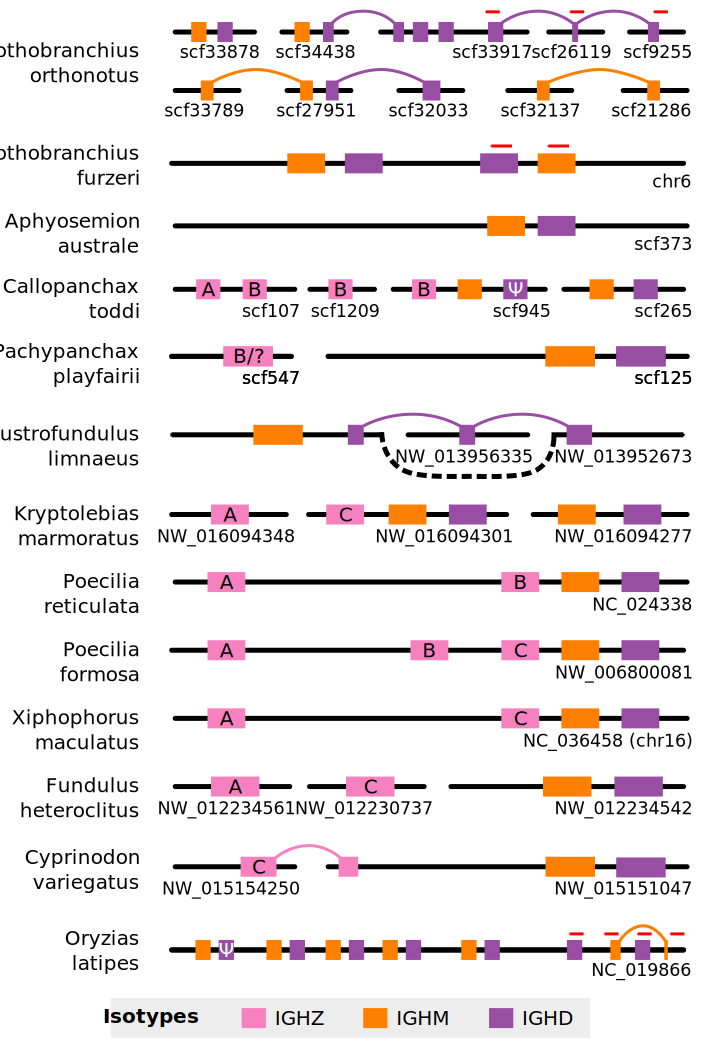
\includegraphics[width=0.9\textwidth]{output_files/figures/pdf/locus-multispecies-ch-regions}
\Caption{Constant-region organisation in the Atherinomorpha}{Schematic of \igh{} constant regions in the genomes of thirteen species from the Atherinomorpha. Scaffold orientation is given by the black arrows; constant regions are oriented left-to-right unless otherwise specified (red arrows). Links between regions on different scaffolds indicate that exons from what appears to be the same constant region are distributed across multiple scaffolds in the order indicated; the order of unlinked scaffolds is arbitrary. The isotype of each region is given by its colour; \igh{Z} regions are further annotated with their subclass (\Cref{fig:species-tree-large-ighz}). Clearly pseudogenised constant regions are indicated by $\Psi$. Isotype length, scaffold length, and scaffold position are not to scale. Variable regions and lone, isolated constant-region exons are not shown.}
\label{fig:multispecies-ch-regions}
\end{figure}

In addition to at least one \igh{M} and \igh{D} constant region, the majority of species analysed (8 out of 13) were also found to possess at least one complete \igh{Z} constant region; of the exceptions, \species{A.}{limnaeus} exhibits an orphaned, pseudogenised \igh{Z-TM1} exon but no \cz{} exons in the current genome assembly (\Cref{fig:multispecies-ch-regions}, \Cref{tab:multispecies-ch-regions-2}), while \species{O.}{latipes}, \species{A.}{australe}, \Nfu and \species{N.}{orthonotus} possess no \igh{Z} exons at all. Annotating the tree from \Cref{fig:species-tree-large-taxa} with the \igh{Z} status of each species (\Cref{fig:species-tree-large-ighz}) confirms that the loss of \igh{Z} in turquoise killifish (and related species) and medaka represent two distinct deletion events, with \textit{Austrofundulus limnaeus} potentially representing a second independent loss of \igh{Z} within the Cyprinodontiformes and a third within the Atherinomorpha.

\begin{figure}
\centering
\includegraphics[width=0.9\textwidth]{output_files/figures/pdf/locus-species-cladogram-ighz}
\Caption{\igh{Z} has been lost multiple times independently in the Atherinomorpha}{Cladogram of species reproduced from \Cref{fig:species-tree-large-taxa}, annotated according to the known (tip nodes) or inferred (internal nodes) presence or absence of intact \igh{Z} constant regions in each species. Large coloured points on the cladogram denote sites of hypothesised state changes; \igh{Z} is assumed to be primitively present in the clade and losses to be irreversible. The currently-available genome assembly of \textit{A. limnaeus} (dark pink) contains one pseudogenised \igh{Z-TM1} exon and no \cz{} exons.}
\label{fig:species-tree-large-ighz}
\end{figure}

Apart from its repeated loss within the lineage, a second striking feature of \igh{Z} within the Cyprinodontiformes is its frequent presence in multiple copies per \igh{} locus, with a geometric mean of 1.929 regions per \igh{Z}-bearing locus. On average (geometric mean), the species analysed have approximately 1.62 \igh{Z} constant regions per \igh{M} constant region, and the same ratio vs \igh{D}, suggesting a more complex evolutionary history than can be captured by a simple presence/absence metric. Concordantly, phylogenetic analysis (\Cref{fig:multispecies-cz-tree}, tree built using \program{PRANK} and \program{RAxML} on concatenated \cz{1}--\cz{4} exon sequences) reveals three distinct lineages (or subclasses) of \igh{Z} constant regions in the Cyprinidontiformes, \igh{ZA} to \textit{C}, each of which is present in multiple different species and appears to have been present in the common ancestor of the eight \igh{Z}-bearing species analysed (\Cref{fig:multispecies-cz-subclasses}).

\begin{figure}
	\centering
	\includegraphics[width=0.9\textwidth]{output_files/figures/pdf/locus-comp-cz-tree}
	\Caption{\igh{Z} constant regions in the Cyprinodontiformes constitute three distinct subclasses}{Phylogram of concatenated \cz{1}--\cz{4} nucleotide sequences from \igh{Z}-bearing species in \Cref{tab:cyprinodontiform-genomes}, with \cm{1}--\cm{4} sequences from two species as an outgroup (in orange). Nodes with bootstrap support of less than 65\,\% are collapsed into polytomies. Major clades (A--C) are annotated on the right. Support values indicate the result of rapid bootstrapping by \program{RAxML} across 1000 replicates.}
	\label{fig:multispecies-cz-tree}
\end{figure}

\begin{figure}
\centering
\includegraphics[width=0.8\textwidth]{output_files/figures/pdf/locus-species-cladogram-cz-subclasses}
\begin{minipage}{0.7\textwidth}
\footnotesize
\begin{threeparttable}
\begin{tablenotes}
\item[1] \textit{P. playfairii} \igh{Z} \cz{1}--\cz{2} appear to be derived from \igh{Z-B}, while the other exons are of uncertain subclass origin (\Cref{fig:ppl-cz-aln}).
\end{tablenotes}
\end{threeparttable}
\end{minipage}
\Caption{Distribution of \igh{Z} subclasses in the Atherinomorpha}{Cladogram of atherinomorph species with characterised \igh{} constant regions, annotated with the number of regions belonging to each \igh{Z} isotype in each species. All three subclasses are present in at least one species in both major branches of the cyprinodontiform clade, suggesting that they were all present in the common ancestor of this grouping.}
\label{fig:multispecies-cz-subclasses}
\end{figure}


Only one \igh{Z} constant region from the analysed species could not be confidently assigned to one of these three subclasses, namely the single \igh{Z} of \species{Pachypanchax}{playfairii} (\Cref{fig:multispecies-cz-tree}). In order to more closely investigate the relationships of \igh{Z} in this species, I aligned the exon sequences of \species{P.}{playfairii} \cz{1}--\cz{4} separately to the \cz{} exons of all other \igh{Z}-bearing species and plotted the distribution of alignment scores in each case (\Cref{fig:ppl-cz-aln}). The results show a striking difference in alignment behaviour between the exons, with \cz{1} and \cz{2} aligning significantly more strongly to exons from the B subclass and \cz{3} and \cz{4} showing more ambiguous affinity for either A- or C-subclass sequences. This unexpected behaviour indicates that the \species{P.}{playfairii} \igh{Z} sequence is the result of a deletion or fusion event combining the first two exons of a B-subclass \igh{Z} constant region with the latter exons of a constant region from another subclass, resulting in a chimeric gene with ambiguous ancestry.

\begin{figure}
	\centering
	\includegraphics[width=0.8\textwidth]{output_files/figures/pdf/locus-ppl-cz-aln}
	\Caption{Subclass affinity of \igh{Z} in \species{Pachypanchax}{playfairii}}{Boxplots of Needleman-Wunsch alignment scores between the amino-acid sequences of \species{P.}{playfairii} \cz{} exons and those of seven other \igh{Z}-bearing cyprinodontiform species, demonstrating the differing affinity of different \species{P.}{playfairii} exons for each of the three \igh{Z} subclasses. Pairwise $p$-values were computed using nonparametric Mann-Whitney $U$ tests ($*: 0.01 < p \leq 0.05;~**: 0.001 < p \leq 0.01;~***: p \leq 0.001$).}
	\label{fig:ppl-cz-aln}
\end{figure}
	
In summary, in addition to the still-universal primitive antibody classes \igh{M} and \igh{D}, the cyprinodontiforms ancestrally possessed at least three variants of \igh{Z}, giving rise to multiple subclasses of \igh{Z} constant regions evolving in parallel across the clade. Each of these subclasses appears to have been lost in multiple cyprinodontiform species, with different species showing distinct patterns of retention and loss, and in at least one lineage -- that of \species{Pachypanchax}{playfairii} -- two different \igh{Z} lineages have fused to produce a chimeric isotype. All three subclasses are missing from a subset of species in the Nothobranchiidae (including \nfu), and also appear to have been independently lost in \species{Austrofundulus}{limnaeus}. Taken together, these data suggest a high degree of complexity and volatility in the evolution of mucosal adaptive immunity in the Cyprinodontiformes.

\newpage

\section{Discussion}

The teleost fishes are the largest and most diverse group of vertebrates, with nearly 30,000 species comprising almost half of extant vertebrate diversity \parencite{ravi2018divergent}. Of this vast variety of teleosts, only a few species, mostly those used extensively in aquaculture or scientific research, have undergone extensive study with regard to their immunoglobulin gene loci (\Cref{sec:intro_teleost_loci}). Studies in these model species have revealed a high level of structural diversity among teleost \igh{} loci, with huge variation in both size and organisation, as well as the existence of three distinct antibody isotypes in fish, of which two (\igh{M} and \igh{D}) are shared with tetrapods and one (\igh{Z}) appears to be teleost-specific. However, in many large and important teleost lineages, the genetic basis of B-cell-mediated humoral immunity remains unknown.

In this chapter, I presented two complete and ten partial assemblies of \igh{} loci from the Cyprinodontiformes, a diverse clade of primarily freshwater fishes for which no such loci have previously been characterised. The two complete assemblies were of the \igh{} loci of the turquoise killifish \nfu and the southern platyfish \xma, two important model species with an estimated divergence time of less than 80 Mya \parencite{hughes2018teleostphylo}. Despite their close relationship, these species show radically different locus organisations, with huge differences in VDJ number (24 \vh segments in \Nfu versus 125 in \Xma), locus organisation (two small subloci in opposite sense in \Nfu, one large unitary locus in \Xma) and isotype availability (no \igh{Z} in \Nfu, two distinct \igh{Z} regions in \Xma), as well as more subtle but still-important distinctions like differences in constant-region splicing behaviour (four exons in \Nfu \igh{M-TM}, five in \Xma). These results are consistent with previous findings of highly-diverse teleost loci and support a process of rapid evolution in the \igh{} locus. Characterisation of the constant regions of a further ten cyprinodontiform species confirmed this finding, with several groups of closely-related species (e.g. \nfu, \species{Nothobranchius}{orthonotus} and \species{Callopanchax}{toddi}) showing highly divergent locus structures and constant-region availability.

It is interesting to speculate on the origins of this extremely rapid diversification in gene structure. Very little is known about the relationship between environmental context and immune locus structure; it is possible that part of the variety in \igh{} gene locus structure in the Cyprinodontiformes represents divergent adaptations to different immune environments. Alternatively, this diversification may be primarily the result of unusually high rates of stochastic, non-adaptive changes in gene structure in germline \igh{}. Finally, at least some of the difference between locus structures in different species is likely to be attributable to differences in assembly quality; for example, the characterisation of medaka constant regions presented here contains many fewer unusual or incomplete constant regions than that presented in the published medaka \igh{} locus \parencite{magadan2011medaka}, primarily due to the increased quality of the more recent medaka genome assemblies.

Before the publication of this work, only two teleost species (medaka and channel catfish) were known or thought to lack the \igh{Z} antibody isotype from their \igh{} loci, out of more than ten species with published locus characterisations. This relative rarity of observed absence, combined with the apparent importance of \igh{Z} in teleost mucosal immunity, suggested that the loss of \igh{Z} was likely to be a rare and unusual event. However, in addition to confirming the absence of \igh{Z} in medaka, this study identified four new teleost species (\nfu, \species{Nothobranchius}{orthonotus}, \species{Aphyosemion}{australe} and \species{Austrofundulus}{limnaeus}) that appear to lack \igh{Z} constant regions in their \igh{} loci, representing two distinct and previously unknown loss events independent from that affecting the closely-related medaka. This finding, which triples the number of known teleost species without \igh{Z} and doubles the number of known loss events, is even more striking when combined with the discovery that the cyprinidontiform common ancestor likely had no fewer than three distinct \igh{Z} constant regions, all of which would have had to be lost on the way to any \igh{Z}-free lineage. The high level of observed variability in \igh{Z} prevalence among the cyprinidontiforms suggests that the presence/absence of \igh{Z} in the wider teleost clade may be much more volatile than suggested by previously available locus data, and raises the possibility that, given sufficiently high-density analysis of other teleost lineages, a similar frequency of \igh{Z}-lacking species may also be found elsewhere. However, it may also be the case that the apparently high frequency of \igh{Z} loss events in the Atherinomorpha is a special case, arising from chance, an unusual selective environment, or limitations in the available genome assemblies.

The absence of \igh{Z} from so many species in the Atherinomorpha naturally raises the important question of how the mucosal adaptive immune system in these species differs from that of their \igh{Z}-bearing relatives. Data from rainbow trout suggest that \igh{T} (an alternative name for \igh{Z} in some species) plays a specialised role in antibody immune responses at multiple mucosal surfaces, with increased prevalence of \igh{T}$^+$ B-cells and secreted IGHT antibodies relative to serum, a primarily \igh{T}-dependent response to mucosal infections, and a much higher rate of bacterial coating by IGHT in skin and gut flora relative to IGHM \parencite{zhang2010igtgut,xu2013igtskin}.
If these findings hold for other teleost species, it is not clear how \igh{Z}-lacking teleost species carry out specialised immune functions at mucosal barriers: how, and to what extent, can \igh{M} compensate for the loss of a specialised mucosal isotype? This question is especially interesting in the case of \igh{Z}-lacking species with close \igh{Z}-bearing relatives (e.g. \nfu and \species{Callopanchax}{toddi}, or perhaps \species{Austrofundulus}{limnaeus} and \species{Kryptolebias}{marmoratus}); if it is the case that mucosal immune responses differ systematically between these species, such that \igh{M} takes up some or all of the roles normally played by \igh{Z}, then uncovering the mechanisms by which this shift is regulated could reveal important new insights into decision-making and control of humoral adaptive immunity.

One important difference between the \Xma and \Nfu loci whose evolution is more difficult to investigate using genomic data is the exon usage behaviour of the different splice isoforms present in the transcriptome of each species. In \Xma, transmembrane \igh{M} adopts the same configuration as that seen in most teleosts for which this has been investigated: a five-exon isoform in which the end of \cm{3} is spliced to the start of TM1 and \cm{4} is excised. Conversely, in \Nfu \igh{M-TM} adopts the same four-exon configuration observed in medaka, in which \cm{3} is also excluded. Given that \Xma adopts the primitive configuration, the recurrence of the same unusual configuration in both medaka and turquoise killifish is surprising, and indicates that both configurations are present in the Cyprinodontiformes; however, without more information about the mechanisms and genomic sequence correlates underlying this difference, it is impossible to distinguish an independent origin of the derived phenotype in medaka and \Nfu from a reversion to the primitive phenotype in \Xma. It is also not clear at present what functional differences, if any, arise from this difference in exon usage, although it seems unlikely that the shorter four-exon form of \igh{M-TM} would persist in multiple species if it prevented effective antibody development, selection, or antigen response.

As a result of the research findings presented in this chapter, a number of previously-uncharacterised teleost species now have databases of constant regions available. As a result, primer design for targeted RNA-sequencing of expressed antibody sequences is now possible for these taxa, enabling quantitative immune-repertoire sequencing approaches in a large number of closely-related cyprinidontiform species. In addition to the special interest of immune-repertoire data from any one of these new species (e.g. \Nfu for immune-repertoire ageing or \Xma for ecological and evolutionary research), the possibility of sequencing the repertoires of several related species adds an exciting comparative dimension. This comparative element would be especially interesting in the context of investigating the repertoire responses of closely related species with different \igh{Z} genotypes. In combination with the genomic and functional comparisons discussed above, the novel possibility of large-scale comparative repertoire studies arising as a result of this research establishes the Cyprinidontiformes, and especially the African killifishes, as a highly-promising group of model species for comparative evolutionary immunology.

% TODO: Ask Dario re discussion

\chapter{Immunoglobulin sequencing in \textit{Nothobranchius furzeri}} 
\label{chap:igseq} 
\onehalfspacing

\pagebreak

\section{Introduction}
\label{sec:igseq_intro}

The antibody repertoire of an individual is the complete collection of immunoglobulin sequences (either DNA, RNA or protein) expressed or secreted by the complete population of B-lymphocytes it contains \parencite{miho2018computational}. This enormous population of sequences contains both a high degree of sequence diversity and a great deal of functionally-relevant internal structure: \naive sequences in the primary repertoire (\Cref{sec:intro_immunity_primary}) are produced by the same underlying generative and selective process and so share common statistical properties, while many sequences in the secondary repertoire (\Cref{sec:intro_affinity_maturation}) are related to one another as members of clones descended from a common \naive B-cell ancestor. The diversity and structure of the antibody repertoire are both essential for the functionality of the humoral adaptive immune system in vertebrates, affecting both the ability of an organism to respond to a wide range of novel pathogenic threats and the extent and effectiveness of its long-term immune memory. However, the extensive changes that occur in B-cell immunity with age are believed to have a substantial and damaging effect on the antibody repertoire, disrupting its composition, reducing its diversity and impairing its ability to respond effectively to infections and other antigenic challenges (\Cref{sec:intro_immunosenescence}).

By sampling the repertoire of antibody sequences present in an individual and reconstructing its underlying recombinatorial and clonal structure, much can be learned about the history and current state of humoral adaptive immununity in that organism.
The advent of modern high-throughput-sequencing technologies has enabled the development of specialised sequencing techniques designed to interrogate the antibody repertoire, typically via targeted sequencing of heavy-chain transcripts  \parencite{vollmers2013consensus,turchaninova2016igprep}. From the beginning, these immunoglobulin-sequencing (or \igseq) studies included teleost model organisms, with early \igseq studies investigating the antibody repertoire of developing and adult zebrafish \parencite{weinstein2009igseq,jiang2011determinism}. Studies of antibody-repertoire ageing, however, have largely been confined to human peripheral blood, where they have revealed a range of age-related changes including a loss in within-repertoire sequence diversity, an increase in between-individual variability in repertoire composition, and an accumulation of memory-cell clonal expansions (\Cref{sec:intro_immunosenescence}). More comprehensive research into antibody-repertoire ageing, however, has been restricted by the limitations of peripheral blood as a sample of the whole-body repertoire, the difficulty in obtaining enough high-quality samples of immune organs from humans of diverse ages, and the relatively long lifespans of most common vertebrate model organisms (\Cref{sec:intro_immunosenescence}). 

As a remarkably short-lived, experimentally-tractable vertebrate species with a complex adaptive immune system, the turquoise killifish (\nfu, \Cref{sec:intro_killifish,sec:nfu-locus}) represents a unique opportunity to investigate questions of adaptive immunosenescence that have previously been difficult to address with a sufficient degree of resolution, reproducibility and depth. Using the \igh{} locus structure and sequence unveiled in \Cref{chap:locus}, it is now possible to design primers and pipelines to perform \igseq in the turquoise killifish for the first time, and thus to investigate the antibody repertoire of this emerging model system for a variety of sample types, ages and experimental conditions.

In this chapter, therefore, I present the first analysis of antibody repertoires in turquoise killifish, revealing diverse, reproducible and individualised repertoires even within a highly-inbred laboratory strain (\Cref{sec:igseq_pilot}). These repertoires exhibit significant changes in diversity structure with age, including a loss of alpha (within-individual) diversity and increase in beta (between-individual) diversity, consistent with the changes observed in human peripheral blood (\Cref{sec:igseq_ageing}). Extending the analysis from whole-body killifish samples to total RNA isolated from killifish guts, I perform the first specific analysis of antibody repertoire ageing in a mucosal immune organ, demonstrating that the ageing phenotypes observed in the whole body are even stronger in the gut mucosal repertoire, a difference perhaps explained by the much greater prevalence of large, expanded clones in mucosal antibody repertoires compared to the body as a whole (\Cref{sec:igseq_gut}). Together, these results firmly establish the turquoise killifish as a model for quantitative immunology and vertebrate adaptive immunosenescence, opening up an enormous range of future experiments with the potential to greatly expand our knowledge of the kinetics, underlying processes, and potential amelioration of antibody repertoire ageing.

\section{Collecting killifish samples for immunoglobulin sequencing}
\label{sec:igseq_samples}

To obtain samples for establishing and validating an immunoglobulin-sequencing protocol in turquoise killifish, as well as to investigate changes in killifish repertoires with age, male GRZ-AD turquoise killifish from a single hatching cohort were raised under standard husbandry conditions (\Cref{sec:methods_husbandry}) and sacrificed by anaesthesia, followed by flash-freezing in liquid nitrogen and preservation at \degC{-80}. In total, thirty-two fish were sacrificed at four time points (\Cref{tab:igseq-cohorts-summary,tab:igseq-cohorts-fish}): regular groups of ten fish each were sacrificed at roughly 5.5 weeks (shortly after reproductive maturation), 8 weeks (middle adulthood) and 10.5 weeks (close to median lifespan) post-hatching, while two surviving fish were sacrificed eight weeks later at roughly 18 weeks post-hatching.

\begin{table}[b]
\caption[Summary of killifish used in \igseq pilot and ageing experiments]{Summary of killifish used in \igseq pilot and ageing experiments. All fish are GRZ-AD strain and male.}
\label{tab:igseq-cohorts-summary}
% latex table generated in R 3.5.2 by xtable 1.8-3 package
% Wed Jan 30 10:50:36 2019
\begin{tabular}{rrllrrr}
  \toprule Group & \# Fish & Hatch date & Sacrifice date & Age (days) & Age (weeks) & Mean weight (g) \\ 
  \midrule 1 & 10 & 16930 & 16969 & 39 & 5.5714286 & 1.304 \\ 
  2 & 10 & 16930 & 16986 & 56 & 8.0000000 & 1.374 \\ 
  3 & 10 & 16930 & 17003 & 73 & 10.4285714 & 1.756 \\ 
  4 & 2 & 16930 & 17058 & 128 & 18.2857143 & 2.300 \\ 
   \bottomrule \end{tabular}

\end{table}

In order to obtain a representative sample of the whole-body antibody repertoires from these individuals (as opposed to the specific repertoire of a particular organ), the frozen fish were homogenised in liquid nitrogen with a mortar and pestle, and total RNA was isolated from the resulting powder with guanidinium thiocyanate-phenol-chloroform extraction (\Cref{sec:methods_molec_standard_qiazol}).

\section{Establishing \igseq in the turquoise killifish: principles \& protocols}
\label{sec:igseq_protocol}

\subsection{Preparing the sequencing library}
\label{sec:igseq_protocol_library}

\IGSEQ is a precise and quantitative method which is highly sensitive to errors and biases arising during both library preparation (especially PCR) and sequencing. In order to minimise the impact of these errors and biases on the results, unique molecular identifiers (UMIs) are widely used in \igseq library-preparation protocols \parencite{vollmers2013consensus,turchaninova2016igprep} to uniquely label each input molecule, enabling sequences in the dataset arising from the same input molecule to be identified, grouped and collapsed into a single consensus sequence. This process effectively corrects for biases in apparent abundance arising from differential amplification during library preparation or differential clustering during sequencing, and allows identical sequences descended from the same input molecule to be distinguished from those descended from different input molecules with the same sequence \parencite{vollmers2013consensus}. In addition, as long as enough reads arising from a given input sequence are present, the generation of a consensus sequence from each UMI group effectively corrects for sequence errors arising during library preparation and sequencing, enabling the original input sequence to be reconstructed much more accurately (\Cref{fig:umi-consensus-schema}) \parencite{vollmers2013consensus,turchaninova2016igprep}.

In the \igseq protocol established here for the turquoise killifish, the addition of UMIs is achieved through the use of a procedure adapted from Turchaninova \textit{et al.} \parencite{turchaninova2016igprep}. This procedure takes advantage of the intrinsic terminal-transferase activity exhibited by reverse-transcriptase enzymes derived from Moloney Murine Leukemia Virus (MMLV). Upon reaching the end of an RNA template, such viruses add a variable number of untemplated deoxyribonucleotides to the 3'-end of the new cDNA molecule, with a strong bias for cytidine residues \parencite{zajac2013switching}. If a template-switch adapter (TSA) oligo ending in riboguanosines is added to the reaction mixture, it will pair with these untemplated terminal cytidines to form a new priming site for the reverse transcriptase. The enzyme will then re-attach to this new priming site and process to the end of the paired oligo, adding the sequence of the TSA to the 3'-end of the cDNA \parencite{zajac2013switching}. This procedure, known as \textit{template switching} (\Cref{fig:template-switch-schema}), enables semi-arbitrary sequences to be prepended to the reverse-transcribed mRNA sequence, including a primer sequence and (in this case) a UMI \parencite{turchaninova2016igprep}.

\begin{figure}
\centering
\includegraphics[width=0.7\textwidth]{output_files/figures/pdf/igseq-umi-consensus}
\Caption{Correcting errors and biases with unique molecular identifiers}{In this simplified schematic, three template RNA molecules representing two distinct sequences (red and blue rectangles) are tagged with unique molecular identifiers (UMIs, coloured left-hand ends) prior to PCR-based library preparation and sequencing. As a result of differential amplification bias between the sequences, the less-abundant input sequence gives rise to a larger number of sequencing reads; however, by aligning and collapsing matching UMI groups into consensus reads, the original proportions of the sample can be reconstructed. Consensus-read generation also enables the correction of various PCR and sequencing errors (thin red/green bars), the majority of which are present in only a minority of sequence copies within a UMI group; in this example, only the dark-blue UMI group, for which only a single sequencing read was obtained, cannot be effectively corrected in this way.}
\label{fig:umi-consensus-schema}
\end{figure}

\begin{figure}
\centering
\includegraphics[width=0.7\textwidth]{output_files/figures/pdf/igseq-template-switch}
\vspace{0.5em}
\Caption{Addition of a known 5'-sequence to cDNA with template switching}{In this simplified schematic, an MMLV-derived reverse-transcriptase enzyme (blue oval) binds a primed RNA template and processes to the 5-prime end (A), where it deposits additional untemplated cytidine residues at the 3'-end of the cDNA (red bar) using its terminal-transferase activity (B). A template-switch adapter (TSA) with complementary terminal guanosine residues (blue bar) pairs with these terminal cytidines (C), creating a new double-stranded priming site to which the reverse-transcriptase enzyme can bind (D). Processing of the enzyme to the end of the TSA sequence produces a cDNA molecule with an additional, known 3' sequence (E).}
\label{fig:template-switch-schema}
\end{figure}

In the library-preparation protocol used for \Igseq in the turquoise killifish, therefore, reverse transcription is performed on total RNA using a gene-specific primer (GSP) homologous to the constant-region sequence of the isotype of interest and an MMLV-derived reverse-transcriptase enzyme optimised for its terminal-transferase activity (\Cref{sec:methods_molec_igseq_rt}). A template-switch adapter containing an invariant 5' primer sequence and random 3' UMI sequence (\Cref{fig:igseq-tsa-sequence}) is included in the reaction mixture and added to the cDNA sequence via template switching. In addition to enabling UMI-based clustering and correction as described above, this approach has the advantage of bypassing the variable region of the \igh{} transcript and thus avoiding the use of multiplexed V-segment primers, which may introduce additional biases through differential binding affinity between V-segments \parencite{rosati2017methods}.

\begin{figure}
\begin{center}
\LARGE
\textcolor{Fuchsia}{AAGCAGUGGTAUCAACGCAGAG}U\textcolor{ForestGreen}{NNNN}--\\--U\textcolor{ForestGreen}{NNNN}U\textcolor{ForestGreen}{NNNN}UCTT\textcolor{BurntOrange}{rGrGrGrG}
\end{center}
\Caption{The SmartNNNa template-switch adapter}{Annotated sequence of the SmartNNNa barcoded template-switch adapter (TSA) used in template-switch reverse transcription for \igseq library preparation \parencite{turchaninova2016igprep}. The 5'-terminal purple characters represent an invariant sequence used for primer-binding in downstream PCR steps, while the green N characters represent the random nucleotides constituting the unique molecular identifier (UMI), each of which could take any value from A, C, G or T. The U residues represent deoxyuridine, which is specifically digested after reverse transcription to remove residual TSA oligos from the reaction mixture (\Cref{sec:methods_molec_igseq_rt}). The orange, 3'-terminal rG characters indicate riboguanosine residues, which pair with terminal-transferase-added cytidine residues to enable template switching.}
\label{fig:igseq-tsa-sequence}
\end{figure}

\begin{figure}
\centering
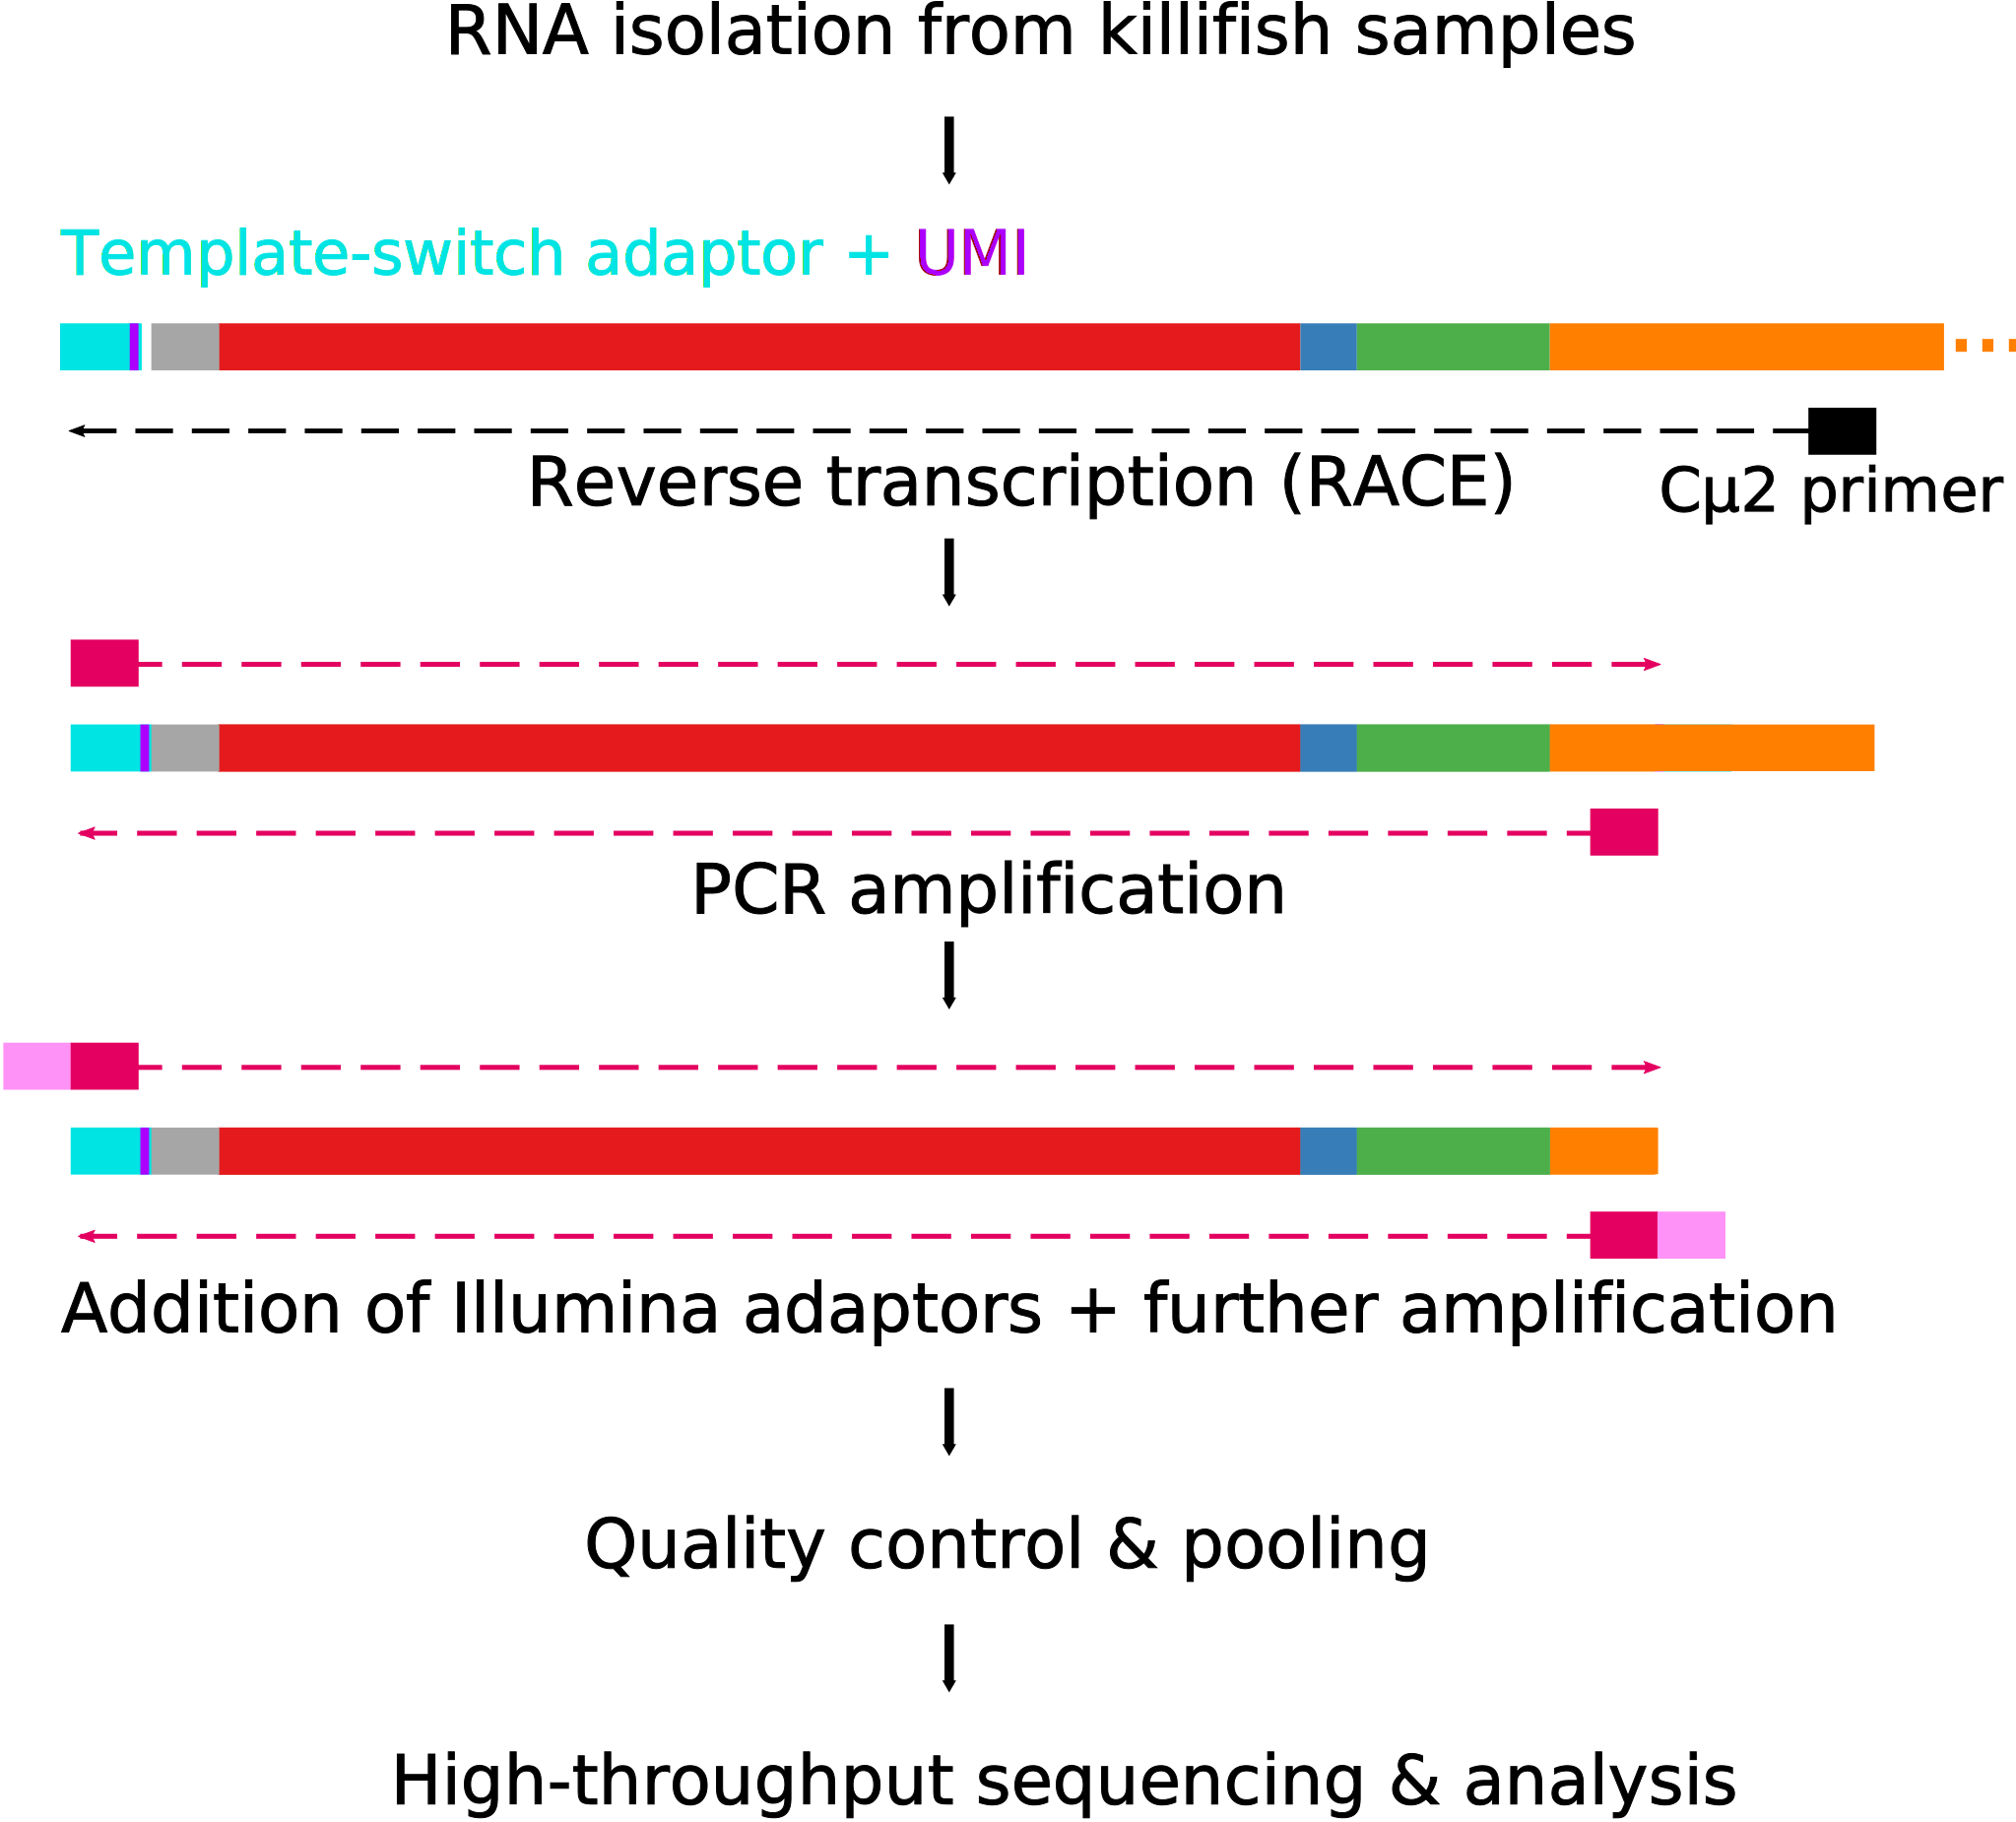
\includegraphics[width=0.7\textwidth]{output_files/figures/pdf/igseq-igrace-pipeline}
\Caption{Summary of the \igseq library-preparation protocol for turquoise-killifish samples}{Schematic summary of library-preparation protocol used to prepare immunoglobulin-sequencing libraries from turquoise-killifish samples. In order to capture all \igh{M} transcripts (both secreted and transmembrane), the reverse-transcription primer was homologous to the \cm{2} exon, while the PCR primers were homologous to \cm{1}. The third step (``Addition of Illumina adapters + further amplification'') represents two distinct rounds of PCR amplification and bead purification, for stepwise addition of Illumina TruSeq adapter sequences.}
\label{fig:igrace-pipeline}
\vspace{0.5em}
\end{figure}

Following reverse transcription, the reaction mixture is treated with uracil-DNA glycosylase (UDG) to specifically remove residual TSAs through digestion of deoxyuridine residues (which are absent in the template sequence). The library then undergoes three successive rounds of PCR amplification (\Cref{fig:igrace-pipeline}, \Cref{sec:methods_molec_igseq_pcr}), which respectively serve to amplify the reverse-transcribed cDNA sequence; amplify further while adding partial Illumina TruSeq adapter sequences; and add complete adapter sequences including library-specific P1 and P2 index sequences \parencite{vollmers2013consensus}. In the first two cases, the PCR primer sequences are homologous to the invariant part of the TSA sequence and the \cm{1} exon, respectively; as all known forms of \igh{} in turquoise killifish (\igh{M-TM}, \igh{M-S} and \igh{D-TM}) share this exon, the isotype- and isoform-specificity of the library prep can be altered simply by changing the position of the reverse-transcription GSP, with all other primer sequences left unchanged. In all experiments included in this chapter, a GSP on the \cm{2} exon was used, resulting in a library including \igh{M-TM} and \igh{M-S} sequences but excluding \igh{D}.

Libraries to be sequenced together are then pooled in equimolar ratio and the pooled sample undergoes size-selection to remove residual primer-dimers and other unwanted sequences (\Cref{sec:methods_molec_igseq_seq}). The complete library-preparation protocol reliably produces a single peak in the range of 650-\bp{680}, consistent with the known lengths of \vh, \dh and \jh gene segments in the \Nfu locus. Following size-selection and quality control, pooled libraries are sequenced on an Illumina MiSeq sequencing machine with 2$\times$\bp{300} reads (\Cref{sec:methods_molec_igseq_seq}); this longer read length is necessary to completely cover the variable region. To avoid problems associated with the low sequence complexity of single-amplicon sequencing libraries \parencite{illumina2017diversity}, a large proportion of PhiX spike-in (30\,\%) was used to increase the sequence complexity of the libraries.

\subsection{Sequence pre-processing with \program{pRESTO}}
\label{sec:igseq_protocol_preprocess}

\begin{figure}
\centering
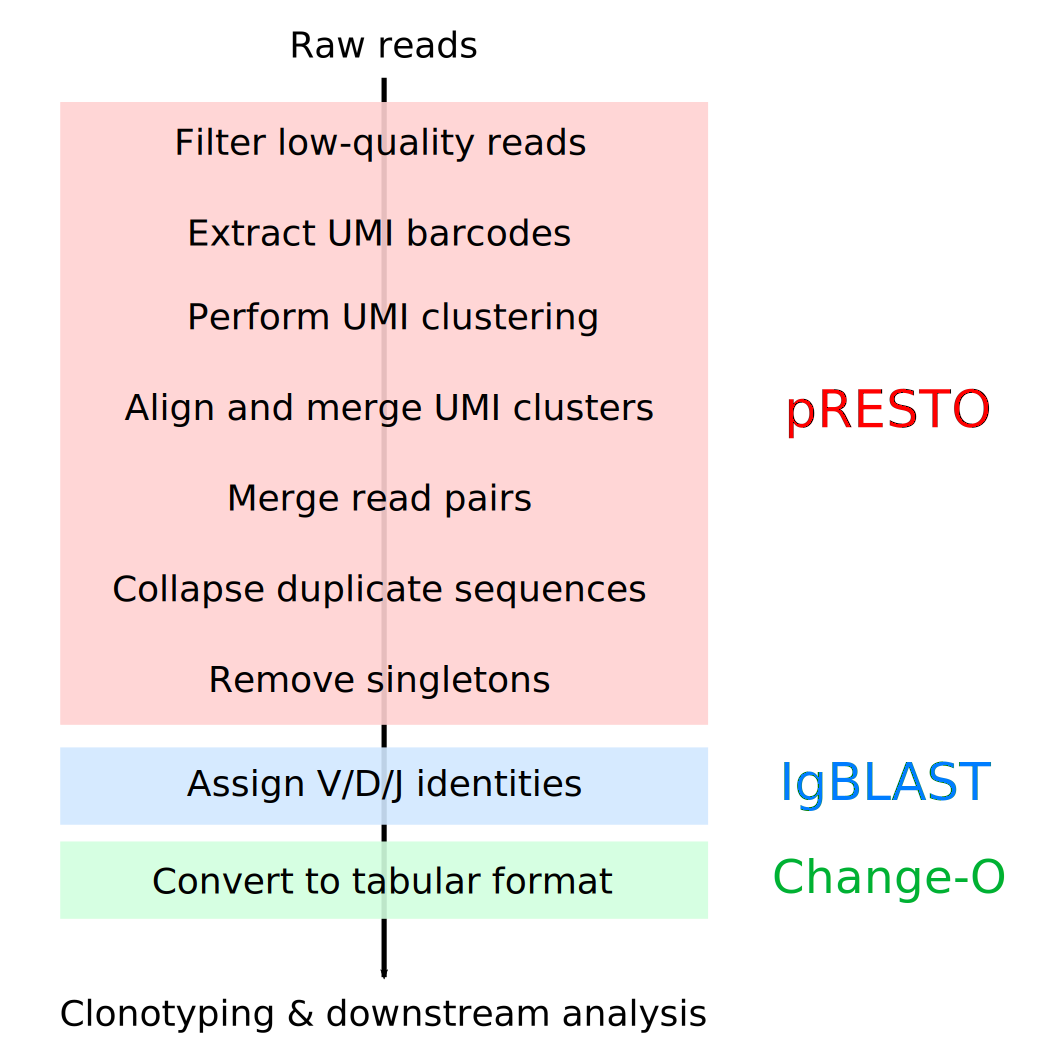
\includegraphics[width=0.6\textwidth]{output_files/figures/pdf/igseq-preprocessing}
\Caption{Summary of the \igseq pre-processing pipeline for turquoise-killifish data}{Schematic summary of post-sequencing analysis pipeline of killifish \igseq data, up to and including conversion from \format{FASTA} to \program{Change-O} tabular format. Clonotyping and additional downstream analysis methods are described in \Cref{sec:igseq_pilot,sec:methods_comp_igpreproc_clones,sec:methods_comp_igpreproc_clones}.}
\label{fig:igrace-preprocessing}
\vspace{0.5em}
\end{figure}

Raw \igseq data from the protocol described in \Cref{sec:igseq_protocol_library} takes the form of a large number of paired-end sequencing reads, each of which represents a single biased and error-prone observation from the set of input sequences in the original sample. To get from this fragmented and unreliable dataset to a set of complete, error-corrected and bias-adjusted \igh{} variable-region sequences, extensive pre-processing (\Cref{sec:methods_comp_igpreproc}) must be performed on the raw data. In this case, this pre-processing was largely carried out with \program{pRESTO} \parencite{vanderheiden2014presto}, part of the Immcantation suite of repertoire-sequencing analysis tools (\Cref{fig:igrace-preprocessing}).

To begin with, each read pair in the dataset is annotated with various information about the source individual (ID, strain, sex, age and weight at death, etc.) as well as information about its place in the replicate structure of the experiment (\Cref{sec:methods_comp_igpreproc_annot}). The sequences are then filtered to remove low-quality sequences (with a mean Phred score of less than 20 \parencite{ewing1998phred}). Invariant primer sequences are trimmed from the ends of the reads, and the UMI sequence of each forward read (containing the TSA sequence) is extracted into a sequence annotation and trimmed from the read sequence (\Cref{sec:methods_comp_igpreproc_mask}).

As discussed in \Cref{sec:igseq_protocol_library}, the use of UMI sequences enables biases and errors in library insert sequences to be corrected by taking the consensus sequence of all reads sharing a given UMI. However, PCR and sequencing errors can also affect the sequence of the UMI itself, in which case reads that in fact belong to a single group will be spuriously separated during pre-processing; this can result in spuriously low UMI group sizes, spuriously high numbers of unique sequences, and avoidable loss of sequencing data due to reads with erroneous barcodes being discarded (as low-quality, low-read-count unique sequences) at various points in the pre-processing pipeline \parencite{shlemov2017igrec}. In addition to these barcode \textit{errors}, barcode \textit{collisions} can occur, in which multiple distinct sequences are labelled with the same UMI sequence and spuriously grouped together during UMI grouping. This can lead to spuriously large UMI groups and spuriously low numbers of unique sequences, and in extreme cases can lead to the rejection and loss of entire UMI groups due to an insufficiently high level of internal sequence identity during consensus-read generation \parencite{shlemov2017igrec}.

In order to reduce the effect of such barcode errors and collisions on the pre-processing pipeline, primer-trimmed forward reads in this pipeline undergo clustering following extraction of UMI sequences (\Cref{sec:methods_comp_igpreproc_correct}). Firstly, reads are clustered by UMI sequence, and those with sufficiently similar UMIs are grouped together into a single cluster even if their UMIs differ slightly. Following this, the insert sequences (as opposed to UMI sequences) of the reads in each cluster are themselves clustered, and those with sufficiently different insert sequences are split apart into separate clusters. Following these clustering steps, each cluster consists of reads with highly similar barcode sequences as well as similar insert sequences; it is then these clusters, rather than the raw UMI sequences, on which consensus-read generation is performed.

Following cluster inference as described above, annotations (including barcode and cluster annotations) are copied from each TSA-bearing forward-read to its mate among the reverse reads. The forward and reverse reads were then separately grouped by cluster identity and collapsed into a consensus sequence (\Cref{sec:methods_comp_igpreproc_consensus}), based on the quality score of each aligned base call at each position \parencite{vanderheiden2014presto}. As most PCR and sequencing errors should be present in only a minority of the sequences descended from a given input sequence, this process effectively corrects these errors, while also removing the effect of biased amplification on observed sequence abundance. The more sequences present in a given cluster, the more effective is consensus-read generation at correcting these errors; as such, when sequencing \igseq libraries there is a trade-off inherent in the amount of oversequencing of the molecules in each library, with more reads per molecule improving error correction but reducing the amount of useful information gained per sequencing read \parencite{turchaninova2016igprep}.

Following consensus-read generation, pairs of forward and reverse consensus reads with matching cluster annotations are assembled into a single contiguous sequence, ideally covering the entire variable-region sequence of the template molecule (\Cref{sec:methods_comp_igpreproc_collapse}); forward or reverse consensus reads lacking a mate in the other read set are discarded. At this point in the pipeline, each entry is assumed to represent a distinct RNA template molecule in the original sample. Sequences with different cluster annotations but matching insert sequences are then collapsed together into a single sequence, which is annotated with the number of contributing consensus reads (\Cref{sec:methods_comp_igpreproc_collapse}); each sequence entry now represents a unique sequence in the dataset. Finally, unique sequences represented by only a single read pair (which could not be corrected by consensus-read generation and are therefore highly unreliable) are discarded.

At the end of the \program{pRESTO} pre-processing pipeline, the raw data has been processed into a set of complete variable-region sequences, each of which is annotated with the number of contributing reads and the number of distinct instances of that sequence found in the dataset. These sequences are then assigned V/D/J-identities through alignment to reference databases with \program{IgBLAST} (\Cref{sec:methods_comp_igpreproc_igblast}) \parencite{ye2013igblast}. Finally, the sequences and their metadata, including annotations and V/D/J-identities, are converted by \program{Change-O} (another program from the Immcantation suite) \parencite{gupta2015changeo} into tabular format for efficient downstream processing and analysis (\Cref{fig:igrace-preprocessing}).

\FloatBarrier
\clearpage

\section{Establishing \igseq in the turquoise killifish: pilot study}
\label{sec:igseq_pilot}

In order to refine and functionally validate the library-preparation protocol and processing pipeline described in \Cref{sec:igseq_protocol}, as well as assess the state of the turquoise-killifish antibody repertoire in mature adults, I selected a group of four killifish from the second, eight-week-old sample group (specifically, fish 2-03, 2-04, 2-05 and 2-06 from \Cref{tab:igseq-cohorts-fish}) for a pilot study. In this experiment, total RNA was isolated twice independently from each fish, and independent library preps were performed once on the first RNA isolate and twice on the second, for a total of three replicates per individual (\Cref{fig:igseq-pilot-design}). These twelve replicates were sequenced together in a single MiSeq run, yielding a total of \embed{output_files/txt/igseq-pilot-nreads-raw-total.txt} million read pairs (\embed{output_files/txt/igseq-pilot-nreads-raw-replicate-min.txt} to \embed{output_files/txt/igseq-pilot-nreads-raw-replicate-max.txt} million pairs per replicate, \embed{output_files/txt/igseq-pilot-nreads-raw-individual-min.txt} to \embed{output_files/txt/igseq-pilot-nreads-raw-individual-max.txt} million pairs per individual). These data were then used to develop the downstream analysis pipeline for killifish immunoglobulin-sequencing data, validate the performance and replicability of the protocol, and investigate the state of the antibody repertoire in mature adult killifish.

\begin{figure}
\centering
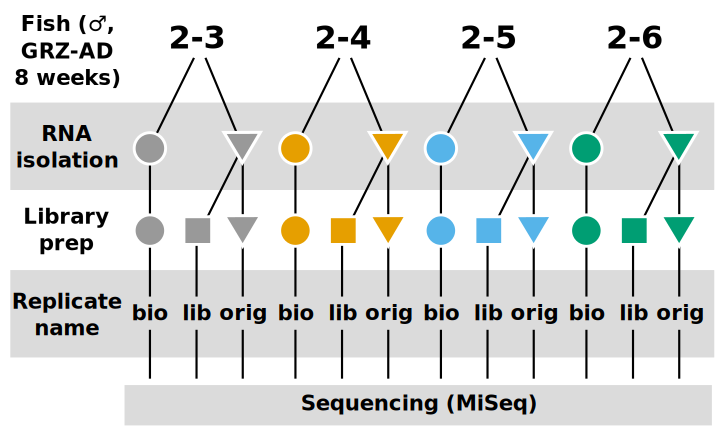
\includegraphics[width = 0.9\textwidth]{output_files/figures/pdf/igseq-pilot-design}
\caption[Experimental design of killifish \igseq pilot study]{\textbf{Experimental design of killifish \igseq pilot study}, showing relationship between replicates for each individual. Colour denotes individual of origin, while shape denotes replicate type.}
\label{fig:igseq-pilot-design}
\end{figure}

\subsection{Read survival and composition}
\label{sec:igseq_pilot_composition}

\Cref{fig:igseq-pilot-read-survival-init} shows the absolute and relative read survival for each of the twelve replicates throughout the pre-processing pipeline, up to and including VDJ assignment and Change-O table construction. The twelve replicates show relatively consistent behaviour, with \embed{output_files/txt/igseq-pilot-read-survival-init-min.txt}\,\% to \embed{output_files/txt/igseq-pilot-read-survival-init-max.txt}\,\% of reads surviving the entire process. Of those that do not, the biggest losses typically occur during quality filtering and removal of singleton sequences, with most other steps giving rise to relatively little sequence loss (\Cref{fig:igseq-pilot-read-survival-init-b}).

\begin{figure}
\centering
\includegraphics[width = 0.9\textwidth]{output_files/figures/pdf/igseq-pilot-read-survival-init}
\begin{subfigure}{0em}
\phantomsubcaption{}
\label{fig:igseq-pilot-read-survival-init-a}
\end{subfigure}
\begin{subfigure}{0em}
\phantomsubcaption{}
\label{fig:igseq-pilot-read-survival-init-b}
\end{subfigure}
\Caption{Read survival during initial pre-processing of the \igseq pilot dataset}{Line graphs of absolute (A) and relative (B) read survival during pre-processing of the \igseq pilot dataset, up to VDJ assignment and Change-O table construction.}
\label{fig:igseq-pilot-read-survival-init}
\end{figure}

In total, the pre-processed sequence repertoires of the pilot replicates contain between \embed{output_files/txt/igseq-pilot-nseq-init-replicate-min.txt} and \embed{output_files/txt/igseq-pilot-nseq-init-replicate-max.txt} unique sequences per replicate, corresponding to between \embed{output_files/txt/igseq-pilot-nseq-init-individual-min.txt} and \embed{output_files/txt/igseq-pilot-nseq-init-individual-max.txt} unique sequences per individual killifish and \embed{output_files/txt/igseq-pilot-nseq-init-total.txt} unique sequences in total. Of these, \embed{output_files/txt/igseq-pilot-nseq-init-pc-functional.txt}\,\% of sequences (corresponding to \embed{output_files/txt/igseq-pilot-nreads-init-pc-functional.txt}\,\% of surviving sequencing reads) are annotated by \program{Change-O} as functional, meaning they have successfully been assigned V- and J-identities, their V- and J-sequences are in-frame, and they do not contain any stop codons (\Cref{fig:igseq-pilot-functional-prop-a}). A further \embed{output_files/txt/igseq-pilot-nseq-init-pc-noj.txt}\,\% of sequences (corresponding to \embed{output_files/txt/igseq-pilot-nreads-init-pc-noj.txt}\,\% of surviving reads) failed to be assigned even an uncertain J-identity, meaning that no \jh sequence in the reference database aligned to the insert sequence; the remaining \embed{output_files/txt/igseq-pilot-nseq-init-pc-other.txt}\,\% of sequences (corresponding to \embed{output_files/txt/igseq-pilot-nreads-init-pc-other.txt}\,\% of surviving reads) have a J-assignment but are rendered nonfunctional by an internal stop codon and/or a frameshift between their V- and J-sequences (\Cref{fig:igseq-pilot-functional-prop-a}), arising during primary diversification (\Cref{sec:intro_immunity_primary}) or possibly SHM.

\begin{figure}
\centering
\includegraphics[width = 0.9\textwidth]{output_files/figures/pdf/igseq-pilot-functional-prop}
\begin{subfigure}{0em}
\phantomsubcaption{}
\label{fig:igseq-pilot-functional-prop-a}
\end{subfigure}
\begin{subfigure}{0em}
\phantomsubcaption{}
\label{fig:igseq-pilot-functional-prop-b}
\end{subfigure}
\Caption{Functional composition and V-score filtering in the \igseq pilot dataset}{Proportion of input reads, UMI groups and unique sequences in the \igseq pilot dataset belonging to different (non)functional categories, before (A) and after (B) filtering on V-alignment score.}
\label{fig:igseq-pilot-functional-prop}
\end{figure}

As genuinely rearranged but nonfunctional sequences would be expected to have undergone V(D)J recombination and so have a complete J-sequence, the lack of assigned J-identities for a significant minority of sequences suggests that this subset of sequences may be artefactual, erroneous or otherwise malformed. Supporting this assumption, sequences without J-assignments overwhelmingly have very low V-alignment scores reported by \program{IgBLAST}, with an average score of \embed{output_files/txt/igseq-pilot-vscore-mean-noj.txt} $\pm$ \embed{output_files/txt/igseq-pilot-vscore-sd-noj.txt} (mean $\pm$ standard deviation), compared to \embed{output_files/txt/igseq-pilot-vscore-mean-other.txt} $\pm$ \embed{output_files/txt/igseq-pilot-vscore-sd-other.txt} for other nonfunctional sequences and \embed{output_files/txt/igseq-pilot-vscore-mean-functional.txt} $\pm$ \embed{output_files/txt/igseq-pilot-vscore-sd-functional.txt} for functional sequences (\Cref{fig:igseq-pilot-functional-vscores}). A simple V-score cut-off of 100, therefore, effectively removes the vast majority of these low-quality sequences, while leaving the population of functional sequences intact (\Cref{fig:igseq-pilot-functional-prop-b}).

\begin{figure}
\centering
\includegraphics[width = 0.9\textwidth]{output_files/figures/pdf/igseq-pilot-functional-vscores}
\Caption{V-score distributions of functional and nonfunctional sequences}{Kernel density plots of distributions of V-alignment scores among unique sequences in the \igseq pilot dataset. Vertical axes are not to scale between sequence categories.}
\label{fig:igseq-pilot-functional-vscores}
\end{figure}

In total, \embed{output_files/txt/igseq-pilot-nseq-init-dropped-vscore.txt} unique sequences, corresponding to \embed{output_files/txt/igseq-ageing-rel-loss-total.txt}\,\% of input reads, were removed in this way. As a result, including this final filtering step, between \embed{output_files/txt/igseq-pilot-read-survival-all-min.txt}\,\% and \embed{output_files/txt/igseq-pilot-read-survival-all-max.txt}\,\% of reads per input library survived up to this point in the pipeline (\Cref{fig:igseq-pilot-read-survival-all}), a good range suggesting both that the library-preparation protocol successfully captured antibody-repertoire sequencing data from turquoise killifish for the first time, and that the subsequent computational pipeline was able to completely and successfully process the majority of the resulting data. Of the remaining \embed{output_files/txt/igseq-pilot-nseq-init-kept-vscore.txt} unique sequences present in the dataset, \embed{output_files/txt/igseq-pilot-nseq-init-functional-filtered.txt} (\embed{output_files/txt/igseq-pilot-nseq-init-pc-functional-filtered.txt}\,\%) are functional, \embed{output_files/txt/igseq-pilot-nseq-init-other-filtered.txt} (\embed{output_files/txt/igseq-pilot-nseq-init-pc-other-filtered.txt}\,\%) are rendered nonfunctional by a stop codon or frameshift, and only \embed{output_files/txt/igseq-pilot-nseq-init-noj-filtered.txt} (\embed{output_files/txt/igseq-pilot-nseq-init-pc-noj-filtered.txt}\,\%) could not be assigned a J-identity (\Cref{fig:igseq-pilot-functional-prop-b}). These results confirm that the data from this first \igseq experiment in the turquoise killifish are of sufficient quality to proceed to clonotyping and analysis of repertoire diversity.

\subsection{Clonotyping and clonal repertoire diversity}
\label{sec:igseq_pilot_clones}

Following assignment of VDJ identities and quality filtering, sequences in an antibody repertoire can be assigned to clones: groups of B-cells descended from a single \naive B-cell ancestor, and therefore sharing a single VDJ-recombination event. Sequences in the same clone are said to share a \textit{clonotype}. In \program{Change-O}, clonotyping is performed by dividing sequences into groups sharing a consistent V-assignment, J-assignment and CDR3 length, then performing single-linkage clustering on each group of sequences based on Hamming distances between CDR3 sequences \parencite{gupta2017hierarchical}. To identify a distance threshold for cutting the cluster dendrogram into clones, each unique sequence in the repertoire is assigned a nearest-neighbour distance based on the length-normalised Hamming distance to the most similar sequence in the repertoire. The resulting nearest-neighbour distribution is typically bimodal, with the lower peak (representing more-similar sequences) indicating members of the same clonotype and the higher peak (representing less-similar sequences) indicating members of different clones; by fitting a pair of gamma or normal distributions to these two peaks, a distance threshold for clonotype membership can be determined according to the desired levels of sensitivity and specificity \parencite{nouri2018threshold} (\Cref{sec:methods_comp_igpreproc_clones}). By cutting the cluster dendrogram at this threshold, each group of repertoire sequences can be separated into some number of distinct clones, each of which is assumed to share a unique \naive B-cell ancestor.

One disadvantage of single-linkage clustering in this context is that non-informative \sequence{N} positions can result in artifactual links between unrelated sequences. As such, sequences with a large number of junctional \sequence{N} positions can significantly disrupt the clonotyping process. On the other hand, as over \embed{output_files/txt/igseq-pilot-filtered-nn-any.txt}\,\% of unique sequences in the pilot dataset contain at least one such junctional \sequence{N} position, excluding them all would represent a significant loss of data. In order to minimise the number of discarded sequences while also minimising the disrupting effects of sequences with junctional \sequence{N}s, sequences with exactly one junctional \sequence{N} position (comprising \embed{output_files/txt/igseq-pilot-filtered-1n-total.txt}\,\% of total sequences and \embed{output_files/txt/igseq-pilot-filtered-1n-withn.txt}\,\% of sequences with at least one junctional \sequence{N}; \Cref{tab:igseq-pilot-filtered-nn}) were included in the clonotyping process for the pilot dataset, while those with two or more junctional \sequence{N} positions were excluded. This procedure successfully assigned clonal identities to \embed{output_files/txt/igseq-pilot-nseq-assigned-clones.txt}\,\% of unique sequences in the V-score-filtered dataset, with fewer than \embed{output_files/txt/igseq-pilot-nseq-lost-clonotyping.txt} sequences (corresponding to \embed{output_files/txt/igseq-pilot-pc-reads-lost-clonotyping.txt}\,\% of input reads) lost during the clonotyping phase of the pipeline.

\begin{table}
\caption{Distribution of junctional \sequence{N} positions in the V-score-filtered pilot dataset}
\label{tab:igseq-pilot-filtered-nn}
% latex table generated in R 3.5.2 by xtable 1.8-3 package
% Wed Apr  3 14:27:33 2019
\begin{tabular}{lrrr}
  \toprule \# junctional Ns & \# unique sequences & \% of all sequences & \% of sequences with $>$0 junctional Ns \\ 
  \midrule 0 & 49134 & 88.924 & 0.00 \\ 
  1 & 3388 & 6.132 & 67.94 \\ 
  2 & 961 & 1.739 & 19.27 \\ 
  3 & 324 & 0.586 & 6.50 \\ 
  4 & 125 & 0.226 & 2.51 \\ 
  5 & 93 & 0.168 & 1.86 \\ 
  $>$5 & 96 & 0.174 & 1.93 \\ 
   \bottomrule \end{tabular}

\end{table}

In total, \embed{output_files/txt/igseq-pilot-nclones-individual-min.txt} to \embed{output_files/txt/igseq-pilot-nclones-individual-max.txt} clones were identified per individual fish in the pilot dataset. As expected, the clone-size distribution is overwhelmingly dominated by small clones (\Cref{fig:igseq-pilot-clone-sizes-sizes}): across all individuals, \embed{output_files/txt/igseq-pilot-nclones-pc-1count.txt}\,\% of clones are observed as just a single unique sequence across all replicates, while \embed{output_files/txt/igseq-pilot-nclones-pc-small.txt}\,\% contain fewer than five unique sequences. As a result, the great majority of clones (\embed{output_files/txt/igseq-pilot-nclones-pc-1rep.txt}\,\%) are observed in only a single replicate per individual, with \embed{output_files/txt/igseq-pilot-nclones-pc-2rep.txt}\,\% present in two replicates and only \embed{output_files/txt/igseq-pilot-nclones-pc-1rep.txt}\,\% shared across all three. Unsurprisingly, however, larger clones are much more likely to be shared across multiple replicates (\Cref{fig:igseq-pilot-clone-sizes-reps}), consistent with a model in which a very large number of small clones are sampled only rarely while a much smaller number of large clones is sampled much more often \parencite{mora2016diversity}. Overall, the level of agreement between the replicates is high (\Cref{fig:igseq-pilot-clone-sizes-cor}), with an average inter-replicate correlation in clone size of $r=\embed{output_files/txt/igseq-pilot-clones-interrep-cor-avg.txt}$, indicating that, despite the problem of undersampling many very small clones, the clonal composition of the killifish can be captured reproducibly by \Igseq.

\begin{figure}
\centering
\includegraphics[width = 0.9\textwidth]{output_files/figures/pdf/igseq-pilot-clone-sizes}
\begin{subfigure}{0em}
\phantomsubcaption{}
\label{fig:igseq-pilot-clone-sizes-sizes}
\end{subfigure}
\begin{subfigure}{0em}
\phantomsubcaption{}
\label{fig:igseq-pilot-clone-sizes-reps}
\end{subfigure}
\Caption{Clone size and cross-replicate reproducibility in the \igseq pilot dataset}{(A) Proportion of clones of different sizes for each individual in the pilot dataset, measured in unique sequences per clone. (B) LOESS-smoothed curves \parencite{cleveland1991loess} showing proportion of clones of each size found across one, two or all three replicates of the appropriate individual.}
\label{fig:igseq-pilot-clone-sizes}
\end{figure}

\begin{figure}
\centering
\includegraphics[width = 0.75\textwidth]{output_files/figures/pdf/igseq-pilot-clone-sizes-cor}
\begin{subfigure}{0em}
\phantomsubcaption{}
\label{fig:igseq-pilot-clone-sizes-cor-boxplots}
\end{subfigure}
\begin{subfigure}{0em}
\phantomsubcaption{}
\label{fig:igseq-pilot-clone-sizes-cor-scatter}
\end{subfigure}
\Caption{Clone-size correlation between pilot replicates}{(A) Boxplots showing distribution of Pearson product-moment correlation coefficients of clone sizes for each pair of replicates, as measured by the number of unique sequences per clone in each replicate. (B) Scatter plots comparing clone sizes across biological replicates for each individual in the pilot dataset. In both subfigures, clones absent in a given replicate were given a size of zero.}
\label{fig:igseq-pilot-clone-sizes-cor}
\end{figure}

One of the most strikingly reproducible findings of immune-repertoire-sequencing studies has been the approximately power-law distribution of the clonal repertoire, a phenomenon observed in both antibody and TCR repertoires across multiple different species \parencite{desponds2016fluctuating,mora2016diversity}. More precisely, the frequency of the $k$th largest clone in a repertoire dataset containing $N$ total clones can often be roughly predicted by a Zipf distribution \parencite{mora2010mentropy} of the form:

\begin{equation}
f(k | N, s) = \frac{k^{-s}}{H_{N,s}}
\end{equation}

\noindent for some exponent parameter $s > 0$, where $H_{N,s}$ is the $N$th generalised harmonic number of order $s$ (\Cref{sec:methods_comp_igdownstream_zipf}). This power-law distribution of clone sizes is inconsistent with clonal expansion under neutral selection and instead suggests that clone sizes evolve within a complex and fluctuating fitness landscape \parencite{desponds2016fluctuating}. Before going on with more detailed investigation of the diversity structure of turquoise killifish antibody repertoires, it would be interesting to test whether the phenomenon of roughly Zipf-distributed clonal frequencies persists in this species as well.

\Cref{fig:igseq-pilot-clones-zipf-lines} shows the rank/frequency distributions of the clonal repertoires of the four individuals from the pilot dataset. From roughly the tenth-largest clone onwards, these distributions appear approximately linear on a log-log plot and can be reasonably approximated by a power-law distribution; however, the largest clones in each repertoire clearly deviate from this pattern, and are much larger than would be predicted by a power-law approximation. In order to fit power-law curves to these distributions, I performed simple maximum-likelihood estimation of the Zipf exponent for each individual repertoire in \program{R} (\Cref{sec:methods_comp_igdownstream_zipf}). When the five largest clones in each repertoire were excluded from the calculation, the resulting Zipf distributions (\Cref{fig:igseq-pilot-clones-zipf-fit}) provided a good approximation of the remaining points and were highly consistent across individuals, with exponents ranging from \embed{output_files/txt/igseq-pilot-clone-zipf-exp-min.txt} to \embed{output_files/txt/igseq-pilot-clone-zipf-exp-max.txt}. Conversely, when the largest clones are included, the resulting Zipf approximations follow the line of the remaining clones much less accurately in several individuals, and their exponents range more widely from \embed{output_files/txt/igseq-pilot-clone-zipf-exp-null-min.txt} to \embed{output_files/txt/igseq-pilot-clone-zipf-exp-null-max.txt}. Hence, while the bulk of the clonal repertoire in turquoise killifish corresponds to the expected power-law behaviour seen in other species, the largest clones, for unknown reasons, consistently deviate strongly from this pattern.

\begin{figure}
\centering
\includegraphics[width=0.8\textwidth]{output_files/figures/pdf/igseq-pilot-clone-zipf-lines}
\Caption{Rank/frequency distributions of pilot clonal repertoires}{Log-log line plots of rank/frequency distributions of the individual clonal repertoires in the \igseq pilot dataset, showing the roughly linear (i.e. power-law-distributed) distribution of smaller clones (roughly rank 10 onwards) and the clear deviation from this distribution in the largest clones.}
\label{fig:igseq-pilot-clones-zipf-lines}
\end{figure}

\begin{figure}
\centering
\includegraphics[width=0.7\textwidth]{output_files/figures/pdf/igseq-pilot-clone-zipf-grad}
\begin{subfigure}{0em}
\phantomsubcaption{}
\label{fig:igseq-pilot-clones-zipf-fit}
\end{subfigure}
\begin{subfigure}{0em}
\phantomsubcaption{}
\label{fig:igseq-pilot-clones-zipf-fit-null}
\end{subfigure}
\Caption{Best-fit Zipf distributions of pilot clonal repertoires}{Log-log scatter plots of the rank/frequency distributions for each clonal repertoire in the pilot dataset, overlaid with a maximum-likelihood estimate of the underlying Zipf distribution computed (A) with the five largest clones excluded or (B) with all clones included. In (A), the clones excluded from the Zipf estimation are plotted as crosses.}
\label{fig:igseq-pilot-clones-zipf-fit-grid}
\end{figure}

In addition to the exponent of the best-fit Zipf distribution, another quick and simple way to measure the extent to which a clonal repertoire is dominated by the largest clones is to measure the P20, the proportion of all unique sequences in the repertoire belonging to the 20 largest clones; in humans, for example, the P20 is typically a few percent in healthy individuals, but can reach up to 90\,\% in patients with B-cell malignancies \parencite{rosenfeld2018clonesize}. In the killifish pilot dataset, the P20 of the clonal repertoires ranges from \embed{output_files/txt/igseq-pilot-clone-zipf-p20-obs-min.txt}\,\% to \embed{output_files/txt/igseq-pilot-clone-zipf-p20-obs-max.txt}\,\% (\Cref{fig:igseq-pilot-clones-zipf-p20}), much higher than that observed in healthy humans. These high P20 values are primarily due to the highly expanded state of the largest few clones in each repertoire; when the expected clonal frequencies from the Zipf distributions fitted in \Cref{fig:igseq-pilot-clones-zipf-fit} are used instead of the actual values, the P20 values fall to between \embed{output_files/txt/igseq-pilot-clone-zipf-p20-exp-min.txt}\,\% and \embed{output_files/txt/igseq-pilot-clone-zipf-p20-exp-max.txt}\,\% (\Cref{fig:igseq-pilot-clones-zipf-p20}).

\begin{figure}
\centering
\includegraphics[width=0.8\textwidth]{output_files/figures/pdf/igseq-pilot-clone-p20}
\Caption{Clonal P20 values in \Nfu pilot repertoires}{(A) Boxplots of observed and expected (from the Zipf distributions fitted in \Cref{fig:igseq-pilot-clones-zipf-fit}) P20 distributions of the clonal repertoires from the \igseq pilot dataset. Pairwise $p$-value computed using nonparametric Mann-Whitney $U$ test ($*: 0.01 < p \leq 0.05;~**: 0.001 < p \leq 0.01;~***: p \leq 0.001$) . (B) Scatter plot comparing observed vs expected P20 for each individual, annotated with the correlation ($r$) between the two sets of P20 values.}
\label{fig:igseq-pilot-clones-zipf-p20}
\end{figure}

In addition to investigating the P20, Rosenfeld \textit{et al.} \parencite{rosenfeld2018clonesize} recommend evaluating clonal expansions in antibody repertoires on the basis of both the relative clonal frequency of the largest clones in the repertoire and the extent to which each such clone is larger than the next-largest clone, with recommended cutoffs for human data of 5\,\% for the former and threefold for the latter. In the pilot killifish dataset, clones exceeding 5\,\% of unique sequences in the repertoire occur in three out of four individuals (2-03, 2-04 and 2-06), while clones exceeding the size of the next-largest clone by at least threefold occur in a different three individuals (2-03, 2-05 and 2-06). However, only one individual, 2-04, exhibits a potentially medically-relevant clonal expansion by the standards of Rosenfeld \textit{et al.}; this clone (2-04\_8143) occupies 6.8\,\% of the repertoire and is roughly 3.1-fold larger than the next-largest clone, and is identified reproducibly as a clonal expansion in both the pooled dataset (\Cref{fig:igseq-pilot-clones-expansions}) and each of the separate replicates (\Cref{fig:igseq-pilot-clones-expansions-rep}) from individual 3-04. These results could be taken as demonstrating that potentially medically-relevant clonal expansions are present, albeit not common, in middle-aged adult male turquoise killifish; however, without functional validation it is not clear to what extent the recommended guidelines derived from human data apply to this species, especially when the body size (and hence the potential clonal richness) of turquoise killifish is so much smaller.

\begin{figure}
\centering
\includegraphics[width=0.8\textwidth]{output_files/figures/pdf/igseq-pilot-clone-expansions}
\Caption{Clonal expansions in \Nfu pilot repertoires}{Scatter plots of clonal abundance for each individual in the \igseq pilot dataset, measured in terms of the proportion of unique sequences in the repertoire ($x$-axis) and the abundance relative to the next-largest clone ($y$-axis). Thresholds for identifying clonal expansions (5\,\% and 3-fold for the $x$- and $y$-axis, respectively) suggested by Rosenfeld \textit{et al.} \parencite{rosenfeld2018clonesize}.}
\label{fig:igseq-pilot-clones-expansions}
\end{figure}

Having investigated the clonal abundance distribution and various measures of clonal expansion, we now come to the question of the \textit{diversity} of the killifish clonal repertoire. As discussed in detail in \Cref{app:diversity}, the diversity of a population can be interpreted -- and measured -- in multiple ways, with different measures laying different amounts of emphasis on the richness (number of species) and evenness (relative distribution of species) of that population and giving different degrees of consideration to common vs rare species (\Cref{app:diversity-unitary-simple}). In order to visualise many different aspects of repertoire diversity simultaneously and on a common scale, Hill diversity spectra \parencite{hill1973diversity} can be used. For any population $X$ of elements (or \textit{individuals}) divisible into some disjoint set of categories (or \textit{species}) $S$, the \textit{Hill numbers} or ``true diversities'' of that population (\Cref{app:diversity-unitary-hill}) \parencite{hill1973diversity, jost2006entropy} are given by

\begin{equation}
^qD(X) = \begin{cases} \left(\displaystyle\sum_{s \in S} p_s^q \right)^{\frac{1}{1-q}} & q \neq 1\\
\exp\left(-\displaystyle\sum_{s \in S}p_s \cdot \ln p_s\right) & q = 1 \end{cases}
\end{equation}

\noindent where $p_s$ is the proportion of individuals in $X$ belonging to a species $s$. The parameter $q$ in this equation denotes the \textit{order} of diversity: the greater the order, the more rare species are downweighted compared to common ones when computing the diversity of the population. By plotting $^qD$ as a function of $q$ across a wide range of diversity orders, we can therefore observe how the measured diversity of the population changes as we put progressively more or less emphasis on species of different abundances, and so simultaneously visualise many different aspects of population diversity (\Cref{app:diversity-unitary-hill,app:diversity-structured-calc}).

\Cref{fig:igseq-pilot-clone-diversity} shows the diversity of clone sizes in each individual in the pilot dataset, as measured using Hill diversity spectra across each individual's three replicates (\Cref{fig:igseq-pilot-design}). \Cref{fig:igseq-pilot-clone-diversity-alpha} gives the alpha diversity, or average \textit{within-replicate} diversity, while \Cref{fig:igseq-pilot-clone-diversity-beta} shows the beta diversity, or variation in clone-size distribution \textit{between replicates} for each individual (\Cref{app:diversity-structured-terminology,app:diversity-structured-calc}). In both cases, each curve represents a single individual and gives the corresponding diversity measure at a range of different diversity orders. As beta diversity (unlike alpha diversity) is sensitive to the number of sub-populations being compared, it has been rescaled here such that 0 represents the minimum possible beta diversity at each order and 1 represents the maximum (\Cref{app:diversity-structured-rescaling}).

\begin{figure}
\centering
\includegraphics[width = 0.9\textwidth]{output_files/figures/pdf/igseq-pilot-clone-diversity}
\begin{subfigure}{0em}
\phantomsubcaption{}
\label{fig:igseq-pilot-clone-diversity-alpha}
\end{subfigure}
\begin{subfigure}{0em}
\phantomsubcaption{}
\label{fig:igseq-pilot-clone-diversity-beta}
\end{subfigure}
\Caption{Clonal-diversity spectra for the \igseq pilot dataset}{Bootstrapped Hill diversity spectra of clone sizes (as measured by number of unique sequences per clone) over replicates for each individual in the pilot dataset. (A) alpha diversity across replicates; (B) beta diversity across replicates, rescaled to between 0 (minimum) and 1 (maximum) for each individual. Shaded regions in both subfigures represent 95\,\% confidence intervals, estimated using bootstrapping.}
\label{fig:igseq-pilot-clone-diversity}
\end{figure}

The results from the alpha diversity spectrum (\Cref{fig:igseq-pilot-clone-diversity-alpha}) suggest there may be significant differences in diversity between individuals in middle-aged killifish: in particular, individual 2-06 appears to be less diverse than the other individuals across the whole range of diversity orders (suggesting that its clonal repertoire both contains fewer clones overall and is more uneven in its clone sizes) while individual 2-05 appears to be more diverse at higher diversity orders (suggesting that its clonal repertoire is of similar richness to the other individuals, but more even). This would accord with previous measures of P20 and Zipf exponent in these repertoires (\Cref{fig:igseq-pilot-clones-zipf-fit-null,fig:igseq-pilot-clones-zipf-p20}), both of which suggest that the clonal repertoire of 2-06 is substantially more dominated by expanded clones than the other individuals in the dataset, and that of 2-05 less so.

By-eye comparisons of apparent diversities, however, are not sufficient for concluding that a significant difference in diversity exists between sample groups. Ideally, the entire shape of the diversity spectrum would be compared between groups to test for a significant difference in distribution; however, the unusual and nonparametric nature of the Hill spectrum makes such a holistic comparison difficult, and established tests for such a difference do not, to my knowledge, yet exist. However, it is possible to use standard statistical methods to test for a difference in Hill diversity at one or more specific diversity orders, and so to obtain a partial overview of significant differences for particular aspects of each group's diversity profile. 

To that end, I computed the clonal diversity spectra separately for each replicate in the pilot dataset (\Cref{fig:igseq-pilot-clone-diversity-solo-spectra}), and extracted the distribution of diversity values obtained for each individual at each of six diversity orders (0, 1, 1.5, 2, 3 and 4). I compared these distributions pairwise using Mann-Whitney $U$ nonparametric tests, as well as performing a Kruskal-Wallis nonparametric analysis-of-variance test for an effect of source individual on repertoire diversity. Neither of these tests returned a significant result for any of the diversity orders tested (\Cref{fig:igseq-pilot-clone-diversity-solo-box}). From the data available, therefore, it is not possible to conclude that clonal repertoires differ significantly between individuals in middle-aged adult male turquoise killifish, though given the relatively low Kruskal-Wallis $p$-values obtained at higher diversity orders (\Cref{fig:igseq-pilot-clone-diversity-solo-box}) it is possible such a difference would be observed if more replicates per individual were available.

\begin{figure}
\centering
\includegraphics[width = 0.8\textwidth]{output_files/figures/pdf/igseq-pilot-clone-diversity-solo-box}
\Caption{Comparing clonal alpha diversities between individuals in the \igseq pilot dataset}{Boxplots of Hill diversity values for the clonal repertoires of replicates from each individual in the \igseq pilot dataset at a sample of diversity orders. Pairwise $p$-values were computed using nonparametric Mann-Whitney $U$ tests ($*: 0.01 < p \leq 0.05;~**: 0.001 < p \leq 0.01;~***: p \leq 0.001$). Annotated $p$-values ($P(KWT)$) indicate the statistical significance of the estimated individual effect on diversity at each order under a Kruskal-Wallis test.}
\label{fig:igseq-pilot-clone-diversity-solo-box}
\end{figure}

Unlike alpha diversity, the beta diversity spectrum of a population does not necessarily decline monotonically with increasing diversity order; nevertheless, in \Cref{fig:igseq-pilot-clone-diversity-beta} the between-replicate beta diversity is much higher at low diversity orders (where it approaches the maximum) than at higher ones (where it is close to the minimum). This indicates that replicates from the same individual have very different clonal content when all clones are included, but become increasingly similar as more and more weight is put on the largest clones in each replicate. This result is consistent with the findings in \Cref{fig:igseq-pilot-clone-sizes} that each repertoire contains a small number of large clones (which are shared reproducibly between replicates) and a much larger number of much smaller clones (which are not); the difference in patterns of cross-replicate reproducibility between small and large clones observed in \Cref{fig:igseq-pilot-clone-sizes-reps} gives rise to the patterns of beta diversity observed in \Cref{fig:igseq-pilot-clone-diversity-beta}.

Finally, given the apparent correspondence between a high P20 or fitted Zipf exponent and low effective diversity as measured using Hill spectra, I investigated to what extent Hill numbers can substitute for these metrics as a measure of repertoire diversity. To that end, I fitted Zipf distributions separately to the clonal repertoires of each replicate in the dataset (both including all clones and excluding the five largest in each repertoire, as above) as well as computing the P20 values for these repertoires. I then computed Pearson product-moment correlation coefficients between these metrics and Hill diversity at each diversity order, enabling correlation spectra to be plotted for each of the three potential proxy metrics. I did this both for the correlation between per-replicate proxy metrics and per-replicate repertoire diversity (\Cref{fig:igseq-pilot-clone-diversity-metrics-cor-rep}), and for the correlation between per-individual averaged metrics and per-individual alpha diversity (\Cref{fig:igseq-pilot-clone-diversity-metrics-cor-alpha}). 

At the per-replicate level, the correspondence between Hill diversity and filtered Zipf exponent was fairly poor at all diversity orders, while the all-clones Zipf exponent and P20 both correlated relatively poorly with Hill diversity at very low orders but correlated well with higher-order diversity measures ($q \geq 1$), with P20 consistently outperforming either Zipf exponent as a predictor of Hill diversity; the best correlation of all was found for \embed{output_files/txt/igseq-pilot-clone-diversity-cor-rep-best-metric.txt} at $q=\embed{output_files/txt/igseq-pilot-clone-diversity-cor-rep-best-q.txt}$, with a correlation coefficient of $\embed{output_files/txt/igseq-pilot-clone-diversity-cor-rep-best-r.txt}$. When comparing averaged metrics with average (alpha) per-individual diversity, the pattern for the all-clones Zipf exponent and P20 is broadly similar, albeit reaching much lower correlation values: at $q=\embed{output_files/txt/igseq-pilot-clone-diversity-cor-avg-best-q.txt}$, the average \embed{output_files/txt/igseq-pilot-clone-diversity-cor-avg-best-metric.txt} approaches a near-perfect correlation of $\embed{output_files/txt/igseq-pilot-clone-diversity-cor-avg-best-r.txt}$. Conversely, the filtered Zipf exponent behaves very differently in the average case compared to the per-replicate case, with even worse correlation at very low diversity orders but improving greatly at higher orders, to the point where, from $q=\embed{output_files/txt/igseq-pilot-clone-diversity-cor-avg-cross-q.txt}$ upwards, it actually correlates better with Hill diversity than either P20 or the all-clones Zipf exponent, with an optimum correlation of $\embed{output_files/txt/igseq-pilot-clone-diversity-cor-avg-sfilter-best-r.txt}$ at $q=\embed{output_files/txt/igseq-pilot-clone-diversity-cor-avg-sfilter-best-q.txt}$.

It therefore appears that P20 and Zipf metrics of clonal alpha diversity can be well-predicted by higher-order Hill-diversity measures, with the closest correspondence found at diversity orders between 1 and 1.5 (for P20 and all-clones Zipf exponent) or 2 and 2.5 (for the filtered Zipf exponent). This finding aptly demonstrates the earlier point that, while most measures of repertoire diversity capture only one aspect of a population's species composition, the Hill spectra can simultaneously depict a whole range of different aspects of population diversity and so substitute for many different diversity measures at once. In addition to high-order metrics of clonal diversity like P20 or the filtered Zipf exponent, the Hill spectrum also captures lower-order metrics like species richness, providing a valuable overview of the entire diversity structure of the clonal repertoire.

In conclusion, therefore, adult turquoise killifish express diverse clonal B-cell repertoires, with each fish containing several thousand detected clones. As in other species, this repertoire comprises a few very large expanded clones and a much larger number of very small clones (\Cref{fig:igseq-pilot-clone-sizes}), the latter of which are highly vulnerable to undersampling; it is therefore likely that, as in most repertoire-sequencing experiments \parencite{mora2016diversity}, the total clonal richness of the repertoire is substantially higher than the richness measures used here suggest. Whether or not the number, size composition or diversity of clones in the killifish antibody repertoire change as a function of age, however, cannot be inferred from this initial pilot dataset.

\begin{figure}
\centering
\begin{subfigure}{0em}
\phantomsubcaption{}
\label{fig:igseq-pilot-clone-diversity-metrics-cor-rep}
\end{subfigure}
\begin{subfigure}{0em}
\phantomsubcaption{}
\label{fig:igseq-pilot-clone-diversity-metrics-cor-alpha}
\end{subfigure}
\includegraphics[width = 0.8\textwidth]{output_files/figures/pdf/igseq-pilot-clone-diversity-metrics-cor}
\Caption{Correlation between Hill diversity and proxy metrics of clonal expansion}
{Pearson product-moment correlation coefficients between clonal Hill diversity and various proxy metrics (P20, fitted Zipf exponent over all clones, fitted Zipf exponent excluding largest clones) over a range of diversity orders for the \igseq pilot dataset. (A) Per-replicate correlation between proxy metrics and per-replicate diversity. (B) Per-individual correlation between mean proxy metrics (averaged over replicates for each individual) and alpha diversity.}
\label{fig:igseq-pilot-clone-diversity-metrics-cor}
\end{figure}


\subsection{V(D)J segment usage and segment-repertoire diversity}
\label{sec:igseq_pilot_segments}

The clonal repertoire of an organism reflects the history of \naive B-cell production and subsequent clonal expansion in that individual, and as such is unique to each individual repertoire: by definition, clones cannot be shared between individuals. As such, while an essential part of any repertoire analysis, clonal measures are limited in their ability to meaningfully compare repertoire composition between different individuals. In contrast, the range of V(D)J-combinations available within an antibody repertoire is defined by the corresponding gene locus (\Cref{sec:nfu-locus}), and is therefore largely shared across individuals of a given species. This is particularly true for inbred lines of laboratory model organisms, for which the high level of polymorphism observed in the V-regions of wild populations \parencite{gadalamaria2015tigger,corcoran2016igdiscover} is not an issue. As such, the V(D)J usage distributions of antibody repertoires represent an alternative metric for measuring repertoire composition and diversity, which is more amenable to comparison between individuals (and groups of individuals) of the same species.

In order to analyse the composition of the V(D)J segment repertoire in an individual, I needed unambiguous segment calls for as many unique sequences in that repertoire as possible. In the processed pilot dataset, \embed{output_files/txt/igseq-pilot-one-vj-n-pc.txt}\,\% of unique sequences (corresponding to \embed{output_files/txt/igseq-pilot-one-vj-conscount-pc.txt}\,\% of surviving input reads) were assigned an unambiguous VJ-identity, while only \embed{output_files/txt/igseq-pilot-one-vdj-n-pc.txt}\,\% of unique sequences (corresponding to \embed{output_files/txt/igseq-pilot-one-vdj-conscount-pc.txt}\,\% of surviving input reads) were assigned an unambiguous VDJ-identity. This difference arises from the fact that \embed{output_files/txt/igseq-pilot-ambig-d-n-pc.txt}\,\% of unique sequences (corresponding to \embed{output_files/txt/igseq-pilot-ambig-d-conscount-pc.txt}\,\% of surviving input reads) were assigned either no D-identity at all, or an ambiguous one with two or more possible D-assignments. To avoid any distortions or loss of resolution caused by the loss of almost a third of the dataset, I therefore used the VJ-repertoire to investigate segment-choice diversity in killifish antibodies.

\Cref{fig:igseq-pilot-vj-rank-frequency} shows the rank/frequency distribution of the VJ-repertoire for each individual in the pilot dataset. Unlike with the clonal repertoire, these distributions are clearly not well-modelled by a power law even when the largest V/J combinations are excluded; in particular, the frequency of smaller V/J combinations declines much more quickly than would be predicted by Zipf's law. These VJ-repertoires are very strongly dominated by the largest combinations in each individual, with P20 values ranging from 
\embed{output_files/txt/igseq-pilot-vj-p20-min.txt}\,\%
to 
\embed{output_files/txt/igseq-pilot-vj-p20-max.txt}\,\%.
In total, of the \embed{output_files/txt/igseq-pilot-vj-n-theoretical.txt} possible theoretically distinguishable V/J combinations in the turquoise-killifish repertoire, \embed{output_files/txt/igseq-pilot-vj-n-any.txt} (\embed{output_files/txt/igseq-pilot-vj-pc-any.txt}\,\%) are observed in at least one individual, with the number observed in any single individual ranging from \embed{output_files/txt/igseq-pilot-vj-n-min.txt} (\embed{output_files/txt/igseq-pilot-vj-pc-min.txt}\,\%) to \embed{output_files/txt/igseq-pilot-vj-n-max.txt} (\embed{output_files/txt/igseq-pilot-vj-pc-max.txt}\,\%).

\begin{figure}
\centering
\includegraphics[width=0.8\textwidth]{output_files/figures/pdf/igseq-pilot-vj-rank-frequency}
\Caption{Rank/frequency distributions of pilot VJ-repertoires}{Log-log line plots of rank/frequency distributions of the individual VJ-repertoires in the \igseq pilot dataset, showing the rapid decline in frequency of the smallest V/J-assignment categories and the resulting clear deviation from a power-law distribution.}
\label{fig:igseq-pilot-vj-rank-frequency}
\end{figure}

As with the clonal repertoire, the diversity of the VJ-repertoire can be assessed in a wide variety of ways, among the most flexible and informative of which is the Hill diversity spectrum (\Cref{app:diversity}). \Cref{fig:igseq-pilot-vj-diversity} shows the alpha- (\Cref{fig:igseq-pilot-vj-diversity-alpha}) and beta- (\Cref{fig:igseq-pilot-vj-diversity-beta}) diversity spectra of the VJ-repertoire for each individual in the pilot dataset. Unsurprisingly, the alpha-diversity measures of the VJ-repertoire were much lower than for the clonal repertoire, reflecting the relatively restricted range of possible V/J choices compared to the huge number of total \naive B-cells. As with the clonal repertoire, there were no significant pairwise differences in alpha diversity between individuals, although in this case a Kruskal-Wallis test was able to find a marginally significant overall effect of individual identity on VJ diversity at high diversity orders (\Cref{fig:igseq-pilot-clone-diversity-solo-box,fig:igseq-pilot-vj-diversity-solo-spectra,fig:igseq-pilot-clone-diversity-solo-spectra}). 

\begin{figure}
\centering
\includegraphics[width = 0.9\textwidth]{output_files/figures/pdf/igseq-pilot-vj-diversity}
\begin{subfigure}{0em}
\phantomsubcaption{}
\label{fig:igseq-pilot-vj-diversity-alpha}
\end{subfigure}
\begin{subfigure}{0em}
\phantomsubcaption{}
\label{fig:igseq-pilot-vj-diversity-beta}
\end{subfigure}
\Caption{VJ-diversity spectra for the \igseq pilot dataset}{Bootstrapped Hill diversity spectra of VJ usage (as measured by number of unique sequences per unambiguous V/J combination) over replicates for each individual in the \igseq pilot dataset. (A) alpha diversity across replicates; (B) beta diversity across replicates, rescaled to between 0 (minimum) and 1 (maximum) for each individual. Shaded regions in both subfigures represent 95\,\% confidence intervals, estimated using bootstrapping.}
\label{fig:igseq-pilot-vj-diversity}
\end{figure}

\begin{figure}
\centering
\includegraphics[width = 0.8\textwidth]{output_files/figures/pdf/igseq-pilot-vj-diversity-solo-box}
\Caption{Comparing VJ alpha diversities between individuals in the \igseq pilot dataset}{Boxplots of Hill diversity values for the VJ-repertoires of replicates from each individual in the \igseq pilot dataset at a sample of diversity orders. Pairwise $p$-values were computed using nonparametric Mann-Whitney $U$ tests ($*: 0.01 < p \leq 0.05;~**: 0.001 < p \leq 0.01;~***: p \leq 0.001$). Annotated $p$-values ($P(KWT)$) indicate the statistical significance of the estimated individual effect on diversity at each order under a Kruskal-Wallis test.}
\label{fig:igseq-pilot-vj-diversity-solo-box}
\end{figure}

The beta-diversity spectra, meanwhile, are close to the minimum value across all diversity orders, indicating that the V/J usage distribution in each individual's secondary repertoire is highly consistent across replicates for both large and small V/J combinations. To verify that this low beta diversity is the result of similarity between replicates from the same individual, rather than homogeneity in V/J usage between individuals, I made use of the Repertoire Dissimilarity Index (RDI) \parencite{bolen2017rdi}, a method for computing a distance between any two repertoires based on the Euclidean distance between their respective V(D)J-abundance vectors (\Cref{sec:methods_comp_igdownstream_rdi}). Average-linkage clustering on the basis of the VJ-RDI distances between replicates in the pilot dataset correctly re-groups all replicates from all four individuals (\Cref{fig:igseq-pilot-rdi-dendrogram}), demonstrating that the information in the VJ-repertoire is sufficient to distinguish repertoires from different individuals.

\begin{figure}
\centering
\includegraphics[width = 0.9\textwidth]{output_files/figures/pdf/igseq-pilot-rdi}
\begin{subfigure}{0em}
\phantomsubcaption{}
\label{fig:igseq-pilot-rdi-dendrogram}
\end{subfigure}
\begin{subfigure}{0em}
\phantomsubcaption{}
\label{fig:igseq-pilot-rdi-pcoa}
\end{subfigure}
\Caption{Repertoire dissimilarity index (RDI) analysis of \igseq pilot repertoires}{(A) Dendrogram of pilot replicates produced through average-linkage clustering on pairwise VJ-RDI distances. (B) Principal co-ordinate analysis (PCoA) of pairwise VJ-RDI distances between pilot replicates, coloured by source individual.}
\label{fig:igseq-pilot-rdi}
\end{figure}

\subsection{Generative models and potential repertoire entropy}
\label{sec:igseq_pilot_generative}

\Cref{sec:igseq_pilot_clones,sec:igseq_pilot_segments} analysed the clonal and VJ-repertoires of adult killifish as actually observed in the pilot dataset. For various reasons, including primary selection, clonal expansion, and selection during affinity maturation, this observed secondary repertoire will differ in its statistical properties (V/J prevalence, CDR3 length, etc.) from the original generative process giving rise to \igh{} sequences in the primary lymphoid organs \parencite{elhanati2015model}. In order to investigate the statistical makeup of this generative repertoire, it is necessary to bypass these distortions and infer a model for the primary generative process itself.

To investigate these generative repertoires in turquoise killifish, I made use of \program{IGoR}, a tool for inferring generative models of the VDJ-recombination and junctional-diversity process from immune-repertoire-sequencing data \parencite{marcou2018igor}. This program exploits the fact that B-cells which fail their first attempt at VDJ-recombination but suceed in their second retain their first, nonfunctional, sequence rearrangement, which can then be detected at low levels in the repertoire. As these nonfunctional sequences are not used to produce BCR or antibody proteins, they do not take part in primary selection; as a result, unlike the functional repertoire, the statistical properties of the nonfunctional sequence population are not systematically altered by this selective process \parencite{elhanati2015model}. By using only nonfunctional repertoire sequences, therefore, \program{IGoR} can reconstruct the original parameters of the sequence-generation process \parencite{marcou2018igor}.

In order to obtain something as close as possible to \naive, nonfunctional sequences from the pilot repertoire dataset, I first took the consensus sequence of each clone in each individual repertoire, then filtered these by functional status to retain only sequences marked by \program{Change-O} as nonfunctional (\Cref{sec:methods_comp_igdownstream_igor}). This yielded a total of 
\embed{output_files/txt/igseq-pilot-igor-seqs-sum.txt}
sequences, or \embed{output_files/txt/igseq-pilot-igor-seqs-min.txt} to \embed{output_files/txt/igseq-pilot-igor-seqs-max.txt} per individual repertoire. Unfortunately, the numbers of sequences obtained here per individual are not sufficient to infer a reliable generative model with \program{IGoR} \parencite{marcou2018igor,marcou2019perscomm}; however, as the parameters of the generative process tend to be highly similar between individuals (and would be expected to be even more so in a genetically-homogeneous inbred line), pooled sequences across multiple individuals can be used to infer a more reliable model \parencite{marcou2019perscomm}. I therefore used \program{IGoR} to infer a generative model of VDJ recombination using the entire pooled collection of nonfunctional consensus sequences from the pilot dataset, as well as separate models for each individual. 

\Cref{fig:igseq-pilot-igor-segments} shows the probability distributions inferred by \program{IGoR} for V/D/J segment choice during VDJ recombination, while \Cref{fig:igseq-pilot-igor-indels} shows the distributions of N-insertions and P-insertions/deletions arising from junctional diversification; as P-insertions and deletions are mutually exclusive (\Cref{sec:intro_immunity_primary}), the former can be modelled as negative deletions and displayed as part of the same probability distribution \parencite{elhanati2015model}. These plots confirm a high-level of statistical similarity in the generative process between different individuals, and between individuals and the pooled dataset. The segment-choice distributions demonstrate that, regardless of which segment combinations are favoured by positive selection or affinity maturation, certain segments are strongly favoured over others even during the initial VDJ-recombination process. The junctional-deletion profiles, meanwhile, roughly resemble those inferred for human blood repertoires, albeit with more of a skew towards deletion and away from P-insertion (\Cref{fig:igseq-pilot-igor-indels-vdel} to \Cref{fig:igseq-pilot-igor-indels-jdel}) \parencite{elhanati2015model}. Conversely, however, the inferred distributions of N-insertions differ sharply from those found in human repertoires: whereas in humans the distributions peak at about 5 N-insertions and often yield 10-20 insertions per junction \parencite{elhanati2015model}, in killifish there is a strong peak at 0 insertions, and sequences with more than 5 inserted nucleotides in either junction are very rare (\Cref{fig:igseq-pilot-igor-indels-vdins,fig:igseq-pilot-igor-indels-djins}). These results suggest that, apart perhaps from differences in the number of gene segments available to VDJ-recombination, the most dramatic difference between human and killifish generative repertoires lies in the much smaller number of N-insertions in most killifish sequences.


\begin{figure}
\centering
\includegraphics[width = 0.8\textwidth]{output_files/figures/pdf/igseq-pilot-igor-segments}
\Caption{Generative segment-choice distributions in the \igseq pilot dataset}{Probability distributions of segment choice for (A) \vh-, (B) \dh- and (C) \jh-segments during VDJ recombination in adult male turquoise killifish, inferred from the \igseq pilot dataset using \program{IGoR}. Thin dashed lines represent the distributions inferred for individual killifish, while the thick solid line represents those inferred from pooled data from all individuals. \dh and \jh segments with identical sequences (which cannot be distinguished in the repertoire data even in principle) are collapsed together.}
\label{fig:igseq-pilot-igor-segments}
\end{figure}

\begin{figure}
\centering
\includegraphics[width = 0.8\textwidth]{output_files/figures/pdf/igseq-pilot-igor-indels}
\begin{subfigure}{0em}
\phantomsubcaption{}
\label{fig:igseq-pilot-igor-indels-vdins}
\end{subfigure}
\begin{subfigure}{0em}
\phantomsubcaption{}
\label{fig:igseq-pilot-igor-indels-djins}
\end{subfigure}
\begin{subfigure}{0em}
\phantomsubcaption{}
\label{fig:igseq-pilot-igor-indels-vdel}
\end{subfigure}
\begin{subfigure}{0em}
\phantomsubcaption{}
\label{fig:igseq-pilot-igor-indels-d5del}
\end{subfigure}
\begin{subfigure}{0em}
\phantomsubcaption{}
\label{fig:igseq-pilot-igor-indels-d3del}
\end{subfigure}
\begin{subfigure}{0em}
\phantomsubcaption{}
\label{fig:igseq-pilot-igor-indels-jdel}
\end{subfigure}
\Caption{Generative insertion/deletion distributions in the \igseq pilot dataset}{Probability distributions of the number of N-insertions (A-B) or P-insertions/deletions (C-F) following VDJ recombination in adult male turquoise killifish, inferred from the \igseq pilot dataset using \program{IGoR}. P-insertions are modelled as negative deletions. Thin dashed lines represent the distributions inferred for individual killifish, while the thick solid line represents those inferred from pooled data from all individuals.}
\label{fig:igseq-pilot-igor-indels}
\end{figure}

After inferring probability distributions for gene choice, insertions and deletions, and some other components of the generative process, \program{IGoR} can also infer the Shannon entropy of that process (\Cref{app:diversity-unitary-simple}), giving an estimate of the theoretical sequence diversity that could be produced by heavy-chain sequence generation in that species \parencite{marcou2018igor}. Importantly, this is not the same as (and is typically much higher than) the actual observed diversity of the \naive antibody repertoire in an individual, as the latter is limited by the number of \naive B-cells produced in an organism during its lifetime, as well as their proliferation history and the sampling depth of a given \igseq experiment \parencite{mora2016diversity}. The generative repertoire discussed here is also distinct from the theoretical diversity of the functional primary repertoire, as it does not take into account reductions in diversity arising due to convergent recombination events, nonfunctional sequences, or primary selection \parencite{elhanati2015model}. Nevertheless, the magnitude and composition of the entropy of the generative repertoire is a highly valuable measure of the complexity of the primary diversification process in a given organism, which can be used to compare this process across species, ages, or treatment groups.

\Cref{fig:igseq-pilot-igor-entropies} shows the generative entropy of the antibody repertoire in turquoise killifish from the pilot dataset, broken down into its constituent diversification processes. In total, the killifish generative repertoire has an entropy of roughly 
\embed{output_files/txt/igseq-pilot-igor-entropy-total.txt}
bits, of which roughly 
\embed{output_files/txt/igseq-pilot-igor-entropy-gene.txt}
bits arise from differences in gene choice, 
\embed{output_files/txt/igseq-pilot-igor-entropy-ins.txt}
bits from variability in the number and sequence composition of N-insertions, and the rest from P-insertions and deletions. The killifish generative process is therefore capable of generating in excess of $10^{\embed{output_files/txt/igseq-pilot-igor-diversity-oom.txt}}$ unique recombination events (the first-order Hill diversity corresponding to the total entropy of the model) -- as expected, a vastly higher number than the observed clonal alpha diversity of the pilot samples (\Cref{fig:igseq-pilot-clone-diversity}).

Despite its impressive diversity, this generative entropy of the killifish repertoire is nevertheless far lower than that of humans, whose peripheral repertoires exhibit generative entropies in the range of 70 to 80 bits (\Cref{fig:igseq-pilot-human-entropies}) \parencite{elhanati2015model}, corresponding to a first-order Hill diversity of $10^{\embed{output_files/txt/igseq-pilot-igor-human-oom-low.txt}}$ to $10^{\embed{output_files/txt/igseq-pilot-igor-human-oom-high.txt}}$. Suprisingly, however, the entropies of gene choice and P-insertions/deletions are only slightly lower in killifish than in humans, suggesting that these processes are of roughly comparable diversity in the two species (\Cref{fig:igseq-pilot-igor-entropies,fig:igseq-pilot-human-entropies}). The major difference in the diversity of the human and killifish generative repertoires arises from the vastly greater entropy arising from N-insertions in humans (53 bits, compared to \embed{output_files/txt/igseq-pilot-igor-entropy-ins.txt} bits in killifish), a result consistent with the strong differences in insertion distributions observed in \Cref{fig:igseq-pilot-igor-indels-vdins,fig:igseq-pilot-igor-indels-djins}. The reasons for such a striking difference in insertion diversity are unclear at present, but it may result from differences in the activity of the TdT enzyme (\Cref{sec:intro_immunity_primary}) between humans and killifish.

\begin{figure}
\centering
\includegraphics[width = \textwidth]{output_files/figures/pdf/igseq-pilot-igor-entropies}
\Caption{Entropy composition of the killifish generative repertoire}{Entropy composition of different diversification mechanisms in the generative process of the turquoise-killifish antibody repertoire, inferred from the \igseq pilot dataset using \program{IGoR}. ``VD len'' and ``DJ len'' denote sequence variability arising from the number of N-insertions, while ``VD nts'' and ``DJ nts'' refer to variability in the nucleotide sequences so inserted; ``delV'', ``delD'' and ``delJ'' refer to variability arising from deleted (or P-inserted) nucleotides at the boundaries of the selected gene segments.}
\label{fig:igseq-pilot-igor-entropies}
\end{figure}

\begin{figure}
\centering
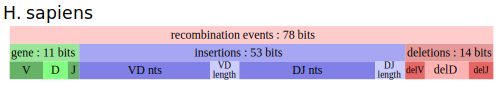
\includegraphics[width = \textwidth]{output_files/figures/pdf/igseq-human-repertoire-entropy}
\Caption{Entropy composition of a human generative repertoire}{Example breakdown of the generative entropy of a human peripheral repertoire, adapted from Figure 8 of Elhanati \textit{et al.} \parencite{elhanati2015model}.} 
\label{fig:igseq-pilot-human-entropies}
\end{figure}

In conclusion, both the generative and realised antibody repertoires of adult male turquoise killifish exhibit substantial sequence diversity, with thousands of detectable clones per individual (\Cref{sec:igseq_pilot_segments}) and billions of unique potential recombination events. While the generative process appears to be highly similar between individuals, the unique life history of the humoral adaptive immune system in each individual provides sufficient information for the secondary repertoires of different individuals to be distinguished based on their V/J-usage profiles (\Cref{sec:igseq_pilot_segments}). Despite its short lifespan, therefore, the turquoise killifish expresses a diverse population of antibody sequences well into middle adulthood, demonstrating its utility as a model organism to investigate the development and ageing of the antibody repertoire.

\FloatBarrier
\clearpage

\section{The effect of ageing on killifish antibody repertoires}
\label{sec:igseq_ageing}

The pilot study into the antibody repertoires of mature adult turquoise killifish (\Cref{sec:igseq_pilot}) demonstrated that these repertoires are diverse and individualised, with a complex generative process giving rise to \naive sequences and an underlying clonal structure resembling that of other species. This pilot dataset, however, consisted of killifish from a single age and treatment group, and therefore gave no information as to the effect of ageing on the composition and diversity of killifish repertoires. In order to investigate the effects of ageing on the killifish antibody repertoire, a second \igseq experiment was performed using all 32 fish described in  \Cref{tab:igseq-cohorts-summary,tab:igseq-cohorts-fish}, comprising 10 fish each sacrificed at 39, 56 and 73 days post-hatching and two fish sacrificed at 128 days post-hatching. Whole-body RNA samples from these fish underwent two independent library preparations as described in \Cref{sec:methods_molec_igseq} and \Cref{sec:igseq_protocol_library}, performed by me and Aleksandra Placzek, for a total of 64 pooled libraries; these were then sequenced together in two MiSeq runs, yielding a total of \embed{output_files/txt/igseq-ageing-nreads-raw-total.txt} million read pairs (\embed{output_files/txt/igseq-ageing-nreads-raw-replicate-min.txt} to \embed{output_files/txt/igseq-ageing-nreads-raw-replicate-max.txt} million pairs per replicate, \embed{output_files/txt/igseq-ageing-nreads-raw-individual-min.txt} to \embed{output_files/txt/igseq-ageing-nreads-raw-individual-max.txt} million pairs per individual), and the resulting reads underwent pre-processing, filtering and clonotyping as described in \Cref{sec:igseq_protocol_preprocess,sec:igseq_pilot_composition,sec:igseq_pilot_clones}.

\Cref{fig:igseq-ageing-read-survival-all} shows the absolute and relative read survival for each of the sixty-four sequencing libraries throughout this process. As with the pilot dataset, the replicates showed relatively consistent behaviour up to and including VDJ assignment and Change-O database construction, with \embed{output_files/txt/igseq-ageing-read-survival-init-min.txt}\,\% to \embed{output_files/txt/igseq-ageing-read-survival-init-max.txt}\,\% of reads surviving up to this stage in the pipeline. However, a somewhat larger number of sequences (\embed{output_files/txt/igseq-ageing-rel-loss-total.txt}\,\% in total, up to \embed{output_files/txt/igseq-ageing-rel-loss-max.txt}\,\% per replicate) were lost during V-score filtering compared to the pilot dataset (\embed{output_files/txt/igseq-pilot-rel-loss-total.txt}\,\% in total, up to \embed{output_files/txt/igseq-pilot-rel-loss-max.txt}\,\% per replicate). This inconsistency was due to a greater preponderance in the ageing dataset of malformed, J-identity-lacking sequences, which in this case actually made up an absolute majority of unique sequences in the \program{pRESTO}-processed dataset (\Cref{fig:igseq-ageing-functional-prop-pre}). After filtering on V-score, however, the functional composition of the ageing dataset was similar to that of the pilot data (\Cref{fig:igseq-ageing-functional-prop-post,fig:igseq-pilot-functional-prop-b}).

\begin{figure}
\centering
\includegraphics[width = 0.9\textwidth]{output_files/figures/pdf/igseq-ageing-read-survival-all}
\begin{subfigure}{0em}
\phantomsubcaption{}
\label{fig:igseq-ageing-read-survival-all-abs}
\end{subfigure}
\begin{subfigure}{0em}
\phantomsubcaption{}
\label{fig:igseq-ageing-read-survival-all-rel}
\end{subfigure}
\Caption{Read survival during pre-processing of the \igseq ageing dataset}{Line graphs of absolute (A) and relative (B) read survival during pre-processing of the \igseq ageing dataset, up to and including clonotyping.}
\label{fig:igseq-ageing-read-survival-all}
\end{figure}

Following V-score filtering, \embed{output_files/txt/igseq-ageing-pc-seq-assigned-clones.txt}\,\% of remaining unique sequences in the ageing dataset were successfully assigned clonal identities. The number of clones inferred per individual ranged from \embed{output_files/txt/igseq-ageing-nclones-individual-min.txt} to \embed{output_files/txt/igseq-ageing-nclones-individual-max.txt}, with a median of \embed{output_files/txt/igseq-ageing-nclones-individual-med.txt}; there was a non-significant (Kruskal-Wallis analysis of variance, $p=\embed{output_files/txt/igseq-ageing-nclones-kruskal-p.txt}$) decline in number of clones per individual with age (\Cref{fig:igseq-ageing-nclones}). These clonal counts were much lower than the median of \embed{output_files/txt/igseq-pilot-nclones-individual-med.txt} clones per individual for the pilot study, reflecting the lower number of reads per individual available in this dataset; for comparison, for the four individuals included in the pilot study, the number of identified clones in the ageing dataset ranged from \embed{output_files/txt/igseq-ageing-nclones-individual-min-pilot.txt} to \embed{output_files/txt/igseq-ageing-nclones-individual-max-pilot.txt}. Concordantly, the distribution of clone sizes detected in the ageing dataset was even more skewed towards small clones than in the pilot dataset: \embed{output_files/txt/igseq-ageing-clones-pc-1count.txt}\,\% of clones were observed as just a single unique sequence across all replicates, while \embed{output_files/txt/igseq-ageing-clones-pc-small.txt}\,\% contained fewer than five unique sequences (\Cref{fig:igseq-ageing-clone-sizes-sizes}). As in the pilot dataset, larger clones were much more likely to be observed across both replicates for a given individual (\Cref{fig:igseq-ageing-clone-sizes-reps}).

\begin{figure}
\centering
\includegraphics[width = 0.8\textwidth]{output_files/figures/pdf/igseq-ageing-clone-diversity}
\Caption{Clonal alpha-diversity spectra for the \igseq ageing dataset}{Bootstrapped alpha-diversity spectra of clone sizes for each age group in the \igseq ageing dataset, as measured by number of unique sequences per clone. Shaded regions in both subfigures represent 95\,\% confidence intervals, estimated using bootstrapping.}
\label{fig:igseq-ageing-clone-diversity-alpha}
\end{figure}

In order to assess the effect of age on the clonal diversity of killifish antibody repertoires, the alpha diversity spectrum of each age group (\Cref{app:diversity-structured-calc}) was computed as described in \Cref{sec:methods_comp_igdownstream_spectra,sec:igseq_pilot_clones}. The resulting spectra, shown in \Cref{fig:igseq-ageing-clone-diversity-alpha}, indicate that repertoire diversity declines monotonically between 5.5 and 10.5 weeks of age in the turquoise killifish, with the most rapid decline observed between 8 and 10.5 weeks: across the entire spectrum, the alpha diversity of the 8-week group is the same as or lower than that of the 5.5 week group, the 10.5-week group is markedly less diverse than the 8-week group, and the 18-week and 10.5-week groups exhibit similar diversity. These observations suggest a model in which repertoire diversity begins declining before or at reproductive maturation (c. 5 weeks post-hatching), declines rapidly in later adulthood, and reaches a plateau of low diversity late in life; however, the smaller size of the 18-week-old group in comparison to the others means that the patterns observed in this group cannot be taken with confidence, and it is possible that a further decline after 10.5 weeks would be observed in a larger sample.

In order to test the significance of these differences in clonal diversity between age groups, the Hill-diversity measurements from each individual spectrum (\Cref{fig:igseq-ageing-clone-diversity-solo-spectra}) were compared across age groups at each of six diversity orders (0, 1, 1.5, 2, 3 and 4) using two distinct methods. In the first, a generalised linear model (GLM) of diversity vs age-at-death was fitted to each diversity order under a gamma distribution, and the resulting model was compared to a null (intercept-only) model to test for a significant ageing effect; in the second, a nonparametric Kruskal-Wallis analysis of variance was used, again to test for a significant effect of age-at-death on the distribution of Hill diversities at a given diversity order. Both results gave roughly consistent results (\Cref{fig:igseq-ageing-clone-diversity-solo-fit-gamma}), as did GLM-based methods assuming a linear or inverse-Gaussian distribution (\Cref{fig:igseq-ageing-clone-diversity-solo-fit-linear,fig:igseq-ageing-clone-diversity-solo-fit-igauss}): in all cases, a significant effect of age on diversity was found for all tested diversity orders above 1.5, but not for order 0 or 1. This pattern, which indicates a significant age effect at higher but not lower diversity orders, suggests that such an effect is driven more by expansion of large clones (which primarily affects higher-order diversity measures) than a decrease in the number of smaller clones (which primarily affects lower-order measures like species richness), a result consistent with the results in \Cref{fig:igseq-ageing-nclones}; if this is the case, it would accord with earlier findings of persistent clonal expansions of activated cells in aged B-cell repertoires in other model systems (\Cref{sec:intro_immunosenescence}).

\begin{figure}
\centering
\includegraphics[width = 0.9\textwidth]{output_files/figures/pdf/igseq-ageing-clone-diversity-solo-fit-gamma}
\Caption{Comparing clonal alpha diversities between age groups in the \igseq ageing dataset}{Boxplots of Hill diversity values for the antibody repertoires of individuals of each age group in the \igseq ageing dataset at a sample of diversity orders, overlaid with the predictions of the best-fit Gamma-distributed generalised linear model at each order.  Annotated $p$-values indicate the statistical significance of the estimated age effect on diversity under the GLM ($P(GLM)$) and a Kruskal-Wallis test ($P(KWT)$) for each diversity order.}
\label{fig:igseq-ageing-clone-diversity-solo-fit-gamma}
\end{figure}

While a significant decline in clonal diversity  was found at various diversity orders, no such decline was observed in the VJ-repertoires of the different age-groups, either when visually comparing the alpha-diversity spectra (\Cref{fig:igseq-ageing-VJ-diversity-alpha}) or statistically comparing the distributions at different diversity orders (\Cref{fig:igseq-ageing-VJ-diversity-solo-fit-gamma,fig:igseq-ageing-vj-diversity-solo-spectra}). This marked difference between the clonal and VJ-repertoires is at first surprising, as a distortion in the clonal repertoire caused by an increased dominance of a few large clones might be expected to cause a similar distortion in the VJ-repertoire by expanding those dominant clones' V/J combinations; however, given that an average of \embed{output_files/txt/igseq-ageing-pc-seq-in-small-clones-avg.txt}\,\% of unique sequences in each repertoire were contained in small clones of fewer than 5 unique sequences (\Cref{fig:igseq-ageing-pc-seq-in-small-clones}), and that this average was not found to change significantly with age (Kruskal-Wallis analysis of variance, $p=\embed{output_files/txt/igseq-ageing-pc-seq-in-small-clones-kruskal-p.txt}$), it may simply be the case that any age-related change in VJ-diversity arising from the minority of sequences sampled from expanded clones was dominated by an absence of change in the V/J-usage distribution of \naive B-cells. To test this hypothesis, I repeated the estimation of VJ-diversity spectra while excluding small clones (containing fewer than five unique sequences); as expected, a clear pattern of reduced alpha diversity with age emerged (\Cref{fig:igseq-ageing-VJ-diversity-large-alpha}), with significant declines in diversity with age observed across all diversity orders tested (\Cref{fig:igseq-ageing-VJ-diversity-large-solo-fit-gamma}).

\begin{figure}
\centering
\includegraphics[width = 0.8\textwidth]{output_files/figures/pdf/igseq-ageing-vj-diversity-all-alpha-beta}
\begin{subfigure}{0em}
\phantomsubcaption{}
\label{fig:igseq-ageing-VJ-diversity-alpha}
\end{subfigure}
\begin{subfigure}{0em}
\phantomsubcaption{}
\label{fig:igseq-ageing-VJ-diversity-beta}
\end{subfigure}
\Caption{VJ-diversity spectra for the \igseq ageing dataset}{Bootstrapped Hill diversity spectra of VJ usage (as measured by number of unique sequences per unambiguous V/J combination) over individuals for each age group in the \igseq ageing dataset. (A) alpha diversity across individuals; (B) beta diversity across individuals, rescaled to between 0 (minimum) and 1 (maximum) in accordance with the number of individuals in each age group. Shaded regions in both subfigures represent 95\,\% confidence intervals, estimated using bootstrapping.}
\label{fig:igseq-ageing-VJ-diversity-spectra}
\end{figure}

\begin{figure}
\centering
\includegraphics[width = 0.8\textwidth]{output_files/figures/pdf/igseq-ageing-vj-diversity-all-solo-fit-gamma}
\Caption{Comparing VJ alpha diversities between age groups in the \igseq ageing dataset}{Boxplots of Hill diversity values for the VJ-repertoires of individuals of each age group in the \igseq ageing dataset at a sample of diversity orders, overlaid with the predictions of the best-fit Gamma-distributed generalised linear model at each order.  Annotated $p$-values indicate the statistical significance of the estimated age effect on diversity under the GLM ($P(GLM)$) and a Kruskal-Wallis test ($P(KWT)$) for each diversity order.}
\label{fig:igseq-ageing-VJ-diversity-solo-fit-gamma}
\end{figure}

\begin{figure}
\centering
\includegraphics[width = 0.8\textwidth]{output_files/figures/pdf/igseq-ageing-vj-diversity-large-alpha-beta}
\begin{subfigure}{0em}
\phantomsubcaption{}
\label{fig:igseq-ageing-VJ-diversity-large-alpha}
\end{subfigure}
\begin{subfigure}{0em}
\phantomsubcaption{}
\label{fig:igseq-ageing-VJ-diversity-large-beta}
\end{subfigure}
\Caption{VJ-diversity spectra for expanded clones in the \igseq ageing dataset}{Bootstrapped Hill diversity spectra of VJ usage (as measured by number of unique sequences per unambiguous V/J combination) over individuals for each age group in the \igseq ageing dataset, excluding clonal groups with fewer than five unique sequences. (A) alpha diversity across individuals; (B) beta diversity across individuals, rescaled to between 0 (minimum) and 1 (maximum) in accordance with the number of individuals in each age group. Shaded regions in both subfigures represent 95\,\% confidence intervals, estimated using bootstrapping.}
\label{fig:igseq-ageing-VJ-diversity-large-spectra}
\end{figure}

\begin{figure}
\centering
\includegraphics[width = 0.8\textwidth]{output_files/figures/pdf/igseq-ageing-vj-diversity-large-solo-fit-gamma}
\Caption{Comparing VJ alpha diversities between age groups for expanded clones in the \igseq ageing dataset}{Boxplots of Hill diversity values for the VJ-repertoires of individuals of each age group in the \igseq ageing dataset at a sample of diversity orders, excluding clonal groups with fewer than five unique sequences, overlaid with the predictions of the best-fit Gamma-distributed generalised linear model at each order.  Annotated $p$-values indicate the statistical significance of the estimated age effect on diversity under the GLM ($P(GLM)$) and a Kruskal-Wallis test ($P(KWT)$) for each diversity order.}
\label{fig:igseq-ageing-VJ-diversity-large-solo-fit-gamma}
\end{figure}

\begin{wraptable}{r}{6.5cm}
\caption{Unique nonfunctional sequences from the \igseq ageing dataset available for model inference with \program{IGoR}}
\label{tab:igseq-ageing-igor-seqs}
% latex table generated in R 3.5.2 by xtable 1.8-3 package
% Fri Mar 15 15:02:31 2019
\begin{tabular}{lr}
  \toprule Age group (days) & \# Unique sequences \\ 
  \midrule 39 & 6107 \\ 
  56 & 5214 \\ 
  73 & 5443 \\ 
  128 & 702 \\ 
   \bottomrule \end{tabular}

\end{wraptable}

The finding that a significant age-related change in VJ-alpha diversity is only observed when small clones are excluded suggests that, while a the secondary antibody repertoire changes significantly with age in the turquoise killifish, the primary generative process does not, at least as far as its statistical composition is concerned. To test this, I inferred generative models for each age group with \program{IGoR} in the manner described in \Cref{sec:igseq_pilot_generative}. Following consensus-sequence inference across clones and discarding of functional sequences, the number of sequences available per individual for this purpose ranged from \embed{output_files/txt/igseq-ageing-igor-seqs-min.txt} to \embed{output_files/txt/igseq-ageing-igor-seqs-max.txt}; all far too low to infer a reliable model with \program{IGoR}. However, pooling these repertoires by age group yielded over 5000 unique sequences for the first three age groups, though the oldest, smallest group yielded only c. 700 sequences total (\Cref{tab:igseq-ageing-igor-seqs}). I therefore investigated the entropy composition of the generative repertoire for the first three age groups in the dataset (\Cref{fig:igseq-ageing-igor-entropies}). The results supported the hypothesis that the generative process remains intact throughout the killifish lifespan, with very similar entropy compositions for all three age groups; neither the total entropy nor any of the major components differs by as much as 1 bit between any two of the three models. Consistent with this, the segment-choice, insertion, and deletion distributions inferred for the generative process are highly similar across all individuals and age groups, despite the very small size of many of the datasets used to infer these models (\Cref{fig:igseq-ageing-igor-segments,fig:igseq-ageing-igor-indels}).

\begin{figure}
\centering
\includegraphics[width = \textwidth]{output_files/figures/pdf/igseq-ageing-igor-entropies}
\Caption{Entropy composition of the killifish generative repertoire in different age groups}{Entropy composition of different diversification mechanisms in the generative process of the turquoise-killifish antibody repertoire, inferred using \program{IGoR} for the first three age groups in the \igseq ageing dataset. ``VD len'' and ``DJ len'' denote sequence variability arising from the number of N-insertions, while ``VD nts'' and ``DJ nts'' refer to variability in the nucleotide sequences so inserted; ``delV'', ``delD'' and ``delJ'' refer to variability arising from deleted (or P-inserted) nucleotides at the boundaries of the selected gene segments. The fourth age group in the dataset (128 days) contained too few nonfunctional sequences to fit a reliable model (\Cref{tab:igseq-ageing-igor-seqs}) and was excluded from the analysis.}
\label{fig:igseq-ageing-igor-entropies}
\end{figure}

While the alpha diversity of the entire VJ-repertoire (reflecting average diversity within each individual repertoire) was not found to change significantly with age in the turquoise killifish, the beta diversity (reflecting inter-individual variability in VJ-expression) showed dramatic differences between age groups, especially at higher diversity orders, for both the entire repertoire (\Cref{fig:igseq-ageing-VJ-diversity-beta}), and the subset of the repertoire contained in large clones (\Cref{fig:igseq-ageing-VJ-diversity-large-beta}): in both cases, while the diversity of the 5.5-week-old group was close to the theoretical minimum for that sample size, the 10.5-week-old group exhibited a substantial increase in inter-individual variability across a wide range of diversity orders, and the 18-week old group showed an even more dramatic increase. This increase in inter-individual diversity with age is corroborated by inter-individual RDI distances computed on VJ-repertoires within each age group: both the overall distribution of inter-individual distances (\Cref{fig:igseq-ageing-rdi-VJ-individual-groupdist-all}), and the distribution of nearest-neighbour distances within each age group (\Cref{fig:igseq-ageing-rdi-VJ-individual-groupdist-nn}), increased significantly with age. This tendency for individuals from increasing age groups to become more distinct in their VJ-repertoires can also be observed using principal co-ordinate analysis:  in \Cref{fig:igseq-ageing-rdi-VJ-individual-pcoa-facet}, the great majority of individuals from younger age groups are visibly more tightly clustered than those from older age groups, which drift apart progressively as age-at-death increases. As in ageing humans (\Cref{sec:intro_immunosenescence}), therefore, the ageing killifish appears to become more individualised and distinct in its antibody repertoire, presumably as the result of an accumulating history of unique individual responses to antigen exposure.

\begin{figure}
\centering
\includegraphics[width = 0.9\textwidth]{output_files/figures/pdf/igseq-ageing-rdi}
\begin{subfigure}{0em}
\phantomsubcaption{}
\label{fig:igseq-ageing-rdi-VJ-individual-groupdist-all}
\end{subfigure}
\begin{subfigure}{0em}
\phantomsubcaption{}
\label{fig:igseq-ageing-rdi-VJ-individual-groupdist-nn}
\end{subfigure}
\begin{subfigure}{0em}
\phantomsubcaption{}
\label{fig:igseq-ageing-rdi-VJ-individual-pcoa-all}
\end{subfigure}
\begin{subfigure}{0em}
\phantomsubcaption{}
\label{fig:igseq-ageing-rdi-VJ-individual-pcoa-facet}
\end{subfigure}
\Caption{Inter-individual VJ-RDI distances in the \igseq ageing dataset}{ (A-B) Boxplots of overall (A) and nearest-neighbour (B) inter-individual VJ-RDI distances for each age group in the \igseq ageing dataset. Pairwise $p$-values were computed using nonparametric Mann-Whitney $U$ tests ($*: 0.01 < p \leq 0.05;~**: 0.001 < p \leq 0.01;~***: p \leq 0.001$). $P(KWT)$ indicates the $p$-value of a Kruskal-Wallis analysis of variance test for a difference in RDI distribution with age. (C-D) Principal co-ordinate analysis (PCoA) of pairwise inter-individual VJ-RDI distances in the \igseq ageing dataset, coloured by age group and displayed together (C) or separately by age group (D).}
\label{fig:igseq-ageing-rdi-VJ-individual}
\end{figure}


\FloatBarrier
\clearpage

\section{Gut-microbiota transfer and the killifish mucosal repertoire}
\label{sec:igseq_gut}

The results from \Cref{sec:igseq_ageing} demonstrate that the whole-body antibody repertoire of adult male turquoise killifish declines in clonal alpha diversity with age, while increasing in VJ beta diversity, with no change observed in the generative process underlying the primary repertoire. These results demonstrate that the turquoise killifish antibody repertoire undergoes rapid age-related changes, in keeping with the more general rapid ageing phenotype observed in this species (\Cref{sec:intro_killifish}). However, while these results demonstrate significant age-related changes in repertoire composition at the level of the entire body, they give no specific information about the ageing process exhibited by the specialised repertoires of particular immune organs, which could differ substantially as a result of their distinct antigenic environments and B-cell-subpopulation composition (\Cref{sec:intro_immunosenescence}). In particular, the gut mucosal repertoire, which polices the interface between the host organism and the gut microbiota, represents a highly important B-cell subpopulation with an intense and distinctive experience of antigenic exposure \parencite{spencer2016intestinal}. It would therefore be interesting to investigate whether the pattern of repertoire ageing observed in the gut accords with that seen in the wider body, or exhibits its own distinct ageing phenotypes.

Smith \textit{et al.} \parencite{smith2017microbiota} demonstrated that gut microbiota transfer from young to middle-aged turquoise killifish significantly extends lifespan in this species, as well as significantly altering microbiotal composition and gene expression in the gut. As part of these experiments, total RNA was isolated from the intestines of a number of male turquoise killifish of the GRZ-Bellemans substrain (a closely-related substrain to the GRZ-AD substrain used in \Cref{sec:igseq_pilot,sec:igseq_ageing}) at different ages and following different experimental interventions (\Cref{fig:igseq-gut-design} and \Cref{tab:gut-cohorts-summary,tab:gut-cohorts-fish}). By using these RNA samples to perform \Igseq, I was able to investigate the effects of both age and microbiota transfer on the diversity of the gut mucosal repertoire; in particular, given the observed lifespan effect of gut-microbiota transfer and the intimate relationship between the gut microbiota and the mucosal adaptive immune system, I hypothesised that gut-microbiota transfer might significantly ameliorate the ageing of the adaptive-immune repertoire observed in \Cref{sec:igseq_ageing}, either through delaying the decline in diversity observed in older fish or by stimulating a renewal of repertoire diversity in mucosal B-cells.

\begin{figure}
\centering
\includegraphics[width = 0.8\textwidth]{output_files/figures/pdf/igseq-gut-design}
\Caption{Experimental design of the killifish gut-microbiota transfer study}{Schematic of the design of the gut-microbiota transfer experiment in Smith \textit{et al.} \parencite{smith2017microbiota}. Groups YI\_6 and WT\_16 were sacrificed without experimental intervention at 6 and 16 weeks, respectively, while the others recieved antibiotic treatment at 9.5 weeks followed by either no further intervention (ABX\_16) or gut-microbiota transfer from a 6-week-old (YMT\_16) or 9.5-week-old (SMT\_16) donor. Adapted from \parencite{smith2017microbiota}, Figure 4.}
\label{fig:igseq-gut-design}
\end{figure}

\begin{table}[b]
\centering
\caption[Summary of killifish used in \igseq gut experiment]{Summary of killifish used in \igseq gut experiment. All fish are GRZ-Bellemans strain and male.}
\label{tab:gut-cohorts-summary}
\input{output_files/tables/igseq-gut-cohorts-summary}
\end{table}

Of the twenty samples outlined in \Cref{tab:gut-cohorts-summary,tab:gut-cohorts-fish}, one (fish 400, from the WT\_16wk group) contained too little RNA to undergo \igseq library preparation, while another (fish 1005, from the OMT\_16wk group) was too degraded for a useful library to be obtained. The remaining 18 samples underwent \igseq library preparation, performed by Aleksandra Placzek and Michael Poeschla using the protocol I designed in \Cref{sec:igseq_protocol_library}. Several of the other samples were also somewhat degraded, with RNA integrity numbers between 5.5 and 7.0 (\Cref{tab:gut-cohorts-fish}), but succeeded in producing useable libraries; these samples were included in the sequencing pool, but the RNA integrity numbers (RIN values) from each sample were retained for comparison with downstream quality-control measures following \Igseq. The resulting libraries were sequenced together in two MiSeq runs, yielding a total of \embed{output_files/txt/igseq-gut-nreads-raw-total.txt} million read pairs (\embed{output_files/txt/igseq-gut-nreads-raw-min.txt} to \embed{output_files/txt/igseq-gut-nreads-raw-max.txt} million pairs per individual), and the resulting reads underwent pre-processing, filtering and clonotyping as described in \Cref{sec:igseq_pilot,sec:igseq_ageing}.

Compared to the datasets in those sections, the gut dataset exhibited highly consistent behaviour up to and including VDJ assignment and Change-O database construction, with \embed{output_files/txt/igseq-gut-read-survival-init-min.txt}\,\% to \embed{output_files/txt/igseq-gut-read-survival-init-max.txt}\,\% of reads surviving up to this stage in the pipeline (\Cref{fig:igseq-gut-read-survival-all}). However, a substantially higher proportion of reads (\embed{output_files/txt/igseq-gut-rel-loss-total.txt}\,\%) were lost during V-score filtering (\Cref{fig:igseq-gut-functional-prop}) and clonotyping, with some individuals losing as much as \embed{output_files/txt/igseq-gut-rel-loss-max.txt}\,\% of their input reads during these stages. The proportion of reads lost at this stage did not appear to have any relationship with the RNA integrity of the samples (\Cref{fig:igseq-gut-read-survival-all-rin}, $r \approx -0.1$, $p \approx 0.7$), and following V-score filtering the functional composition of surviving sequences was similar to that of the other datasets (\Cref{fig:igseq-gut-functional-prop-post,fig:igseq-ageing-functional-prop-post,fig:igseq-pilot-functional-prop-b}). Nevertheless, to avoid any problems associated with very low numbers (and possibly low quality) of surviving input reads, individuals with fewer than 30\,\% of input reads surviving through filtering and clonotyping were excluded from downstream analysis; two individuals (1274 and 1309, both from the ABX\_16 antibiotics-treated group) were excluded in this way (\Cref{fig:igseq-gut-read-survival-all-rel}).

\begin{figure}
\centering
\includegraphics[width = 0.9\textwidth]{output_files/figures/pdf/igseq-gut-read-survival-all}
\begin{subfigure}{0em}
\phantomsubcaption{}
\label{fig:igseq-gut-read-survival-all-abs}
\end{subfigure}
\begin{subfigure}{0em}
\phantomsubcaption{}
\label{fig:igseq-gut-read-survival-all-rel}
\end{subfigure}
\Caption{Read survival during pre-processing of the \igseq gut dataset}{Line graphs of absolute (A) and relative (B) read survival during pre-processing of the \igseq gut dataset, up to and including clonotyping. The dotted red line in (B) indicates the 30\,\% read-survival cutoff, below which samples were discarded prior to downstream analysis.}
\label{fig:igseq-gut-read-survival-all}
\end{figure}

Following V-score filtering and exclusion of high-read-loss individeals, \embed{output_files/txt/igseq-gut-pc-seq-assigned-clones.txt}\,\% of remaining unique sequences in the ageing dataset were successfully assigned clonal identities, with the number of clones inferred per individual ranging from \embed{output_files/txt/igseq-gut-nclones-individual-min.txt} to \embed{output_files/txt/igseq-gut-nclones-individual-max.txt}, with a median of \embed{output_files/txt/igseq-gut-nclones-individual-med.txt}; as in the ageing dataset, there was a non-significant (Kruskal-Wallis analysis of variance, $p=\embed{output_files/txt/igseq-gut-nclones-kruskal-age-p.txt}$) decline in number of clones per individual with age (\Cref{fig:igseq-gut-nclones}). With two exceptions (visible as outliers in \Cref{fig:igseq-gut-nclones}), these clonal counts are dramatically lower than those of either the pilot or ageing dataset, both in absolute terms (\Cref{fig:igseq-comparative-metrics-abs}) and relative to the number of UMI groups or unique sequences in each repertoire (\Cref{fig:igseq-comparative-metrics-rel}). This suggests, not entirely surprisingly, that killifish guts contain many fewer B-cell clones than whole-body killifish samples. However, the metrics presented in \Cref{fig:igseq-comparative-metrics} are strongly dependent on the size of each dataset and cannot be taken at face value: for example, even though the pilot dataset contains the same type of sample and even a subset of the same individuals from the ageing dataset, their distributions in \Cref{fig:igseq-comparative-metrics} are very different.

\begin{figure}
\centering
\includegraphics[width = 0.8\textwidth]{output_files/figures/pdf/igseq-gut-nclones}
\Caption{Number of clones in the \igseq gut dataset}{Boxplots of clonal counts for each individual in the \igseq gut dataset, grouped by age at death (A) or treatment group (B). The apparent decline in clonal count with age is not significant (Kruskal-Wallis analysis of variance, $p=\embed{output_files/txt/igseq-gut-nclones-kruskal-age-p.txt}$), and there is also no significant effect of treatment group on clonal count (Kruskal-Wallis analysis of variance, $p=\embed{output_files/txt/igseq-gut-nclones-kruskal-group-p.txt}$).}
\label{fig:igseq-gut-nclones}
\end{figure}

\begin{figure}
\centering
\includegraphics[width = 0.9\textwidth]{output_files/figures/pdf/igseq-nclones-comparative}
\begin{subfigure}{0em}
\phantomsubcaption{}
\label{fig:igseq-comparative-metrics-abs}
\end{subfigure}
\begin{subfigure}{0em}
\phantomsubcaption{}
\label{fig:igseq-comparative-metrics-rel}
\end{subfigure}
\Caption{Comparison of clonal counts between \igseq experiments}{Boxplots comparing different count metrics between the \igseq pilot, ageing and gut datasets, demonstrating the reduced absolute and relative clonal counts in the latter. (A) Absolute numbers of UMI groups, unique sequences and clones in each dataset. (B) Relative numbers of UMI groups and unique sequences per clone.}
\label{fig:igseq-comparative-metrics}
\end{figure}

In order to determine whether the apparent difference in clonal richness between the gut and other datasets is real, therefore, I performed rarefaction analysis, measuring the number of clones and P20 in repeated downsamplings of UMI groups from each dataset. The results for the rarefied clonal counts (\Cref{fig:igseq-rarefied-clone-counts}) confirmed the results from \Cref{fig:igseq-comparative-metrics}: at any given downsampling size, the great majority of repertoires from the gut dataset contained far fewer clones than the repertoires in the pilot or ageing datasets. The gut repertoires also showed a much greater degree of dominance by the largest clones in each repertoire (\Cref{fig:igseq-rarefied-clone-p20}), with over 85\,\% of gut samples exhibiting greater asymptotic P20 than over 90\,\% of ageing or pilot individuals and over 65\,\% exhibiting higher asymptotic P20 than any sample in either of the other experiments. In both cases (clonal counts and P20), a small minority of individuals deviated strongly from the general trend, exhibiting clonal counts and P20 values more consistent with those seen in the pilot and ageing experiments; however, only one individual (1412, from the YI\_6 6-week-old untreated group) was an outlier in both clonal count and P20 value.

\begin{figure}
\centering
\includegraphics[width = 0.9\textwidth]{output_files/figures/pdf/igseq-rarefied-clones}
\begin{subfigure}{0em}
\phantomsubcaption{}
\label{fig:igseq-rarefied-clone-counts}
\end{subfigure}
\begin{subfigure}{0em}
\phantomsubcaption{}
\label{fig:igseq-rarefied-clone-p20}
\end{subfigure}
\Caption{Comparative rarefaction analysis of clonal counts and P20 in \igseq experiments}{Rarefaction analysis of (A) clonal counts and (B) P20 in turquoise killifish repertoires from the \igseq pilot, ageing and gut-microbiota-transfer experiments. Lines and shaded regions indicate the mean and standard deviation, respectively, over twenty replicates per sample size.}
\label{fig:igseq-rarefied-clones}
\end{figure}

The combination of low clonal counts and elevated P20 indicated by \Cref{fig:igseq-rarefied-clone-counts,fig:igseq-rarefied-clone-p20} suggests that the intestinal antibody repertoire of the turquoise killifish contains many fewer small, \naive clones than the whole-body repertoire, and is consequently much more strongly dominated by a comparatively small number of expanded clones. This hypothesis is confirmed when the rarefied clonal counts are separated by clone size (\Cref{fig:igseq-rarefied-clone-counts-size}): while the number of small clones (containing fewer than 5 unique sequences) in the gut repertoires was again much smaller than in the other experiments (\Cref{fig:igseq-rarefied-clone-counts-small}), the number of large clones (containing at least 5 unique sequences) was roughly the same (\Cref{fig:igseq-rarefied-clone-counts-large}), and as a consequence the proportion of large clones was much higher in most gut repertoires than in the whole body (\Cref{fig:igseq-rarefied-clone-counts-large-pc}). This difference between the gut and whole-body repertoires makes sense: unlike the gut repertoire, the whole-body repertoire includes clones from primary lymphoid organs (in particular, the anterior kidney), and so could be expected to contain a much larger number of small, \naive clones. Furthermore, as a site of extensive interaction between the host and the gut microbiota, the gut provides many opportunities for its resident B-cells to encounter foreign antigens \parencite{caruso2009immunosenescence}, and the consequent high rate of clonal expansion is likely to further increase the extent to which the gut repertoire is dominated by large clones.

\begin{figure}
\centering
\includegraphics[width = \textwidth]{output_files/figures/pdf/igseq-rarefied-clone-counts-size}
\begin{subfigure}{0em}
\phantomsubcaption{}
\label{fig:igseq-rarefied-clone-counts-small}
\end{subfigure}
\begin{subfigure}{0em}
\phantomsubcaption{}
\label{fig:igseq-rarefied-clone-counts-large}
\end{subfigure}
\begin{subfigure}{0em}
\phantomsubcaption{}
\label{fig:igseq-rarefied-clone-counts-large-pc}
\end{subfigure}
\Caption{Comparative rarefaction analysis of clonal size composition in \igseq experiments}{Rarefaction curves of (A) the number of small clones ($<5$ unique sequences), (B) the number of large clones ($\geq 5$ unique sequences) and (C) the proportion of clones which are large in each individual, coloured by source experiment. Lines and shaded regions indicate the mean and standard deviation, respectively, over twenty replicates per sample size.}
\label{fig:igseq-rarefied-clone-counts-size}
\end{figure}

The clonal alpha-diversity spectra for the gut dataset are shown in \Cref{fig:igseq-gut-clone-diversity-alpha}. At all diversity orders, there is a clear and drastic difference between the young (6-week-old) and old (16-week-old) groups, while the different 16-week-old treatment groups do not appear to show a strong difference in diversity. These observations are confirmed by statistical comparison of the distributions of individual diversity measurements at different diversity orders, which indicate highly significant differences in clonal repertoire diversity between young and old guts across the diversity spectrum (\Cref{fig:igseq-gut-clone-diversity-solo-age,fig:igseq-gut-clone-diversity-solo-spectra-age}), but no difference between treatment groups (\Cref{fig:igseq-gut-clone-diversity-solo-groups,fig:igseq-gut-clone-diversity-solo-spectra-groups}). A similar pattern is observed for V/J-usage diversity (\Cref{fig:igseq-gut-VJ-diversity-alpha}), with a large and significant difference between young and old cohorts at many different diversity orders (\Cref{fig:igseq-gut-VJ-diversity-solo-age,fig:igseq-gut-vj-diversity-solo-spectra-age}) but no significant differences between 16-week-old treatment groups (\Cref{fig:igseq-gut-VJ-diversity-solo-groups,fig:igseq-gut-vj-diversity-solo-spectra-groups}).

\begin{figure}
\centering
\includegraphics[width = 0.9\textwidth]{output_files/figures/pdf/igseq-gut-clone-diversity-alpha}
\begin{subfigure}{0em}
\phantomsubcaption{}
\label{fig:igseq-gut-clone-diversity-alpha-age}
\end{subfigure}
\begin{subfigure}{0em}
\phantomsubcaption{}
\label{fig:igseq-gut-clone-diversity-alpha-groups}
\end{subfigure}
\Caption{Clonal alpha-diversity spectra for the \igseq gut dataset}{Bootstrapped alpha-diversity spectra of clone sizes for each (A) age group and (B) treatment group in the \igseq gut dataset, as measured by number of unique sequences per clone. Shaded regions in both subfigures represent 95\,\% confidence intervals, estimated using bootstrapping.}
\label{fig:igseq-gut-clone-diversity-alpha}
\end{figure}

\begin{figure}
\centering
\begin{subfigure}{0em}
\phantomsubcaption{}
\label{fig:igseq-gut-clone-diversity-solo-age}
\end{subfigure}
\begin{subfigure}{0em}
\phantomsubcaption{}
\label{fig:igseq-gut-clone-diversity-solo-groups}
\end{subfigure}
\includegraphics[width = 0.9\textwidth]{output_files/figures/pdf/igseq-gut-clone-diversity-solo-boxplots}
\Caption{Comparing clonal alpha diversities between age and treatment groups in the \igseq gut dataset}{Boxplots of clonal Hill diversity values for the antibody repertoires of individuals of each (A) age group and (B) treatment group in the \igseq gut dataset at a sample of diversity orders. Pairwise $p$-values were computed using nonparametric Mann-Whitney $U$ tests ($*: 0.01 < p \leq 0.05;~**: 0.001 < p \leq 0.01;~***: p \leq 0.001$).}
\label{fig:igseq-gut-clone-diversity-solo-boxplots}
\end{figure}

\begin{figure}
\centering
\includegraphics[width = 0.9\textwidth]{output_files/figures/pdf/igseq-gut-vj-diversity-alpha}
\begin{subfigure}{0em}
\phantomsubcaption{}
\label{fig:igseq-gut-VJ-diversity-alpha-age}
\end{subfigure}
\begin{subfigure}{0em}
\phantomsubcaption{}
\label{fig:igseq-gut-VJ-diversity-alpha-groups}
\end{subfigure}
\Caption{VJ alpha-diversity spectra for the \igseq gut dataset}{Bootstrapped alpha-diversity spectra of VJ usage for each (A) age group and (B) treatment group in the \igseq gut dataset, as measured by number of unique sequences per unambiguous VJ identity. Shaded regions in both subfigures represent 95\,\% confidence intervals, estimated using bootstrapping.}
\label{fig:igseq-gut-VJ-diversity-alpha}
\end{figure}

\begin{figure}
\centering
\begin{subfigure}{0em}
\phantomsubcaption{}
\label{fig:igseq-gut-VJ-diversity-solo-age}
\end{subfigure}
\begin{subfigure}{0em}
\phantomsubcaption{}
\label{fig:igseq-gut-VJ-diversity-solo-groups}
\end{subfigure}
\includegraphics[width = 0.9\textwidth]{output_files/figures/pdf/igseq-gut-vj-diversity-solo-boxplots}
\Caption{Comparing VJ alpha diversities between age and treatment groups in the \igseq gut dataset}{Boxplots of VJ Hill diversity values for the antibody repertoires of individuals of each (A) age group and (B) treatment group in the \igseq gut dataset at a sample of diversity orders. Pairwise $p$-values were computed using nonparametric Mann-Whitney $U$ tests ($*: 0.01 < p \leq 0.05;~**: 0.001 < p \leq 0.01;~***: p \leq 0.001$).}
\label{fig:igseq-gut-VJ-diversity-solo-boxplots}
\end{figure}

In terms of beta diversity, the Hill-spectrum results (\Cref{fig:igseq-gut-VJ-diversity-beta}) are equivocal, with large differences in diversity between age groups observed at intermediate diversity orders (c. 1 to 2.5) but not at very low or very high orders (\Cref{fig:igseq-gut-VJ-diversity-beta-age}). Different treatment groups, meanwhile, exhibit very different patterns of beta diversity at higher orders (\Cref{fig:igseq-gut-VJ-diversity-beta-groups}), but not in any clear pattern: the antibiotic-treated and same-age-transfer groups show near-maximal high-order beta diversity, indicating dramatic differences between individuals in their VJ-usage profiles, while the untreated and young-donor-transfer groups show much lower between-individual variablity. To more closely investigate differences in inter-individual variability between sample groups, I again computed repertoire dissimilarity index (RDI) distances between each pair of individual repertoires in the dataset, and visualised the results by age cohort (\Cref{fig:igseq-gut-rdi-VJ-individual-age}) and treatment group (\Cref{fig:igseq-gut-rdi-VJ-individual-group}). As in the ageing dataset, these results indicate large differences in VJ-usage variability between young and old intestinal repertoires in the turquoise killifish, with young samples clustering much more closely together (\Cref{fig:igseq-gut-rdi-VJ-individual-age-pcoa-facet}) and consequently exhibiting much lower pairwise RDI distances (\Cref{fig:igseq-gut-rdi-VJ-individual-age-groupdist-all,fig:igseq-gut-rdi-VJ-individual-age-groupdist-nn}); conversely, there is no significant difference in RDI distribution between the different 16-week-old treatment groups (\Cref{fig:igseq-gut-rdi-VJ-individual-group-groupdist-all,fig:igseq-gut-rdi-VJ-individual-group-groupdist-nn}), indicating that the different groups are similar in their inter-individual variability. These RDI results contrast markedly with the differences in beta-diversity spectra observed in \Cref{fig:igseq-gut-VJ-diversity-beta-groups}, suggesting that the latter may not be reliable measures of significant differences in intra-group variablity when sample sizes are small.

\begin{figure}
\centering
\includegraphics[width = 0.9\textwidth]{_output_files/figures/pdf/igseq-gut-vj-diversity-beta}
\begin{subfigure}{0em}
\phantomsubcaption{}
\label{fig:igseq-gut-VJ-diversity-beta-age}
\end{subfigure}
\begin{subfigure}{0em}
\phantomsubcaption{}
\label{fig:igseq-gut-VJ-diversity-beta-groups}
\end{subfigure}
\Caption{VJ beta-diversity spectra for the \igseq gut dataset}{Bootstrapped beta-diversity spectra of VJ usage for each (A) age group and (B) treatment group in the \igseq gut dataset, as measured by number of unique sequences per unambiguous VJ identity, rescaled to between 0 (minimum) and 1 (maximum) for each individual. Shaded regions in both subfigures represent 95\,\% confidence intervals, estimated using bootstrapping.}
\label{fig:igseq-gut-VJ-diversity-beta}
\end{figure}

\begin{figure}
\centering
\includegraphics[width = 0.9\textwidth]{output_files/figures/pdf/igseq-gut-rdi-age}
\begin{subfigure}{0em}
\phantomsubcaption{}
\label{fig:igseq-gut-rdi-VJ-individual-age-pcoa-all}
\end{subfigure}
\begin{subfigure}{0em}
\phantomsubcaption{}
\label{fig:igseq-gut-rdi-VJ-individual-age-pcoa-facet}
\end{subfigure}
\begin{subfigure}{0em}
\phantomsubcaption{}
\label{fig:igseq-gut-rdi-VJ-individual-age-groupdist-all}
\end{subfigure}
\begin{subfigure}{0em}
\phantomsubcaption{}
\label{fig:igseq-gut-rdi-VJ-individual-age-groupdist-nn}
\end{subfigure}
\Caption{Intra-age-group variability in VJ expression in the \igseq gut dataset}{(A-B) Principal co-ordinate analysis (PCoA) of pairwise inter-individual VJ-RDI distances in the \igseq gut dataset, coloured by age group and displayed together (A) or separately by age group (B). (C-D) Boxplots of overall (C) and nearest-neighbour (D) inter-individual VJ-RDI distances for each age group in the dataset. Pairwise $p$-values were computed using nonparametric Mann-Whitney $U$ tests ($*: 0.01 < p \leq 0.05;~**: 0.001 < p \leq 0.01;~***: p \leq 0.001$).}
\label{fig:igseq-gut-rdi-VJ-individual-age}
\end{figure}

\begin{figure}
\centering
\includegraphics[width = 0.9\textwidth]{output_files/figures/pdf/igseq-gut-rdi-group}
\begin{subfigure}{0em}
\phantomsubcaption{}
\label{fig:igseq-gut-rdi-VJ-individual-group-pcoa-all}
\end{subfigure}
\begin{subfigure}{0em}
\phantomsubcaption{}
\label{fig:igseq-gut-rdi-VJ-individual-group-pcoa-facet}
\end{subfigure}
\begin{subfigure}{0em}
\phantomsubcaption{}
\label{fig:igseq-gut-rdi-VJ-individual-group-groupdist-all}
\end{subfigure}
\begin{subfigure}{0em}
\phantomsubcaption{}
\label{fig:igseq-gut-rdi-VJ-individual-group-groupdist-nn}
\end{subfigure}
\Caption{Intra-treatment-group variability in VJ expression in the \igseq gut dataset}{(A-B) Principal co-ordinate analysis (PCoA) of pairwise inter-individual VJ-RDI distances in the \igseq gut dataset, coloured by treatment group and displayed together (A) or separately by treatment group (B). (C-D) Boxplots of overall (C) and nearest-neighbour (D) inter-individual VJ-RDI distances for each treatment group in the dataset. Pairwise $p$-values were computed using nonparametric Mann-Whitney $U$ tests ($*: 0.01 < p \leq 0.05;~**: 0.001 < p \leq 0.01;~***: p \leq 0.001$).}
\label{fig:igseq-gut-rdi-VJ-individual-group}
\end{figure}

In terms of repertoire ageing, therefore, the killifish intestinal repertoire not only reproduces the whole-body phenotype of reduced alpha and increased beta diversity with age, but in fact shows a stronger ageing phenotype than the whole-body repertoires reported in \Cref{sec:igseq_ageing}. In addition to showing a much stronger age-related decline in clonal alpha diversity with age than that exhibited in the ageing dataset (\Cref{fig:igseq-ageing-clone-diversity-alpha,fig:igseq-ageing-clone-diversity-solo-fit-gamma,fig:igseq-gut-clone-diversity-alpha-age,fig:igseq-gut-clone-diversity-solo-age}), the gut repertoire also shows a significant age-related decline in VJ alpha diversity, something not observed in the whole-body data (\Cref{fig:igseq-ageing-VJ-diversity-alpha,fig:igseq-ageing-VJ-diversity-solo-fit-gamma,fig:igseq-gut-VJ-diversity-alpha-age,fig:igseq-gut-VJ-diversity-solo-age}). This latter difference is likely due to the much lower clonal richness and higher oligoclonality exhibited by the gut repertoires (\Cref{fig:igseq-rarefied-clone-counts,fig:igseq-rarefied-clone-p20,fig:igseq-rarefied-clone-counts-size}): when the local repertoire contains fewer small \naive clones and exhibits a greater degree of domination by the few largest clones, differences in VJ-usage between these large, activated clones may outweigh unchanged VJ-usage distributions in small, \naive clones to a greater extent than in the much-more-polyclonal whole-body repertoire. The much more dramatic loss of clonal diversity in intestinal repertoires, meanwhile, may be attributable to the especially-intense antigenic challenge at the mucosal surface, resulting in high levels of clonal expansion and progressive domination of the mucosal B-cell niche by a small number of highly expanded clones \parencite{caruso2009immunosenescence}; this phenomenon could in turn be exacerbated by the observed loss of taxonomic diversity (but not total abundance) in the gut microbiota \parencite{smith2017microbiota}, which might progressively reduce the variety of antigenic exposure at the mucosal surface and so further encourage a restriction in clonal diversity. If so, the strength of the ageing phenotype in these repertoires may have important consequences for the ability of the organism to regulate its mucosal microbial environment. More research is needed, however, to determine the mechanisms, kinetics and importance of mucosal-repertoire ageing in turquoise killifish.

In sharp contrast to the age-related changes observed in the gut antibody repertoire, there is no clear evidence from these analyses supporting the hypothesis that gut-microbiota transfer from young fish rejuvenates the antibody repertoire. While the alpha diversity spectrum of the YMT\_16 group appears to be slightly higher than the SMT\_16/ABX\_16 groups at very low diversity orders (\Cref{fig:igseq-gut-clone-diversity-alpha-groups}), these indications are not borne out by subsequent statistical analysis, and it is precisely these low-order diversity metrics that are most vulnerable to sampling bias and undersampling (\Cref{app:diversity-unitary-hill}), a pervasive problem in immune-repertoire sequencing \parencite{mora2016diversity}. There is also no obvious difference in VJ alpha diversity between treatment groups, while the beta diversity of the YMT\_16 group is non-significantly \textit{higher} than that of the untreated control group (\Cref{fig:igseq-gut-VJ-diversity-beta-groups,fig:igseq-gut-rdi-VJ-individual-group-groupdist-all}). Overall, whatever mechanism underlies the effect of gut microbiota transfer on killifish lifespan \parencite{smith2017microbiota}, it does not appear to be operating through modulation of gut antibody-repertoire diversity.

\FloatBarrier
\clearpage

\section{Discussion}
\label{sec:igseq_discussion}

Apart from the nervous system itself, no other system in the vertebrate body exhibits such complex learning behaviour as the adaptive immune system. Through the combination of an extremely diverse generative repertoire, antigen-dependent clonal expansion, and extremely long-lasting immune memory, the adaptive immune system progressively learns to model its immune environment and predict -- and defend against -- future pathogenic attacks \parencite{mayer2018memory}. During ageing, however, this predictive and protective ability progressively declines through a combination of a loss of adaptivity and overexpansion of previously established memory clones, leaving the body unable to effectively protect itself from novel infections or establish adequate immune memory in response to vaccination or other antigenic challenges (\Cref{sec:intro_immunosenescence}). Learning more about the mechanisms, spatial distribution and temporal progression of this age-related decline in adaptive immunity constitutes an essential part of the study of vertebrate ageing.

In this chapter, I established the first working library-preparation protocol and sequence-analysis pipeline for immunoglobulin sequencing in turquoise killifish (\nfu), a highly promising emerging model for vertebrate ageing and immunosenescence (\Cref{sec:intro_killifish}), and investigated the composition, diversity and ageing of \igh{M} antibody repertoires in adult males of this species. The results demonstrated that killifish express diverse and individualised antibody repertoires, with thousands of clones and billions of potential unique sequences per individual, which are both reproducible between replicates from the same individual and distinguishable between different individuals of the same age and inbred strain (\Cref{sec:igseq_pilot_clones,sec:igseq_pilot_generative}). With the exception of the very largest clones, these repertoires conformed to the heavy-tailed Zipf-like distribution of clone sizes observed in other species, and thus exhibited a clonal structure divided between a very large number of very small clones and a much smaller number of highly expanded clones.

Over the course of adulthood, these larger clones exhibit a progressive loss of diversity due to accumulating clonal expansions, leading to reduced alpha diversity of the clonal repertoire at higher diversity orders (when small clones are strongly downweighted compared to large ones) and a progressive loss in alpha VJ-diversity among large clones (\Cref{sec:igseq_ageing}). At the same time, the most expanded V/J-combinations become progressively more different in older killifish, resulting in an increase in beta diversity which is particularly strong at high diversity orders. This loss of alpha diversity and increase in beta diversity with age in turquoise killifish is in line with observations made previously in human peripheral blood (\Cref{sec:intro_immunosenescence}). Small clones, by contrast, appear to exhibit much less change in repertoire composition with age in whole-body killifish samples: there is a non-significant decline in total clonal count and low-order clonal alpha-diversity in older killifish antibody repertoires, and any significant change in alpha VJ-diversity disappears when small clones are included. In addition, the complexity of the generative process giving rise to novel antibody sequences does not appear to change between age groups, suggesting that newly-produced \naive B-cells may be of similar diversity in young and old killifish.

These results do not necessarily demonstrate that the repertoire composition of small clones in turquoise killifish is unchanged with age; several metrics, including clonal richness, decline non-significantly with age, and it may be the case that significant changes would become apparent with larger sample sizes or a different set of data-generation and -analysis methods. A comprehensive assessment of \naive B-cell repertoires in ageing killifish would require more specialised laboratory techniques (such as cell sorting of B-cell subtypes) and examination of processes such as primary selection that have been neglected in this analysis. One important alternative explanation relates to body size: unlike humans and mice, turquoise killifish grow continuously with age (\Cref{tab:igseq-cohorts-summary,tab:igseq-cohorts-fish}), and it is possible that an age-related decline in the rate of B-cell output by the primary lymphoid organs is offset by a continuous increase in the size of these organs with age. Nevertheless, these results do suggest that the bulk of the change in the \igh{M} repertoire of ageing killifish arises from changes in the size and composition of expanded antigen-experienced clones rather than changes in the \naive compartment. If this is the case, it raises the question of to what extent these changes, including the observed loss in diversity, represent functional declines as a result of ageing, rather than the expected and functional result of progressive immune adaptation to a controlled laboratory environment. Such a question is an important one, but lies outside the scope of the experiments and analyses presented in this chapter.

As discussed above, the inferred entropy of the heavy-chain generative process in turquoise killifish does not appear to change much with age, with estimates varying between 30 and 32 bits (\Cref{sec:igseq_pilot_generative}). Antibody generation in turquoise killifish is therefore a highly complex and diverse process, with the number of potentially-generable sequences exceeding $10^9$, but is nevertheless  vastly less diverse than the equivalent process in humans (which can potentially produce in excess of $10^{21}$ different sequences). A lower potential repertoire diversity in killifish compared to humans is not necessarily surprising, given the much greater size and number of gene segments in the human \igh{} locus; unexpectedly, however, most of the observed difference in diversity does not reflect a general discrepency across all contributing processes, but rather a specific and very large (in excess of 40 bits) difference in the complexity of the N-insertion process alone. This specific difference reflects the very different N-insertion distributions in humans and killifish, with the former showing much larger mean, median and modal numbers of insertions compared to the latter \parencite{elhanati2015model}. The cause of this difference is not known, nor whether it is specific to turquoise killifish or a more general feature of teleost antibody repertoires; however, it seems likely to involve the structure, expression or regulation of the terminal dideoxy transferase enzyme (TdT) responsible for the N-insertion process. At least one orthologue of human TdT is annotated in the turquoise killifish genome, and more detailed investigation of the structure and function of this enzyme in \nfu and related species may reveal unexpected insights into the mechanism and regulation of the N-insertion process during primary antibody diversification.

As early as 2009, Caruso \textit{et al.} \parencite{caruso2009immunosenescence} commented that the mucosal adaptive immune system might exhibit particularly strong loss of diversity with age, as a result of especially frequent antigenic challenge. Nevertheless, to my knowledge, no previous study has specifically investigated antibody-repertoire ageing in a mucosal immune organ such as the gut. In this chapter, I performed the first such analysis, investigating changes in antibody diversity in RNA samples from the guts of young and old killifish (\Cref{sec:igseq_gut}). The results strongly confirmed Caruso \textit{et al.}'s prediction: not only did gut mucosal antibody repertoires exhibit a much greater degree of clonal expansion compared to the whole-body repertoire (as shown by differences in both P20 and the proportion of large clones), but both the clonal and VJ-repertoires exhibited a dramatic drop in diversity with age across all diversity orders, to a much larger extent than observed in whole-body samples; as in the whole-body repertoire, these changes were also accompanied by a large increase in beta VJ-diversity between older individuals. These results demonstrate that the killifish gut exhibits dramatic changes in both clonal structure and VJ-usage with age; given the much greater predominance of expanded clones in the gut repertoire, such differences in ageing phenotypes between the gut and whole-body repertoires further support the conclusion that changes in repertoire composition with age in the killifish are primarily driven by expanded, antigen-experienced clones rather than the \naive compartment. Given these results, it would be interesting to investigate other mucosal immune organs (such as the gills and skin \parencite{xu2013igtskin}) to see if these ageing phenotypes represent a general pattern or are specific to the intestinal mucosa.

In stark contrast to the striking drop in diversity with age in the killifish intestinal repertoire, no change in repertoire diversity was observed as a result of gut microbial transfer from young donor fish. In part, the small size of each treatment group among the old gut samples makes drawing any strong conclusions difficult, but nevertheless there was no indication that the young-donor group showed any delay or reversal in any of the ageing phenotypes observed in the mucosal antibody repertoire. This lack of change in the repertoire is to some extent surprising, as microbiota transfer has been shown to affect gut microbial diversity in older fish, which might be expected to in turn affect the diversity of the antibody repertoire; the lack of effect observed in this chapter suggests that the link between microbial and immune-repertoire diversity is slower, weaker or more indirect than this simple description would suggest, though more research is needed to determine exactly what the connection between the diversities of the two systems might in fact be. 

Despite the apparent lack of effect on intestinal antibody-repertoire diversity resulting from gut microbial transfer, the effect of anti-ageing interventions on age-related changes in the antibody repertoire remains an important and underexplored topic of study. To my knowledge, nothing is known about how well-established pro-longevity interventions like dietary restriction, rapamycin treatment or reduced insulin/IGF1 signaling \parencite{lopezotin2013hallmarks} affect the ageing of the antibody repertoire, whether in the gut, peripheral blood or elsewhere. Given its short lifespan, highly scalable husbandry conditions, and demonstrated age-dependent changes in the antibody repertoire, the turquoise killifish would be an ideal model organism in which to elaborate this intersection between the biology of ageing and vertebrate immunology, with the potential to identify new and important interrelationships between longevity pathways and the adaptive immune system.

As suggested by the foregoing paragraph, the work included in this chapter is only the tip of an iceberg of potential research into adaptive immunosenescence that could be performed with the turquoise killifish. Even using the datasets already generated for this chapter, a great deal of research remains to be done on the state and ageing of antibody repertoires in this species. Particularly important topics left unexplored in this thesis include the rate, distribution and ageing of somatic hypermutation in killifish repertoires; the efficacy of clonal selection during affinity maturation (\Cref{sec:intro_affinity_maturation}); and whether any age-related changes affect the primary-selection process separating the generation of new antibody sequences from the \naive antibody repertoire. Further experiments could substantially improve our understanding of the origins and ageing of killifish antibody repertoires by incorporating light-chain sequence and heavy-chain/light-chain pairing information or by supplementing bulk repertoire-sequencing data with higher-resolution single-cell data from sorted \naive or antigen-experienced B-cells \parencite{friedensohn2017advanced}, while studies involving infection, vaccination or other immune interventions could explore the functional implications of a loss of repertoire diversity with age.

Such experiments, however, would require the development of important additional resources for the turquoise killifish model, including reliable antibodies and cell-surface markers, characterisation of the light-chain gene loci, and optimised single-cell repertoire-sequencing techniques, work that is still ongoing in several killifish labs worldwide. Simpler but still-valuable experiments could investigate a greater range of timepoints and immune organs, incorporate data from \igh{D} or separate secretory and transmembrane \igh{M} repertoires, or extend our knowledge of killifish antibody repertoires to development and early adulthood. Eventually, a whole-body, whole-lifespan atlas of adaptive-immune ageing in the killifish could reveal a great deal of information about how and why the antibody repertoires of ageing vertebrates exhibit the compositional and functional changes they do, with important consequences for biogerontological research, comparative immunology, and drug development.
\include{input_files/tex/C5_Conclusion}

% ********************************** Bibliography ******************************

\begin{spacing}{0.9}
\printbibliography[heading=bibintoc, title={References}]
\end{spacing}

% ********************************** Appendices ********************************

\begin{appendices} % Using appendices environment for more functionality
\appendix
\include{input_files/tex/D1_Solutions}
\include{input_files/tex/D2_Primers}
\include{input_files/tex/D3_Diversity}
\chapter{Supplementary figures}
\label{app:figures}

% 3 - LOCUS CHAPTER

\begin{figure}
	\centering
	\includegraphics[width=0.9\textwidth]{output_files/figures/pdf/locus-nfu-rss-seqlogo-sep}
	\Caption{\Nfu recombination signal sequences by segment type}{Sequence composition of conserved heptamer (A,C,E) and nonamer (B,D,F) sequences from \Nfu heavy-chain RSSs associated with \vh (A,B), \dh (C,D) or \jh (E,F) gene segments.}
	\label{fig:nfu-rss-seqlogo-sep}
\end{figure}

	\begin{figure}
	\centering
	\includegraphics[width=\textwidth]{output_files/figures/pdf/locus-xma-vh-families-map}
	\Caption{Heatmap of \vh families in the \Xma \igh{} locus}{Heatmap of family relationships among \Xma \vh segments, with coloured shading indicating families and red dots indicating pairwise nucleotide sequence identity of at least 80\%. \vh families containing multiple segments are uniquely coloured, while single-segment families are in grey.}
	\label{fig:xma-vh-families-map}
	\end{figure}

	\begin{figure}
	\centering
	\includegraphics[width=0.9\textwidth]{output_files/figures/pdf/locus-xma-rss-seqlogo-sep}
	\Caption{\Xma recombination signal sequences by segment type}{Sequence composition of conserved heptamer (A,C,E) and nonamer (B,D,F) sequences from \Xma heavy-chain RSSs associated with \vh (A,B), \dh (C,D) or \jh (E,F) gene segments.}
	\label{fig:xma-rss-seqlogo-sep}
	\end{figure}
	
	\begin{figure}
\centering
\includegraphics[width=0.9\textwidth]{output_files/figures/pdf/locus-comp-ch-tree}
\Caption{Constant-region \ch exons in the Atherinomorpha}{Unrooted phylogram of \ch exons from thirteen fish species from the Atherinomorpha (\Cref{tab:cyprinodontiform-genomes}), constructed using \program{PRANK} and \program{RAxML}. Each exon type is clustered separately in the tree topology, indicating that the types of the identified exons have all been correctly annotated.}
\label{fig:ch-tree-all}
\end{figure}

\begin{figure}
	\centering
	\includegraphics[width=0.8\textwidth]{output_files/figures/pdf/locus-xma-cz-aln}
	\Caption{Sequence similarity between \igh{Z} constant-regions in \Xma}{Heatmap of percentage sequence identity between amino-acid (right) and nucleotide (left) sequences of \cz{} exons from the two \Xma \igh{Z} constant regions, calculated using pairwise Needleman-Wunsch global alignments.}
	\label{fig:xma-cz-aln}
\end{figure}
	
% 4 - IGSEQ CHAPTER

\begin{figure}
\centering
\includegraphics[width = 0.9\textwidth]{output_files/figures/pdf/igseq-pilot-read-survival-all}
\begin{subfigure}{0em}
\phantomsubcaption{}
\label{fig:igseq-pilot-read-survival-all-a}
\end{subfigure}
\begin{subfigure}{0em}
\phantomsubcaption{}
\label{fig:igseq-pilot-read-survival-all-b}
\end{subfigure}
\Caption{Read survival during complete pre-processing of the \igseq pilot dataset}{Line graphs of absolute (A) and relative (B) read survival during pre-processing of the \igseq pilot dataset, up to and including clonotyping.}
\label{fig:igseq-pilot-read-survival-all}
\end{figure}

\begin{figure}
\centering
\includegraphics[width=0.8\textwidth]{output_files/figures/pdf/igseq-pilot-clone-expansions-rep}
\Caption{Clonal expansions in \Nfu pilot replicates}{Scatter plots of clonal abundance for each replicate in the \igseq pilot dataset, measured in terms of the proportion of unique sequences in the repertoire ($x$-axis) and the abundance relative to the next-largest clone ($y$-axis). Thresholds for identifying clonal expansions (5\,\% and 3-fold for the $x$- and $y$-axis, respectively) suggested by Rosenfeld \textit{et al.} \parencite{rosenfeld2018clonesize}.}
\label{fig:igseq-pilot-clones-expansions-rep}
\end{figure}

\begin{figure}
\centering
\includegraphics[width = 0.8\textwidth]{output_files/figures/pdf/igseq-pilot-clone-diversity-solo}
\Caption{Per-replicate clonal-diversity spectra for the \igseq pilot dataset}{Hill diversity spectra of clone sizes (as measured by number of unique sequences per clone) for each replicate in the \igseq pilot dataset, grouped by source individual.}
\label{fig:igseq-pilot-clone-diversity-solo-spectra}
\end{figure}

\begin{figure}
\centering
\includegraphics[width = 0.8\textwidth]{output_files/figures/pdf/igseq-pilot-vj-diversity-solo}
\Caption{Per-replicate VJ-diversity spectra for the \igseq pilot dataset}{Hill diversity spectra of VJ usage (as measured by number of unique sequences per V/J combination) for each replicate in the \igseq pilot dataset, grouped by source individual.}
\label{fig:igseq-pilot-vj-diversity-solo-spectra}
\end{figure}

\begin{figure}
\centering
\includegraphics[width = 0.9\textwidth]{output_files/figures/pdf/igseq-ageing-functional-prop}
\begin{subfigure}{0em}
\phantomsubcaption{}
\label{fig:igseq-ageing-functional-prop-pre}
\end{subfigure}
\begin{subfigure}{0em}
\phantomsubcaption{}
\label{fig:igseq-ageing-functional-prop-post}
\end{subfigure}
\Caption{Functional composition and V-score filtering in the \igseq ageing dataset}{Proportion of input reads, UMI groups and unique sequences in the \igseq ageing dataset belonging to different (non)functional categories, before (A) and after (B) filtering on V-alignment score.}
\label{fig:igseq-ageing-functional-prop}
\end{figure}

\begin{figure}
\centering
\includegraphics[width = 0.8\textwidth]{output_files/figures/pdf/igseq-ageing-nclones}
\Caption{Number of clones in the \igseq ageing dataset}{Boxplots of clonal counts for each individual in the \igseq ageing dataset, grouped by age at death. The apparent decline in clonal count with age is not significant (Kruskal-Wallis analysis of variance, $p=\embed{output_files/txt/igseq-ageing-nclones-kruskal-p.txt}$).}
\label{fig:igseq-ageing-nclones}
\end{figure}

\begin{figure}
\centering
\includegraphics[width = 0.9\textwidth]{output_files/figures/pdf/igseq-ageing-clone-sizes}
\begin{subfigure}{0em}
\phantomsubcaption{}
\label{fig:igseq-ageing-clone-sizes-sizes}
\end{subfigure}
\begin{subfigure}{0em}
\phantomsubcaption{}
\label{fig:igseq-ageing-clone-sizes-reps}
\end{subfigure}
\Caption{Clone size and cross-replicate reproducibility in the \igseq ageing dataset}{(A) Proportion of clones of different sizes for each individual in the \igseq ageing dataset, measured in unique sequences per clone. (B) LOESS-smoothed curves \parencite{cleveland1991loess} showing proportion of clones of each size found across one or both replicates of the appropriate individual.}
\label{fig:igseq-ageing-clone-sizes}
\end{figure}

\begin{figure}
\centering
\includegraphics[width = 0.8\textwidth]{output_files/figures/pdf/igseq-ageing-clone-diversity-solo}
\Caption{Per-individual clonal-diversity spectra in the \igseq ageing dataset}{Hill diversity spectra of clone sizes (as measured by number of unique sequences per clone) for each individual in the \igseq ageing dataset, grouped by age at death.}
\label{fig:igseq-ageing-clone-diversity-solo-spectra}
\end{figure}

\begin{figure}
\centering
\includegraphics[width = 0.8\textwidth]{output_files/figures/pdf/igseq-ageing-clone-diversity-solo-fit-linear}
\Caption{Comparing clonal alpha-diversities between age groups in the \igseq ageing dataset (linear fit)}{Boxplots of Hill diversity values for the antibody repertoires of individuals of each age group in the \igseq ageing dataset at a sample of diversity orders, overlaid with the predictions of the best-fit linear model at each order.  Annotated $p$-values indicate the statistical significance of the estimated age effect on diversity under the linear model ($P(GLM)$) and a Kruskal-Wallis test ($P(KWT)$) for each diversity order.}
\label{fig:igseq-ageing-clone-diversity-solo-fit-linear}
\end{figure}

\begin{figure}
\centering
\includegraphics[width = 0.8\textwidth]{output_files/figures/pdf/igseq-ageing-clone-diversity-solo-fit-igauss}
\Caption{Comparing clonal alpha-diversities between age groups in the \igseq ageing dataset (inverse-Gaussian fit)}{Boxplots of Hill diversity values for the antibody repertoires of individuals of each age group in the \igseq ageing dataset at a sample of diversity orders, overlaid with the predictions of the best-fit inverse-Gaussian-distributed generalised linear model at each order.  Annotated $p$-values indicate the statistical significance of the estimated age effect on diversity under the GLM ($P(GLM)$) and a Kruskal-Wallis test ($P(KWT)$) for each diversity order.}
\label{fig:igseq-ageing-clone-diversity-solo-fit-igauss}
\end{figure}

\begin{figure}
\centering
\includegraphics[width = 0.8\textwidth]{output_files/figures/pdf/igseq-ageing-vj-diversity-all-solo}
\Caption{Per-individual VJ-diversity spectra for the \igseq ageing dataset}{Hill diversity spectra of VJ usage (as measured by number of unique sequences per V/J combination) for each individual in the \igseq ageing dataset, grouped by age at death.}
\label{fig:igseq-ageing-vj-diversity-solo-spectra}
\end{figure}

\begin{figure}
\centering
\includegraphics[width = 0.8\textwidth]{output_files/figures/pdf/igseq-ageing-igor-segments}
\Caption{Generative segment-choice distributions in the \igseq ageing dataset}{Probability distributions of segment choice for (A) \vh-, (B) \dh- and (C) \jh-segments during VDJ recombination in adult male turquoise killifish of different ages, inferred from the \igseq ageing dataset using \program{IGoR}. Thin dashed lines represent the distributions inferred for individual killifish, while the thick solid lines represent those inferred from pooled data from all individuals in each age group. \dh and \jh segments with identical sequences (which cannot be distinguished in the repertoire data even in principle) are collapsed together.}
\label{fig:igseq-ageing-igor-segments}
\end{figure}

\begin{figure}
\centering
\includegraphics[width = 0.8\textwidth]{output_files/figures/pdf/igseq-ageing-igor-indels}
\begin{subfigure}{0em}
\phantomsubcaption{}
\label{fig:igseq-ageing-igor-indels-vdins}
\end{subfigure}
\begin{subfigure}{0em}
\phantomsubcaption{}
\label{fig:igseq-ageing-igor-indels-djins}
\end{subfigure}
\begin{subfigure}{0em}
\phantomsubcaption{}
\label{fig:igseq-ageing-igor-indels-vdel}
\end{subfigure}
\begin{subfigure}{0em}
\phantomsubcaption{}
\label{fig:igseq-ageing-igor-indels-d5del}
\end{subfigure}
\begin{subfigure}{0em}
\phantomsubcaption{}
\label{fig:igseq-ageing-igor-indels-d3del}
\end{subfigure}
\begin{subfigure}{0em}
\phantomsubcaption{}
\label{fig:igseq-ageing-igor-indels-jdel}
\end{subfigure}
\Caption{Generative insertion/deletion distributions in the \igseq ageing dataset}{Probability distributions of the number of N-insertions (A-B) or P-insertions/deletions (C-F) following VDJ recombination in adult male turquoise killifish of different ages, inferred from the \igseq ageing dataset using \program{IGoR}. P-insertions are modelled as negative deletions. Thin dashed lines represent the distributions inferred for individual killifish, while the thick solid lines represent those inferred from pooled data from all individuals in each age group.}
\label{fig:igseq-ageing-igor-indels}
\end{figure}

\begin{figure}
\centering
\includegraphics[width = 0.9\textwidth]{output_files/figures/pdf/igseq-ageing-clone-proportions}
\Caption{Proportion of unique sequences in large vs small clones in the \igseq ageing dataset}{Stacked barplots showing the mean proportion of unique sequences in large (5 or more unique sequences, top, pale) vs small (4 or fewer, bottom, dark) clones in each age group in the \igseq ageing dataset. The proportion of sequences in non-abundant clones does not change significantly with age (Kruskal-Wallis analysis of variance, $p=\embed{output_files/txt/igseq-ageing-pc-seq-in-small-clones-kruskal-p.txt}$).}
\label{fig:igseq-ageing-pc-seq-in-small-clones}
\end{figure}

\begin{figure}
\centering
\includegraphics[width = 0.9\textwidth]{output_files/figures/pdf/igseq-gut-functional-prop}
\begin{subfigure}{0em}
\phantomsubcaption{}
\label{fig:igseq-gut-functional-prop-pre}
\end{subfigure}
\begin{subfigure}{0em}
\phantomsubcaption{}
\label{fig:igseq-gut-functional-prop-post}
\end{subfigure}
\Caption{Functional composition and V-score filtering in the \igseq gut dataset}{Proportion of input reads, UMI groups and unique sequences in the \igseq gut dataset belonging to different (non)functional categories, before (A) and after (B) filtering on V-alignment score.}
\label{fig:igseq-gut-functional-prop}
\end{figure}

\begin{figure}
\centering
    \includegraphics[width = \textwidth]{output_files/figures/pdf/igseq-gut-read-survival-rin}
\begin{subfigure}{0em}
\phantomsubcaption{}
\label{fig:igseq-gut-read-survival-all-rin-abs}
\end{subfigure}
\begin{subfigure}{0em}
\phantomsubcaption{}
\label{fig:igseq-gut-read-survival-all-rin-rel}
\end{subfigure}
\begin{subfigure}{0em}
\phantomsubcaption{}
\label{fig:igseq-gut-read-survival-all-rin-scatter}
\end{subfigure}
\Caption{Relationship between RNA integrity and read survival in the \igseq gut dataset}{(A-B) Absolute (A) and relative (B) read survival during pre-processing of the \igseq gut dataset, up to and including clonotyping, coloured by the RNA integrity number of each input sample. The dotted red line in (B) indicates the 30\% read-survival cutoff, below which samples were discarded prior to downstream analysis. (C) Scatterplot of RNA integrity number vs percentage read survival, up to and including clonotyping.}
\label{fig:igseq-gut-read-survival-all-rin}
\end{figure}

\begin{figure}
\centering
\begin{subfigure}{0em}
\phantomsubcaption{}
\label{fig:igseq-gut-clone-diversity-solo-spectra-age}
\end{subfigure}
\begin{subfigure}{0em}
\phantomsubcaption{}
\label{fig:igseq-gut-clone-diversity-solo-spectra-groups}
\end{subfigure}
\includegraphics[width = 0.8\textwidth]{output_files/figures/pdf/igseq-gut-clone-diversity-solo}
\Caption{Per-individual clonal-diversity spectra for the \igseq gut dataset}{Hill diversity spectra of clone sizes (as measured by number of unique sequences per clone) for each individual in the \igseq gut dataset, grouped by (A) age at death and (B) treatment group.}
\label{fig:igseq-gut-clone-diversity-solo-spectra}
\end{figure}

\begin{figure}
\centering
\begin{subfigure}{0em}
\phantomsubcaption{}
\label{fig:igseq-gut-vj-diversity-solo-spectra-age}
\end{subfigure}
\begin{subfigure}{0em}
\phantomsubcaption{}
\label{fig:igseq-gut-vj-diversity-solo-spectra-groups}
\end{subfigure}
\includegraphics[width = 0.8\textwidth]{output_files/figures/pdf/igseq-gut-vj-diversity-solo}
\Caption{Per-individual VJ-diversity spectra for the \igseq gut dataset}{Hill diversity spectra of VJ usage (as measured by number of unique sequences per V/J combination) for each individual in the \igseq gut dataset, grouped by (A) age at death and (B) treatment group.}
\label{fig:igseq-gut-vj-diversity-solo-spectra}
\end{figure}

\chapter{Supplementary tables}
\label{app:tables}

\begin{table}
\caption{Software versions used in computational analyses}
\label{tab:software-versions}
\centering
\begin{tabular}{ll}
  \toprule Program & Version \\ 
  \midrule Basemount & 0.15.96.2154 \\ 
  BLAST & 2.7.1 \\ 
  Bowtie 2 & 2.2.6 \\ 
  CD-HIT-EST & 4.6.8 \\ 
  Change-O & 0.4.5 \\ 
  EMBOSS (FUZZNUC) & 6.6.0 \\ 
  FigTree & 1.4.2 \\ 
  HMMER & 3.2 \\ 
  IgBLAST & 1.7.0 \\ 
  IGoR & 1.3.0 \\ 
  IGV & 2.3.68 \\ 
  IMGT/DomainGapAlign & 4.9.2 \\ 
  PRANK & v.170427 \\ 
  pRESTO & 0.5.10 \\ 
  Primer3 & 2.3.6 \\ 
  Python 2 & 2.7.14 \\ 
  Python 3 & 3.6.4 \\ 
  QuorUM & 1.0.0 \\ 
  R & 3.4.1/3.5.2 \\ 
  RAxML & 8.2.12 \\ 
  RepeatMasker & 4.0.6 \\ 
  SAMtools & 1.9 \\ 
  sed & 4.2.2 \\ 
  seqtk & 1.3 \\ 
  Snakemake & 5.3.0 \\ 
  SPAdes & 3.6.1 \\ 
  SSPACE & 3.0 \\ 
  STAR & 2.5.2b \\ 
  Trimmomatic & 0.32 \\ 
  VSEARCH & 2.8.0 \\ 
   \bottomrule 
\end{tabular}
\end{table}

\end{table}

\begin{table}
\caption{RNA-sequencing datasets used for \textit{IGH} locus characterisation}
\centering
\begin{threeparttable}
\begin{tabular}{>{\bfseries}c|c|c}\toprule
Species & \Nfu & \Xma \\\midrule
Tissues & Gut & Various\tnote{a}\\\midrule
BioProject Accession & PRJNA379208 & PRJNA420092\\\midrule
\multirow{26}{*}{SRA Run Accessions} & SRR5344350 & SRR6327069\\
& SRR5344343 & SRR6327070\\
& SRR5344344 & SRR6327071\\
& SRR5344345 & SRR6327072\\
& SRR5344346 & SRR6327073\\
& SRR5344347 & SRR6327074\\
& SRR5344348 & SRR6327075\\
& SRR5344349 & SRR6327076\\
& SRR5344350 & SRR6327077\\
&&SRR6327078\\
&&SRR6327079\\
&&SRR6327080\\
&&SRR6327081\\
&&SRR6327082\\
&&SRR6327083\\
&&SRR6327084\\
&&SRR6327085\\
&&SRR6327086\\
&&SRR6327087\\
&&SRR6327088\\
&&SRR6327089\\
&&SRR6327090\\
&&SRR6327091\\
&&SRR6327092\\
&&SRR6327093\\
&&SRR6327094\\\midrule
Source & \parencite{smith2017microbiota} & Citation not given\\
\bottomrule\end{tabular}
	\begin{tablenotes}
	\item[a] Tissues used for \Xma RNA-sequencing included brain, heart, liver, gut, skin or whole fish; see BioProject entry for details.
	\end{tablenotes}
\end{threeparttable}
\label{tab:rnaseq-sources}
\end{table}

% 3 - LOCUS CHAPTER
\centering

\begin{table}\centering
    \caption{Co-ordinate table of constant-region exons in the \Nfu \igh{} locus}
    	\input{output_files/tables/locus-nfu-ch-coords}
    \label{tab:nfu-ch-coords}
\end{table}

    \begin{landscape}
        \centering
        \vspace*{\fill}
        \scriptsize
		\input{output_files/tables/locus-nfu-vh-coords}
		\normalsize\vspace{1em}
        \captionof{table}{Co-ordinate table of \vh segments in the \Nfu \igh{} locus}
        \label{tab:nfu-vh-coords}
        \vspace*{\fill}
    \end{landscape}

        {\centering
        \captionof{table}{Co-ordinate table of \dh segments in the \Nfu \igh{} locus}\vspace{-0.3em}
        \label{tab:nfu-dh-coords-seg}
        \scriptsize
		\input{output_files/tables/locus-nfu-dh-coords-seg}
		\normalsize\vspace{1em}
        \captionof{table}{Co-ordinate table of \dh 5'-RSSs in the \Nfu \igh{} locus}\vspace{-0.3em}
        \label{tab:nfu-dh-coords-rss5}
        \scriptsize
        	\input{output_files/tables/locus-nfu-dh-coords-rss5}
        	\normalsize\vspace{1em}
        \captionof{table}{Co-ordinate table of \dh 3'-RSSs in the \Nfu \igh{} locus}\vspace{-0.3em}
        \label{tab:nfu-dh-coords-rss3}
        \scriptsize
		\input{output_files/tables/locus-nfu-dh-coords-rss3}
		\normalsize
		}

    \begin{landscape}
        \centering
        \notsotiny
		\input{output_files/tables/locus-nfu-jh-coords-seg}
		\normalsize\vspace{0.6em}
        \captionof{table}{Co-ordinate table of \jh segments in the \Nfu \igh{} locus}
        \label{tab:nfu-jh-coords-seg}
        \notsotiny
		\input{output_files/tables/locus-nfu-jh-coords-rss}
		\normalsize\vspace{0.6em}
        \captionof{table}{Co-ordinate table of \jh RSSs in the \Nfu \igh{} locus}
        \label{tab:nfu-jh-coords-rss}
    \end{landscape}

\begin{table}\centering
    \caption{Co-ordinate table of constant-region exons in the \Xma \igh{} locus}
    	\input{output_files/tables/locus-xma-ch-coords}
    \label{tab:xma-ch-coords}
\end{table}

    \begin{landscape}
        \centering
        \vspace*{\fill}
        \scriptsize
		\input{output_files/tables/locus-xma-vh-coords-1}
		\normalsize\vspace{1em}
        \captionof{table}{Co-ordinate table of \vh segments in the \Xma \igh{} locus, part 1}
        \label{tab:xma-vh-coords-1}
        \vspace*{\fill}
    \end{landscape}

    \begin{landscape}
        \centering
        \vspace*{\fill}
        \scriptsize
		\input{output_files/tables/locus-xma-vh-coords-2}
		\normalsize\vspace{1em}
        \captionof{table}{Co-ordinate table of \vh segments in the \Xma \igh{} locus, part 2}
        \label{tab:xma-vh-coords-2}
        \vspace*{\fill}
    \end{landscape}

    \begin{landscape}
        \centering
        \vspace*{\fill}
        \scriptsize
		\input{output_files/tables/locus-xma-vh-coords-3}
		\normalsize\vspace{1em}
        \captionof{table}{Co-ordinate table of \vh segments in the \Xma \igh{} locus, part 3}
        \label{tab:xma-vh-coords-3}
        \vspace*{\fill}
    \end{landscape}

    \begin{landscape}
        \centering
        \vspace*{\fill}
        \scriptsize
		\input{output_files/tables/locus-xma-vh-coords-4}
		\normalsize\vspace{1em}
        \captionof{table}{Co-ordinate table of \vh segments in the \Xma \igh{} locus, part 4}
        \label{tab:xma-vh-coords-4}
        \vspace*{\fill}
    \end{landscape}

    \begin{landscape}
        \centering
        \vspace*{\fill}
        \scriptsize
		\input{output_files/tables_edited/locus-xma-vh-coords-5}
		\normalsize\vspace{1em}
        \captionof{table}{Co-ordinate table of \vh segments in the \Xma \igh{} locus, part 5}
        \label{tab:xma-vh-coords-5}
        \vspace*{\fill}
    \end{landscape}

        {\centering
        \captionof{table}{Co-ordinate table of \dh segments in the \Xma \igh{} locus}\vspace{-0.3em}
        \label{tab:xma-dh-coords-rss3}
        \scriptsize
		\input{output_files/tables/locus-xma-dh-coords-seg}
		\normalsize\vspace{1em}
        \captionof{table}{Co-ordinate table of \dh 5'-RSSs in the \Xma \igh{} locus}\vspace{-0.3em}
        \label{tab:xma-dh-coords-seg}
        \scriptsize
        	\input{output_files/tables/locus-xma-dh-coords-rss5}
        	\normalsize\vspace{1em}
        \captionof{table}{Co-ordinate table of \dh 3'-RSSs in the \Xma \igh{} locus}\vspace{-0.3em}
        \label{tab:xma-dh-coords-rss5}
        \scriptsize
		\input{output_files/tables/locus-xma-dh-coords-rss3}
		\normalsize
}

    \begin{landscape}
        \centering
        \notsotiny
		\input{output_files/tables/locus-xma-jh-coords-seg}
		\normalsize\vspace{0.6em}
        \captionof{table}{Co-ordinate table of \jh segments in the \Xma \igh{} locus}
        \label{tab:xma-jh-coords-seg}
        \notsotiny
		\input{output_files/tables/locus-xma-jh-coords-rss}
		\normalsize\vspace{0.6em}
        \captionof{table}{Co-ordinate table of \jh RSSs in the \Xma \igh{} locus}
        \label{tab:xma-dh-coords-rss}
    \end{landscape}

	\begin{landscape}
	\centering
	\vspace*{\fill}
    \scriptsize
    \begin{threeparttable}
\begin{tabular}{>{\itshape}lllllllp{4cm}}
  \toprule \textnormal{\textbf{Species}} & \textbf{Scaffold(s)} & \textbf{Region} & \textbf{Isotype} & \textbf{Known Exons} \tnote{1} & \textbf{Complete?} & \textbf{Pseudo-exons} & \textbf{Comments} \\ 
  \midrule Nothobranchius orthonotus & scf33878 & IGHM1 & M & 1,2,3,TM1 & \textbf{No} & -- & CM4 missing (missing sequence) \\ 
  Nothobranchius orthonotus & scf33878 & IGHD1 & D & 1,2,3,4,2,3,4,5,6,7,TM1 & Yes & -- &  \\ 
  Nothobranchius orthonotus & scf34438 & IGHM2 & M & 1,2,3,4,TM1 & Yes & -- &  \\ 
  Nothobranchius orthonotus & scf34438, scf33917 & IGHD2 & D & 1,2,3,4,2,3,4,5,6,7,TM1 & Yes & -- &  \\ 
  Nothobranchius orthonotus & scf33917 & IGHD3 & D & 1,2,3,4,2,3,4,5,6,7,TM1 & Yes & -- &  \\ 
  Nothobranchius orthonotus & scf33917 & IGHD4 & D & 1,2,3,4,2,3,4,5,6,7,TM1 & Yes & -- &  \\ 
  Nothobranchius orthonotus & scf9255, scf26119, scf33917 & IGHD5 & D & 3,4,2,3,4,5,6,7,TM1 & \textbf{No} & -- & CD1 \& CD2A missing (missing sequence) \\ 
  Nothobranchius orthonotus & scf27951, scf33789 & IGHM3 & M & 1,2,3,4,TM1 & Yes & -- &  \\ 
  Nothobranchius orthonotus & scf27951, 32033 & IGHD6 & D & 1,2,3,4,2,3,4,5,6,7,TM1 & Yes & -- &  \\ 
  Nothobranchius orthonotus & scf32137, scf21286 & IGHM4 & M & 1,2,3,4,TM1 & Yes & -- &  \\ 
  Nothobranchius furzeri & chr6 \tnote{2} & IGH1M & M & 1,2,3,4,TM1 & Yes & -- &  \\ 
  Nothobranchius furzeri & chr6 \tnote{2} & IGH1D & D & 1,2,3,4,2,3,4,5,6,7,TM1 & Yes & -- &  \\ 
  Nothobranchius furzeri & chr6 \tnote{2} & IGH2M & M & 1,2,3,4,TM1 & Yes & -- &  \\ 
  Nothobranchius furzeri & chr6 \tnote{2} & IGH2D & D & 1,2,3,4,2,3,4,5,6,7,TM1 & Yes & -- &  \\ 
  Aphyosemion australe & scf373 & IGHM & M & 1,2,3,4,TM1 & Yes & -- &  \\ 
  Aphyosemion australe & scf373 & IGHD & D & 1,2,3,4,5,6,7,TM1 & Yes & -- &  \\ 
  Callopanchax toddi & scf107 & IGHZ1 & Z & 1,2,3,4,TM1 & Yes & -- &  \\ 
  Callopanchax toddi & scf107 & IGHZ2 & Z & 1,2,3,4,TM1 & Yes & -- &  \\ 
  Callopanchax toddi & scf1209 & IGHZ3 & Z & 1,2,3,4,TM1 & Yes & -- &  \\ 
  Callopanchax toddi & scf1209 & IGHM1 & M & 1 & \textbf{No} & -- & Isolated CM1 exon \\ 
  Callopanchax toddi & scf945 & IGHZ4 & Z & 1,2,3,4,TM1 & Yes & -- &  \\ 
  Callopanchax toddi & scf945 & IGHM2 & M & 1,2,3,4,TM1 & Yes & -- &  \\ 
  Callopanchax toddi & scf945 & IGHD1 & D & 1,2,3,4,5,6,7,TM1 & Yes & 1,4,5 & Frameshift mutations in CD1, CD4 \& CD5 \\ 
  Callopanchax toddi & scf265 & IGHM3 & M & 1,2,3,4,TM1 & Yes & -- &  \\ 
  Callopanchax toddi & scf265 & IGHD2 & D & 1,5,7,TM1 & \textbf{No} & -- & CD2-4 \& CD5-6 missing (not in sequence) \\ 
   \bottomrule \end{tabular}
	\begin{tablenotes}
	\item[1] Excluding TM2 and secretory exons.
	\item[2] Expanded \igh{} locus sequence from \Cref{sec:nfu-locus}.
	\end{tablenotes}
	\end{threeparttable}
	\normalsize\vspace{1em}
    \captionof{table}{\igh{} constant regions in cyprinidontiform fish, part 1}
	\label{tab:multispecies-ch-regions-1}
    \vspace*{\fill}
    \end{landscape}

	\begin{landscape}
	\centering
	\vspace*{\fill}
    \scriptsize
    \begin{threeparttable}
\begin{tabular}{>{\itshape}lllllllp{4cm}}
  \toprule \textnormal{\textbf{Species}} & \textbf{Scaffold(s)} & \textbf{Region} & \textbf{Isotype} & \textbf{Known Exons} \tnote{1} & \textbf{Complete?} & \textbf{Pseudo-exons} & \textbf{Comments} \\ 
  \midrule Pachypanchax playfairii & scf547 & IGHZ & Z & 1,2,3,4,TM1 & Yes & -- &  \\ 
  Pachypanchax playfairii & scf125 & IGHM1 & M & 1,2,3,4,TM1 & Yes & -- &  \\ 
  Pachypanchax playfairii & scf125 & IGHD & D & 1,2,3,4,5,6,7,TM1 & Yes & -- &  \\ 
  Pachypanchax playfairii & scf547 & IGHM2 & M & 1 & \textbf{No} & -- & Isolated CM1 exon \\ 
  Austrofundulus limnaeus & NW\_013954375.1 & IGHZ & Z & TM1 & \textbf{No} & TM1 & Isolated TM1 exon with frameshift mutation \\ 
  Austrofundulus limnaeus & NW\_013952673.1 & IGHM & M & 1,2,3,4,TM1 & Yes & -- &  \\ 
  Austrofundulus limnaeus & NW\_013952673.1, NW\_013956335.1 & IGHD & D & 1,2,3,4,5,6,7,TM1 & Yes & -- &  \\ 
  Kryptolebias marmoratus & NW\_016094348.1 & IGHZ1 & Z & 1,2,3,4,TM1 & Yes & -- &  \\ 
  Kryptolebias marmoratus & NW\_016094348.1 & IGHZ2 & Z & 1,4,TM1 & \textbf{No} & -- & CZ2 \& CZ3 missing (not in sequence) \\ 
  Kryptolebias marmoratus & NW\_016094301.1 & IGHM1 & M & 1,2,3,4,TM1 & Yes & -- &  \\ 
  Kryptolebias marmoratus & NW\_016094301.1 & IGHD1 & D & 1,2,3,4,5,6,7,TM1 & Yes & -- &  \\ 
  Kryptolebias marmoratus & NW\_016094277.1 & IGHM2 & M & 1,2,3,4,TM1 & Yes & -- &  \\ 
  Kryptolebias marmoratus & NW\_016094277.1 & IGHD2 & D & 1,2,3,4,5,6,TM1 & \textbf{No} & -- & CD7 missing (not in sequence) \\ 
  Poecilia reticulata & NC\_024338.1 & IGHZ1 & Z & 1,2,3,4 & \textbf{No} & -- & TM1 missing (missing sequence) \\ 
  Poecilia reticulata & NC\_024338.1 & IGHZ2 & Z & 1,2,3,4,TM1 & Yes & -- &  \\ 
  Poecilia reticulata & NC\_024338.1 & IGHM & M & 1,2,3,4,TM1 & Yes & -- &  \\ 
  Poecilia reticulata & NC\_024338.1 & IGHD & D & 1,2,3,4,2,3,4,5,6,7,TM1 & Yes & -- &  \\ 
  Poecilia formosa & NW\_006800081.1 & IGHZ1 & Z & 1,2,3,4,TM1 & Yes & -- &  \\ 
  Poecilia formosa & NW\_006800081.1 & IGHZ2 & Z & 1,2,3,4,TM1 & Yes & -- &  \\ 
  Poecilia formosa & NW\_006800081.1 & IGHZ3 & Z & 1,2,3,4,TM1 & Yes & -- &  \\ 
  Poecilia formosa & NW\_006800081.1 & IGHM & M & 1,2,3,4,TM1 & Yes & -- &  \\ 
  Poecilia formosa & NW\_006800081.1 & IGHD & D & 1,2,3,4,5,6,7,TM1 & Yes & -- &  \\ 
  Xiphophorus maculatus & NC\_036458 & IGHZ1 & Z & 1,2,3,4,TM1 & Yes & -- &  \\ 
  Xiphophorus maculatus & NC\_036458 & IGHZ2 & Z & 1,2,3,4,TM1 & Yes & -- &  \\ 
  Xiphophorus maculatus & NC\_036458 & IGHM & M & 1,2,3,4,TM1 & Yes & -- &  \\ 
   \bottomrule \end{tabular}
	\begin{tablenotes}
	\item[1] Excluding TM2 and secretory exons.
	\end{tablenotes}
	\end{threeparttable}
	\normalsize\vspace{1em}
    \captionof{table}{\igh{} constant regions in cyprinidontiform fish, part 2}
	\label{tab:multispecies-ch-regions-2}
    \vspace*{\fill}
    \end{landscape}

	\begin{landscape}
	\centering
	\vspace*{\fill}
    \scriptsize
    \begin{threeparttable}
\begin{tabular}{>{\itshape}lllllllp{4cm}}
  \toprule \textnormal{\textbf{Species}} & \textbf{Scaffold(s)} & \textbf{Region} & \textbf{Isotype} & \textbf{Known Exons} \tnote{1} & \textbf{Complete?} & \textbf{Pseudo-exons} & \textbf{Comments} \\ 
  \midrule Xiphophorus maculatus & NC\_036458 & IGHD & D & 1,2,3,4,2,3,4,5,6,7,TM1 & Yes & -- &  \\ 
  Fundulus heteroclitus & NW\_012234561.1 & IGHZ1 & Z & 1,2,3,4,TM1 & Yes & -- &  \\ 
  Fundulus heteroclitus & NW\_012230737.1 & IGHZ2 & Z & 4,TM1 & \textbf{No} & -- & CZ1 to CZ3 missing (missing sequence) \\ 
  Fundulus heteroclitus & NW\_012234542.1 & IGHM & M & 1,2,3,4,TM1 & Yes & -- &  \\ 
  Fundulus heteroclitus & NW\_012234542.1 & IGHD & D & 1,2,3,4,2,3,4,5,6,7,TM1 & Yes & -- &  \\ 
  Cyprinodon variegatus & NW\_015154250.1, NW\_015151047.1 & IGHZ & Z & 1,2,3,4,TM1 & Yes & -- &  \\ 
  Cyprinodon variegatus & NW\_015151047.1 & IGHM & M & 1,2,3,4,TM1 & Yes & -- &  \\ 
  Cyprinodon variegatus & NW\_015151047.1 & IGHD & D & 1,2,3,4,2,3,4,5,6,7,TM1 & Yes & -- &  \\ 
  Oryzias latipes & NC\_019866.2 & IGHM1 & M & 1,2,3,4,TM1 & Yes & -- &  \\ 
  Oryzias latipes & NC\_019866.2 & IGHD1 & D & 1,2,3,4,6,7,TM1 & Yes & 7 & Nonsense mutation in CD7 \\ 
  Oryzias latipes & NC\_019866.2 & IGHM2 & M & 1,2,3,4,TM1 & Yes & -- &  \\ 
  Oryzias latipes & NC\_019866.2 & IGHD2 & D & 1,2,3,4,6,7,TM1 & Yes & -- &  \\ 
  Oryzias latipes & NC\_019866.2 & IGHM3 & M & 1,2,3,4,TM1 & Yes & -- &  \\ 
  Oryzias latipes & NC\_019866.2 & IGHD3 & D & 1,2,3,4,6,7,TM1 & Yes & -- &  \\ 
  Oryzias latipes & NC\_019866.2 & IGHM4 & M & 1,2,3,4,TM1 & Yes & -- &  \\ 
  Oryzias latipes & NC\_019866.2 & IGHD4 & D & 2,7,TM1 & \textbf{No} & -- & CD1 \& CD3-6 missing (not in sequence) \\ 
  Oryzias latipes & NC\_019866.2 & IGHM5 & M & 1,2,3,4,TM1 & Yes & -- &  \\ 
  Oryzias latipes & NC\_019866.2 & IGHD5 & D & 1,2,3,4,6,7,TM1 & Yes & -- &  \\ 
  Oryzias latipes & NC\_019866.2 & IGHM6 & M & 1,2,3,4,TM1 & Yes & -- &  \\ 
  Oryzias latipes & NC\_019866.2 & IGHD6 & D & 1,2,3,4,6,7,TM1 & Yes & -- &  \\ 
  Oryzias latipes & NC\_019866.2 & IGHD7 & D & 1,2,3,6 & \textbf{No} & -- & CD4, CD5, CD7 and TM1 missing (not in sequence) \\ 
   \bottomrule \end{tabular}
	\begin{tablenotes}
	\item[1] Excluding TM2 and secretory exons.
	\end{tablenotes}
	\end{threeparttable}
	\normalsize\vspace{1em}
    \captionof{table}{\igh{} constant regions in cyprinidontiform fish, part 3}
	\label{tab:multispecies-ch-regions-3}
    \vspace*{\fill}
    \end{landscape}

% 4 - IGSEQ CHAPTER

\begin{table}
\caption[Turquoise killifish individuals used in \igseq pilot and ageing experiments]{Turquoise killifish used in \igseq pilot and ageing experiments. All fish are GRZ-AD strain and male.}
\label{tab:igseq-cohorts-fish}
\begin{threeparttable}
% latex table generated in R 3.5.2 by xtable 1.8-3 package
% Wed Jan 30 11:19:43 2019
\begin{tabular}{rrrrllrr}
  \toprule Group & \# & Fish ID\tnote{1} & Death weight (g) & Hatch date & Sacrifice date & Age (days) & Age (weeks) \\ 
  \midrule 1 & 1 & 4194 & 1.24 & 2016-05-09 & 2016-06-17 &  39 &  5.57 \\ 
  1 & 2 & 4107 & 1.39 & 2016-05-09 & 2016-06-17 &  39 &  5.57 \\ 
  1 & 3 & 4127 & 1.29 & 2016-05-09 & 2016-06-17 &  39 &  5.57 \\ 
  1 & 4 & 4204 & 1.35 & 2016-05-09 & 2016-06-17 &  39 &  5.57 \\ 
  1 & 5 & 4189 & 1.43 & 2016-05-09 & 2016-06-17 &  39 &  5.57 \\ 
  1 & 6 & 4160 & 0.68 & 2016-05-09 & 2016-06-17 &  39 &  5.57 \\ 
  1 & 7 & 4164 & 1.57 & 2016-05-09 & 2016-06-17 &  39 &  5.57 \\ 
  1 & 8 & 4171 & 1.40 & 2016-05-09 & 2016-06-17 &  39 &  5.57 \\ 
  1 & 9 & 4200 & 1.42 & 2016-05-09 & 2016-06-17 &  39 &  5.57 \\ 
  1 & 10 & 4131 & 1.27 & 2016-05-09 & 2016-06-17 &  39 &  5.57 \\\midrule
  2 & 1 & 4159 & 1.37 & 2016-05-09 & 2016-07-04 &  56 &  8.00 \\ 
  2 & 2 & 4179 & 1.47 & 2016-05-09 & 2016-07-04 &  56 &  8.00 \\ 
  2 & 3 & 4152 & 1.33 & 2016-05-09 & 2016-07-04 &  56 &  8.00 \\ 
  2 & 4 & 4132 & 1.35 & 2016-05-09 & 2016-07-04 &  56 &  8.00 \\ 
  2 & 5 & 4177 & 1.22 & 2016-05-09 & 2016-07-04 &  56 &  8.00 \\ 
  2 & 6 & 4158 & 1.51 & 2016-05-09 & 2016-07-04 &  56 &  8.00 \\ 
  2 & 7 & 4182 & 1.12 & 2016-05-09 & 2016-07-04 &  56 &  8.00 \\ 
  2 & 8 & 4202 & 1.54 & 2016-05-09 & 2016-07-04 &  56 &  8.00 \\ 
  2 & 9 & 4143 & 1.28 & 2016-05-09 & 2016-07-04 &  56 &  8.00 \\ 
  2 & 10 & 4201 & 1.55 & 2016-05-09 & 2016-07-04 &  56 &  8.00 \\\midrule
  3 & 1 & 4155 & 2.06 & 2016-05-09 & 2016-07-21 &  73 & 10.43 \\ 
  3 & 2 & 4193 & 1.92 & 2016-05-09 & 2016-07-21 &  73 & 10.43 \\ 
  3 & 3 & 4170 & 1.80 & 2016-05-09 & 2016-07-21 &  73 & 10.43 \\ 
  3 & 4 & 4135 & 1.65 & 2016-05-09 & 2016-07-21 &  73 & 10.43 \\ 
  3 & 5 & 4190 & 1.87 & 2016-05-09 & 2016-07-21 &  73 & 10.43 \\ 
  3 & 6 & 4099 & 1.94 & 2016-05-09 & 2016-07-21 &  73 & 10.43 \\ 
  3 & 7 & 4198 & 1.49 & 2016-05-09 & 2016-07-21 &  73 & 10.43 \\ 
  3 & 8 & 4024 & 1.73 & 2016-05-09 & 2016-07-21 &  73 & 10.43 \\ 
  3 & 9 & 4044 & 1.53 & 2016-05-09 & 2016-07-21 &  73 & 10.43 \\ 
  3 & 10 & 4117 & 1.57 & 2016-05-09 & 2016-07-21 &  73 & 10.43 \\\midrule
  4 & 1 & 4173 & 2.20 & 2016-05-09 & 2016-09-14 & 128 & 18.29 \\ 
  4 & 2 & 4197 & 2.40 & 2016-05-09 & 2016-09-14 & 128 & 18.29 \\ 
   \bottomrule \end{tabular}

\begin{tablenotes}
\item[1] grz-AD\_...\_E
\end{tablenotes}
\end{threeparttable}
\end{table}

\begin{landscape}
\centering
\vspace*{\fill}
\scriptsize
% latex table generated in R 3.5.2 by xtable 1.8-3 package
% Fri Feb 22 10:04:13 2019
\begin{tabular}{llllll}
  \toprule Fish ID & Age at death (weeks) & Treatment group & Date of library prep & Sequenced? & Reason for exclusion \\ 
  \midrule 1271 & 16 & ABX\_16wk & 2018-11-20 & Yes & -- \\ 
  1274 & 16 & ABX\_16wk & 2018-12-01 & Yes & -- \\ 
  1309 & 16 & ABX\_16wk & 2018-12-01 & Yes & -- \\ 
  dash & 16 & ABX\_16wk & 2018-12-01 & Yes & -- \\ 
  1015 & 16 & SMT\_16wk & 2018-11-20 & Yes & -- \\ 
  1298 & 16 & SMT\_16wk & 2018-11-20 & Yes & -- \\ 
  1301 & 16 & SMT\_16wk & 2018-11-20 & Yes & -- \\ 
  402 & 16 & WT\_16wk & 2018-11-20 & Yes & -- \\ 
  938 & 16 & WT\_16wk & 2018-11-20 & Yes & -- \\ 
  940 & 16 & WT\_16wk & 2018-11-20 & Yes & -- \\ 
  1403 &  6 & YI\_6wk & 2018-11-20 & Yes & -- \\ 
  1409 &  6 & YI\_6wk & 2018-12-01 & Yes & -- \\ 
  1412 &  6 & YI\_6wk & 2018-11-20 & Yes & -- \\ 
  1414 &  6 & YI\_6wk & 2018-11-20 & Yes & -- \\ 
  1009 & 16 & YMT\_16wk & 2018-11-20 & Yes & -- \\ 
  1026 & 16 & YMT\_16wk & 2018-11-20 & Yes & -- \\ 
  1305 & 16 & YMT\_16wk & 2018-11-20 & Yes & -- \\ 
  999 & 16 & YMT\_16wk & 2018-12-01 & Yes & -- \\ 
  400 & 16 & WT\_16wk & -- & No & Not enough RNA for library prep \\ 
  1005 & 16 & SMT\_16wk & -- & No & RNA integrity too low \\ 
   \bottomrule \end{tabular}

\normalsize\vspace{1em}
\captionof{table}[Turquoise killifish individuals used in \igseq gut experiment]{Turquoise killifish used in \igseq gut experiment. All fish are GRZ-Bellemans strain and male.}
\label{tab:gut-cohorts-fish}
\vspace*{\fill}
\end{landscape}
\end{appendices}

% ******************************** CV & Declaration ****************************
% ******************************* Thesis Declaration ***************************

\cleardoublepage
\setsinglecolumn
\chapter*{\centering \LARGE Erkl\"arung zur Dissertation}
\pagestyle{empty}
Ich versichere, dass ich die von mir vorgelegte Dissertation selbst\"andig angefertigt habe, die benutzten Quellen und Hilfsmittel vollst\"andig angegeben und die Stellen der Arbeit -- einschlie{\ss}lich Tabellen, Karten und Abbildungen -- die anderen Werken im Wortlaut oder dem Sinn nach entnommen sind, in jedem Einzelfall als Entlehnung kenntlich gemacht habe; dass diese Dissertation noch keiner anderen Fakult\"at oder Universtit\"at zur Pr\"ufung vorgelegen hat; dass sie -- abgesehen von unten angegebenen Teilpublikationen -- noch nicht ver\"offentlicht worden ist sowie, dass ich eine solche Ver\"offentlichung vor Abschluss des Promotionsverfahrens nicht vornehmen werde.

\noindent Die Bestimungen dieser Promotionsordnung sind mir bekannt. Die von mir vorgelegte Dissertation ist von Dr. Dario Valenzano betreut worden.

\noindent Nachfolgend genannte Teilpublikationen liegen vor:

\begin{enumerate}
    \item Bradshaw, W. J. and Valenzano, D. R. Extreme genomic volatility characterises the evolution of the immunoglobulin heavy chain locus in teleost fishes. \textit{bioRxiv}, 752063 (2019). \parencite{bradshaw2019extreme}
\end{enumerate}

\declare{6em}

\include{input_files/tex/E2_Lebenslauf}

\glsaddallunused
\end{document}
